\documentclass[a4paper]{report}
% Some basic packages
\usepackage[utf8]{inputenc}
\usepackage[T1]{fontenc}
\usepackage[english]{babel}

\usepackage{hyperref}
\usepackage{enumitem}

% Image
\usepackage{graphicx}
\graphicspath{{Figures/}}
\usepackage{float}

\usepackage{parskip}

\usepackage{xcolor}

\newcommand{\todo}[1]{\textcolor{red}{TODO: #1}\PackageWarning{TODO:}{#1!}}

\definecolor{codegray}{gray}{0.9}
\newcommand{\code}[1]{\colorbox{codegray}{\texttt{#1}}}

% Math
\usepackage{amsmath, amssymb}

\newcommand\N{\ensuremath{\mathbb{N}}}
\newcommand\R{\ensuremath{\mathbb{R}}}
\newcommand\Z{\ensuremath{\mathbb{Z}}}
\newcommand\Q{\ensuremath{\mathbb{Q}}}
\newcommand\C{\ensuremath{\mathbb{C}}}
\newcommand\K{\ensuremath{\mathbb{K}}}
\renewcommand\O{\ensuremath{\emptyset}}
\newcommand{\notimplies}{\;\not\!\!\!\implies}

% Code
\usepackage{listings}

% Lecture header
\newcommand{\lecture}[3]{
    \section{Lecture #1: #3}
    \marginpar{\small\textsf{\mbox{#2}}}
}

% My name
\author{Jean-Claude Graf}

\title{Summary: System Programming and Computer Architectures}

\usepackage{geometry}
\geometry{paper=a4paper,left=32mm,right=23mm,top=35mm, bottom=35mm}

% Remove TOC
\renewcommand\contentsname{}

\begin{document}
    \maketitle
    \tableofcontents
    %!TEX root = ./master.tex

\lecture{1}{Week: 1}{Introduction SysProg and C}

\subsubsection{System Definition}
\textit{System} encompasses operating systems, database systems networking protocols and routing, compiler design and implementation, distributes systems, cloud computing and online services, big data and machine learning frameworks. System programming is on and above the HW/SW boundary.

\subsection*{Introduction to C}
There are many C standards and C-like variants. In this course we use the C99 standard. Many languages have borrowed the syntax of C. C is very fast and because it is close to the metal one knows what the code is doing on the hardware.

Therefore, C is the language of choice for OS devs, embedded systems, tasks where speed is important etc.

In contrast to e.g. Java, C does not have objects, classes, methods, interfaces, built-in types, exceptions etc. We get what the hardware gives us. Furthermore, the programmer is responsible for the memory management, garbage collection etc. In C one is also able to access the memory directly via pointers.

\begin{itemize}
    \item \textbf{Comments}: \code{/*...*/} or \code{//}
    \item \textbf{Identifiers}: Same as in Java
    \item \textbf{Block} structure using \code{\{...\}}
\end{itemize}

    %! TEX root = master.tex
\lecture{2}{Week: 1}{Continue Introduction C}

\subsubsection{Example Code}
Header files are external linked files. Ever program has to have \code{main} function which takes several command line options. The number of arguments if given by \code{argc} (argument count) and the arguments themselves via \code{argv} (argument vector)

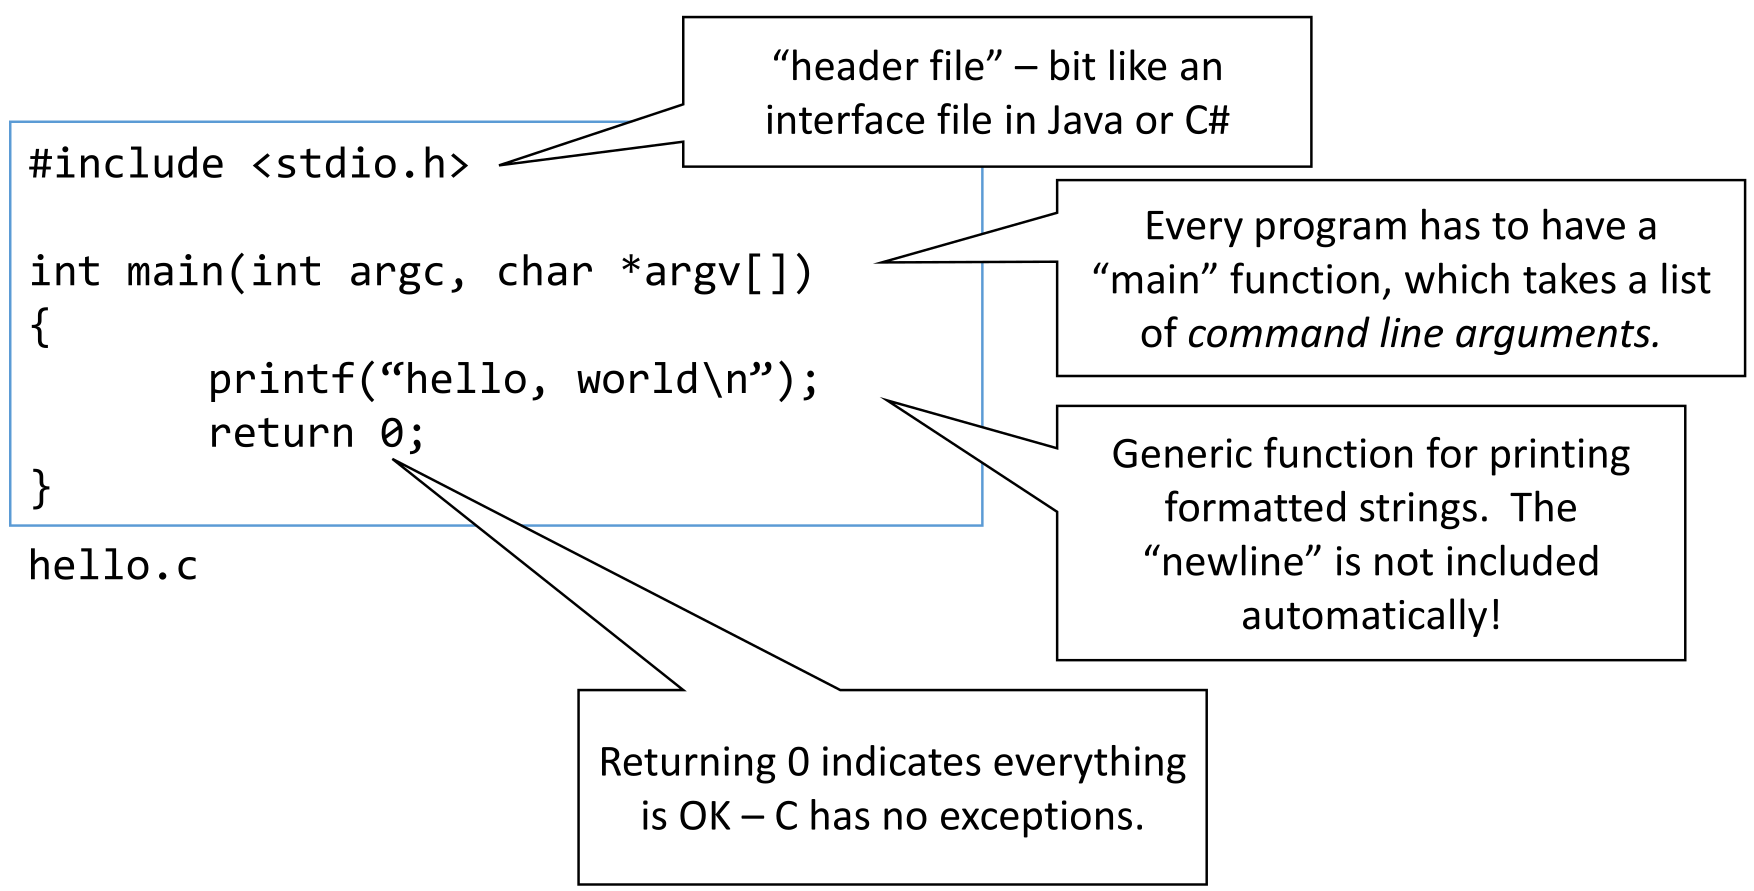
\includegraphics[width=0.8\textwidth]{02_exCode.png}

\subsubsection{Workflow}
Programmers write source code \code{.c} files and header files \code{.h}. At first, macros get substituted. Each of these files is compiled into assembly \code{.s} and then into object files \code{.o}. Object files are linked with their external libraries \code{.a} and we get an executable file. There are also libraries (shared libraries) \code{.so} which are dynamically linked while running the code.

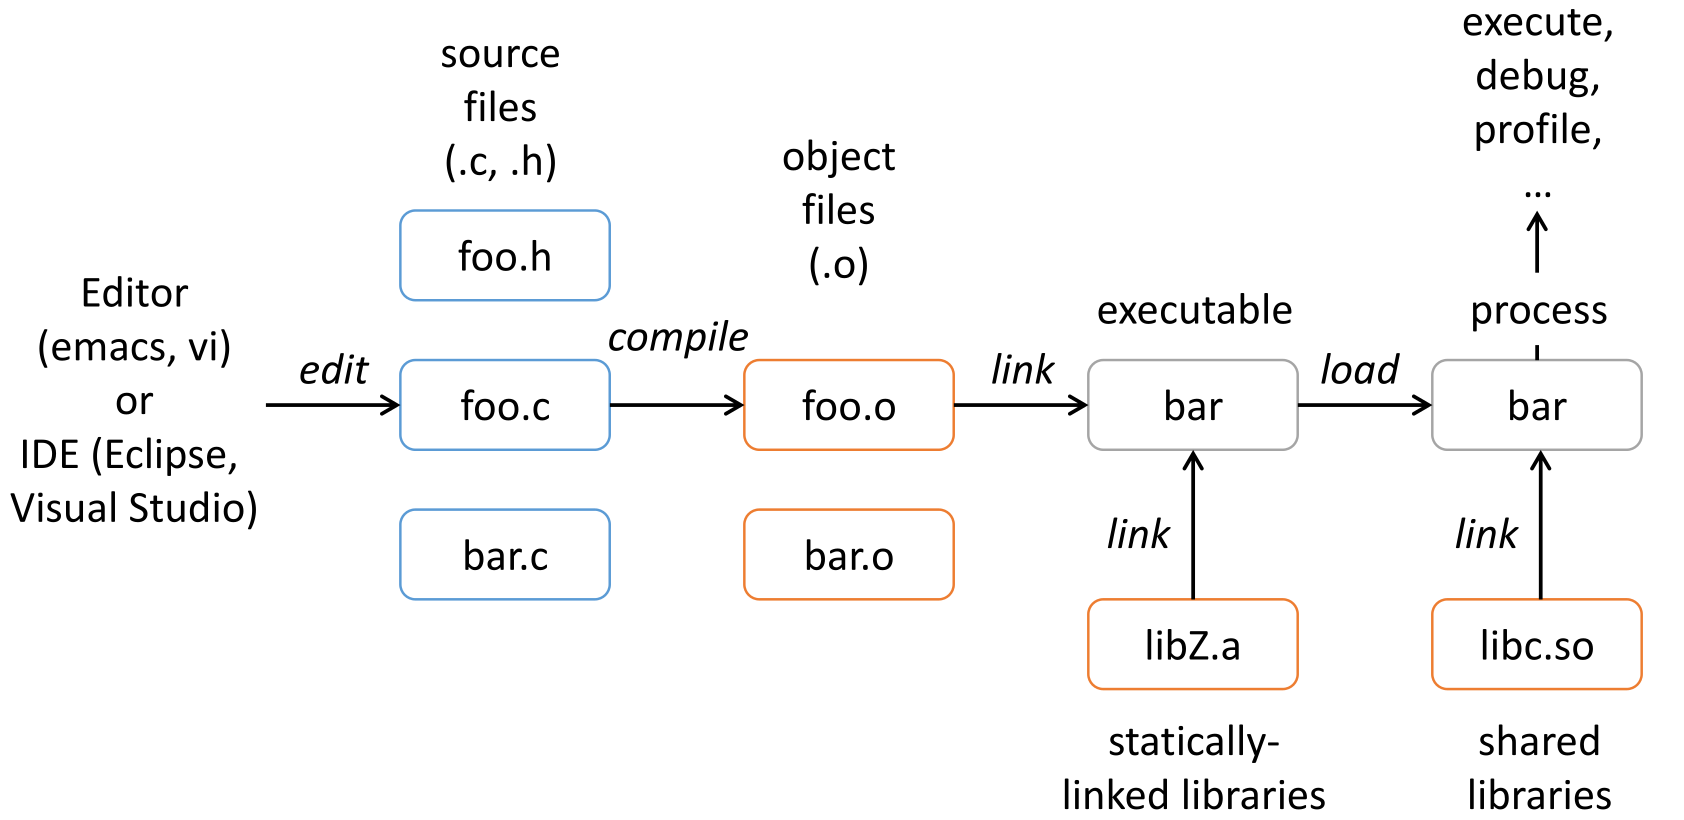
\includegraphics[width=0.8\textwidth]{02_workflow.png}

\code{gcc} is the \textit{compiler} (it does also all other parts of the workflow) we use in all exercises in this lecture.

We can stop the compilation at each stage:

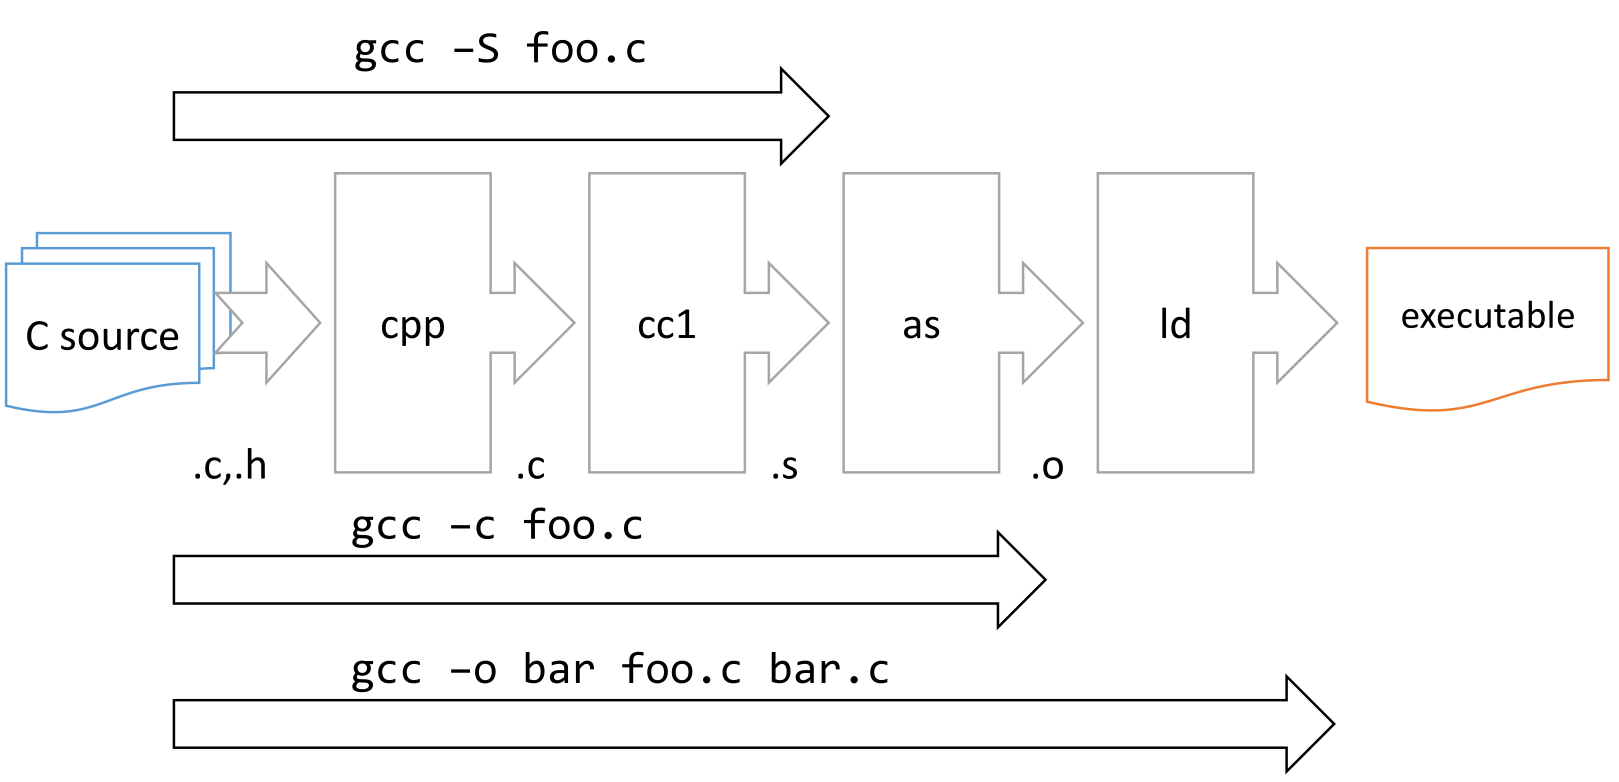
\includegraphics[width=0.8\textwidth]{02_gcc.png}

\subsection*{Control Flow}

\subsubsection{Conditionals}
They are written pretty much are we are used to.

\paragraph{If}
\begin{lstlisting}
if (Expression) {
    Statement_when_true
} else {
    Statement_when_false
}
\end{lstlisting}

The brackets can be omitted when the statements are just one line.
\begin{lstlisting}
if (Expression) Statement_when_true
else Statement_when_false
\end{lstlisting}

\paragraph{Switch}
If we not not break on a successful condition, multiple conditions may be executed.
\begin{lstlisting}
switch (Expression) {
        case Constant_1: Statement; break;
        case Constant_2: Statement; break;
        ...
        default: Statement; break;
}
\end{lstlisting}

\subsubsection{Loops}
The syntax of the three loop types available in C are as we are used to from other languages. 

If the statement is just one line, they may we written as:
\begin{itemize}
    \item \code{for (Initial; Test; Increment) Statement}
    \item \code{while (Expression) Statement}
    \item \code{do Statement while (Expression)}
\end{itemize}

\subsubsection{Other Statements}

\paragraph{Break}
Is used to break out of the current loop/switch. Unlike in Java, we cannot give a label.

\paragraph{Continue}
Stops current iteration of loop. Unlike in Java, we cannot give a label.

\paragraph{Goto}
\code{goto Label} jumps straight to \code{label}. It is controversial, but occasionally very useful. It makes code hard to read.

\subsubsection{Functions}
Functions are very similar to Java. They have a name, return type, argument types and a body.

\code{type name(paraType paraName) {body}}

The entry point to each C program is the \code{int main(int argc, char *argv[]) {body; return 0}} function. \code{argc} is the number of parameter and \code{*argv} a list of string parameter.

\code{return (Expression)} is used to return a value (may be computed by an expression) of a valid type (must conform to the defined return type).

\subsubsection{I/O}
\code{printf()} is used for outputs. The general format is that the first argument is the format string, containing special *replacement delimiters*, followed by the values to be inserted into the string. The number as well as the type of the variables must match the one in the format string.

\code{man 3 printf} for docs. 

\subsection*{Types}

\paragraph{Declarations}
Similarly as in Java, before a variable can be used, it must be declared \code{type name;}. Declaration and assignment can be combined into a single statement \code{type name = value;}.

\subparagraph{Scope}
Variables declared inside a block have a scope of only this block. Variables which are not defined inside a block have a scope of the entire program. 

\subparagraph{Static}
\code{static} in C is very different than in Java. Its meaning depends on its scope (/if it is inside/outside a block). If inside a block, the value of this variable persists between function calls. If static is used in a variable declared outside any block, the static makes that this variables is only accessible to this file (compilation unit) instead of the entire program.

\subsubsection{Types and Sizes}
\begin{table}[H]
    \centering
    \begin{tabular}{c c}
        C data type & Intel x86-64\\
        \hline
        char & 1\\
        short & 2\\
        int & 4\\
        long & 8\\
        float & 4\\
        double & 8\\
        long double & 10/16\\
    \end{tabular}
\end{table}

\subsubsection{Numbers}
Integers are signed by default. To make it more explicit, \code{signed} or \code{unsigned} can be prepended.

In standard, \code{int} have a size of $4$ bytes. Sometimes we want larger or smaller ints. In such cases we can use \code{<stdint.h>}, which provides extended integer types:
\begin{itemize}
    \item Signed: \code{int8\_t},\code{int16\_t}, \code{int32\_t}, \code{int64\_t}
    \item Unsigned: \code{uint8\_t}, \code{uint16\_t}, \code{uint32\_t}, \code{uint64\_t}
\end{itemize}

Conversion between different types is complicated and determined by the hardware. Between different integer types as well as between different floating types there is implizite conversation. Between anything else, we can use explizite conversation.

\subsubsection{Booleans}
Booleans are integers. Zero means false, anything else means true. Negation turns zero into non-zero and vice-versa. However, C99 supports \textit{real} boolean types via \code{<stdbool.h>}.

\subsubsection{Statements as Expressions}
Any C statement is also an expression. This means that any statements returns a integer ($\to$ boolean) value. This also counts for loops, assignments etc. which do not explicitly return any value.

For example assignment statements return the value they are assigned. We could use the following code to check for errors in a function call.
\begin{lstlisting}
int rc;
if (rc = myFunc()) {
    # error
} else {
    // everything good
}
\end{lstlisting}

\subsubsection{void}
\code{void} is a type which has no value. Pointers have typically a type assigned. \code{void} is used for untyped pointers (make them point to raw memory). We also use it for declaring functions without return value.

    %! TEX root=./main.tex

\lecture{Ex 1}{Week: 1}{}

\subsubsection{Bit Mask}
Bit masks can be used to:
\begin{description}
    \item[Delete] and \textbf{test} bits with AND
    \item[Set] bits with OR
    \item[Flip] bits with XOR
\end{description}

Test if $i$-th bit is $1$: \code{result = (input \& (1<<i))}

Flip if $i$-th bit is $1$: \code{result = (input \^ (1<<i))}

Set if $i$-th bit is $1$: \code{result = (input | (1<<i))}

    %! TEX root=./master.tex

\lecture{3}{Week: 2}{Continue Introduction to C and Integers}

\subsection*{Operators}
Operators and their precedence.

\includegraphics[width=\textwidth]{03_01_operators.png}

\subsubsection{Assignment}
Beside the ternary operator, assignment operators are the only operators which are right-to-left associative while all other operators are left-to-right associative.

As said before, assignments are expressions to (unlike in most other languages).

\subsubsection{Post-/Pre-Increment}
They work as we are used to from Java. We can also apply them to pointers. In that case the pointer value is not incremented by one but by the size of the type of the pointer.

\subsubsection{Casting}
Casting is a prefix operator \code{(newType) value;} which takes a value of a certain type and casts it to another designated type. The bit-representation does usually not change (but sometimes it does). E.g. when casing a small singend integer to a larger singed integer, the leading most significant bits is copied over into the extended region.

\subsection*{Arrays}
An array is a finite vector of values of the same type. They are arranged contiguously in memory. (Most) C compilers do not check array bounds. The indexed as usual, starting at $0$ up to $N-1$ (aka. C++ indexing :P ).

Even though arrays are defined with a certain length, given a array we cannot get its length.

\subsubsection{Basics}
\paragraph{Definition}
The are defined using \code{type name[length];}. E.g. a float array with $5$ elements is defined with \code{float data[5];}.

After the definition, no values are assigned to the array, meaning we do not know what elements the array holds. So we cannot assume that it is all zero or something. In order to initialize each value to zero, we can use \code{type name[length] = \{\};}.

We can also initialize by assigning a set of values like \code{type name[length] = \{val1, val2, ... \}}.

\paragraph{Assignment}
Assignment is done one-by-one using \code{var[i] = val}.

\paragraph{Access}
Arrays are accessed using \code{var[i]}.

\subsubsection{Multidimensional Arrays}
Multidimensional arrays are stored in row-major in a continuous array. Meaning they are stored as $a[0][0], \dots, a[1][0], \dots, a[2][0], \dots, a[2][2]$.

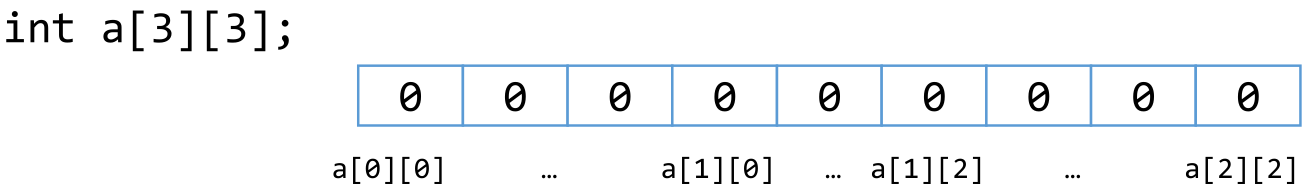
\includegraphics[width=0.8\textwidth]{03_multiDimArray.png}

When viewed as a matrix, the first brackets defines the number of columns and the second bracket the number of rows.

\subsubsection{Strings}
There is no string type in C. Instead strings are an array of chars. The end of the array is marked by the null character $\\0$. We could assign it directly as an array of chars \code{char arr[3] = \{'a', 'b', '\\0'\}}. This way we must add the null character explicitly. It is often easier to assign the sting directly as \code{char arr[3]= "ab"}.

Very important is that when setting the length of the array, we keep in mind that the null character requires some space too.

Given that strings have a special termination character, unlike for general arrays, for char arrays we can determine the length of the array given the array.

\paragraph{String Manipulation}
There are no built-in methods for manipulating strings, but there are many libraries which support this. For example \code{<string.h>} is such a library and their manipulation methods have the format \code{strxxx()}.

\code{strcpy} copies a given string, \code{strcat} concatenates two given strings, \code{strcmp} compares two strings of equality etc.

\subsection*{Integers}

\subsubsection{Represent Integers}
Integers are stored as a sequence of bytes. x86 uses little-endian, meaning that the least significant byte comes first.

\subsubsection{Operations}
\paragraph{Bit-Level}
Manipulate single bits of any \textit{integral} data type (long, int, short, char, unsigned). The arguments can be viewed as bit vectors.

\begin{tabular}{c | c}
    $\&$ & and\\
    $|$ & or\\
    $\tilde{}$ & not\\
    $\hat{}$ & xor
\end{tabular}

We can also use the to represent and manipulate sets. We encode bit vectors in a certain way.

\paragraph{Logical}
Viewing data as true and false where $0$ means false and everything else true. Either of the two states is always returned. They apply to the vector as a whole.

\begin{tabular}{c | c}
    $\&\&$ & and\\
    $||$ & or\\
    $!$ & not
\end{tabular}

\paragraph{Shift}
\begin{itemize}
    \item Left shift: $x << y$ shifts bit-vector $x$ left by $y$ positions
        \begin{itemize}
            \item Fill right with $0$s.
        \end{itemize}
    \item Right shift: $x >> y$ shift bit-vector $x$ right $y$ positions
        \begin{itemize}
            \item Logical shift: fill with $0$s (always applied if int is signed)
            \item Arithmetic shift: replicate most significant bit (always applied if int is unsigned)
        \end{itemize}
\end{itemize}

The behaviour of negative numbers and numbers larger then the vectors is undefined.

\paragraph{Encoding}

Unsigned integers are encoded in such a way, that with increasing position (LSB to MSB), the factor of two increases: $\sum_{i=0}^{w-1} x_i \cdot 2^i$.

With two's complements encoding we have to consider that the MSB is the sign bit. If is set, $2^{w-1}$ is subtracted of the number represented by the last $w-2$ bits: $-w_{w - 1} \cdot 2^{w - 1} + \sum_{i=0}^{w - 2} x_i \cdot 2^i$.

\paragraph{Ranges}
\begin{itemize}
    \item UMin $= 0$
    \item UMax $= 2^w -1$
    \item TMin $=-2^{w - 1}$
    \item TMax $=2^{w-1} - 1$
\end{itemize}

Depending on the word size of the number, we can represent different ranges:

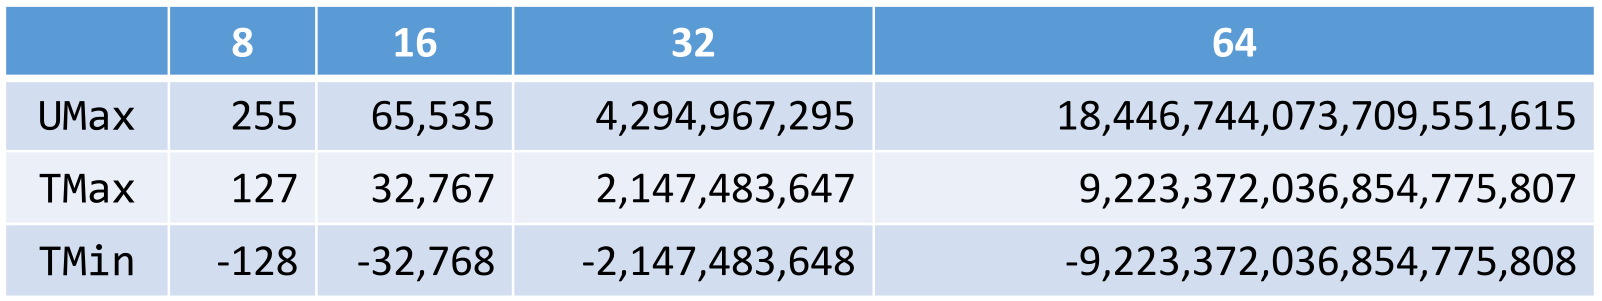
\includegraphics[width=0.8\textwidth]{03_wordSizeRange.png}

From this table we can notice two interesting things:
\begin{enumerate}
    \item $|\text{TMIN}| = |\text{TMAX} + 1$. I.e. we can represent one negative number more than positive (asymmetric range)
    \item UMAX $= 2 \cdot \text{TMAX} + 1$
\end{enumerate}

In practice, we can use \code{<limits.h>} which provides \code{ULONG\_MAX}, \code{LONG\_MAX}, \code{LONG\_MIN}... to get these bounds.

\paragraph{Visualisation}
When comparing the interpreted signed/unsigned number of a certain bit patters, we see that for the lower halve of numbers, the signed and unsigned numbers are equivalent. Fur the other halve of numbers, i.e. all which have MSB of $1$, we have to add $2^{\text{word size}}$ to get from signed to unsigned. 

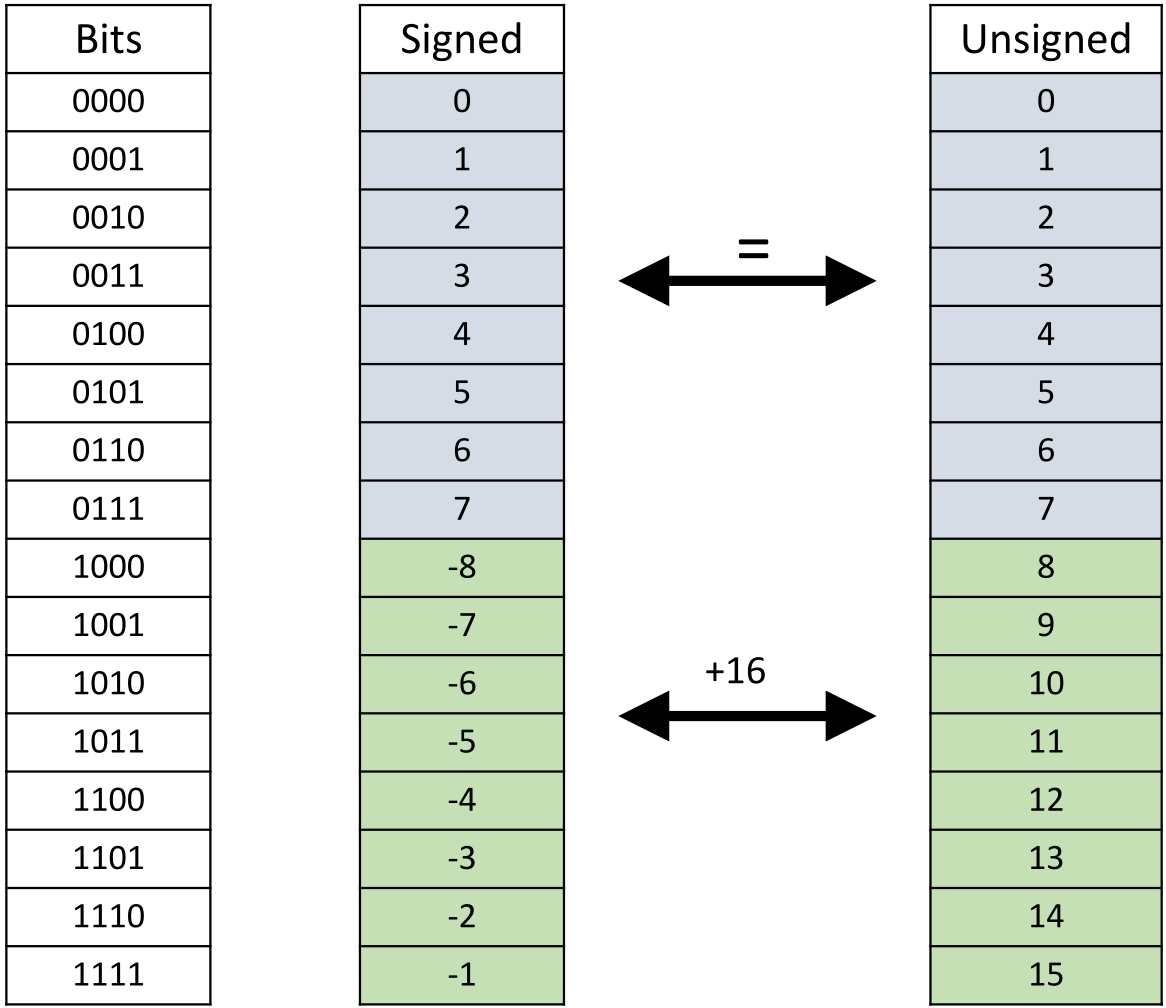
\includegraphics[width=0.8\textwidth]{03_signedUnsignedMap.png}

The difference between signed and unsigned can also be seen as a shift of the ranges.

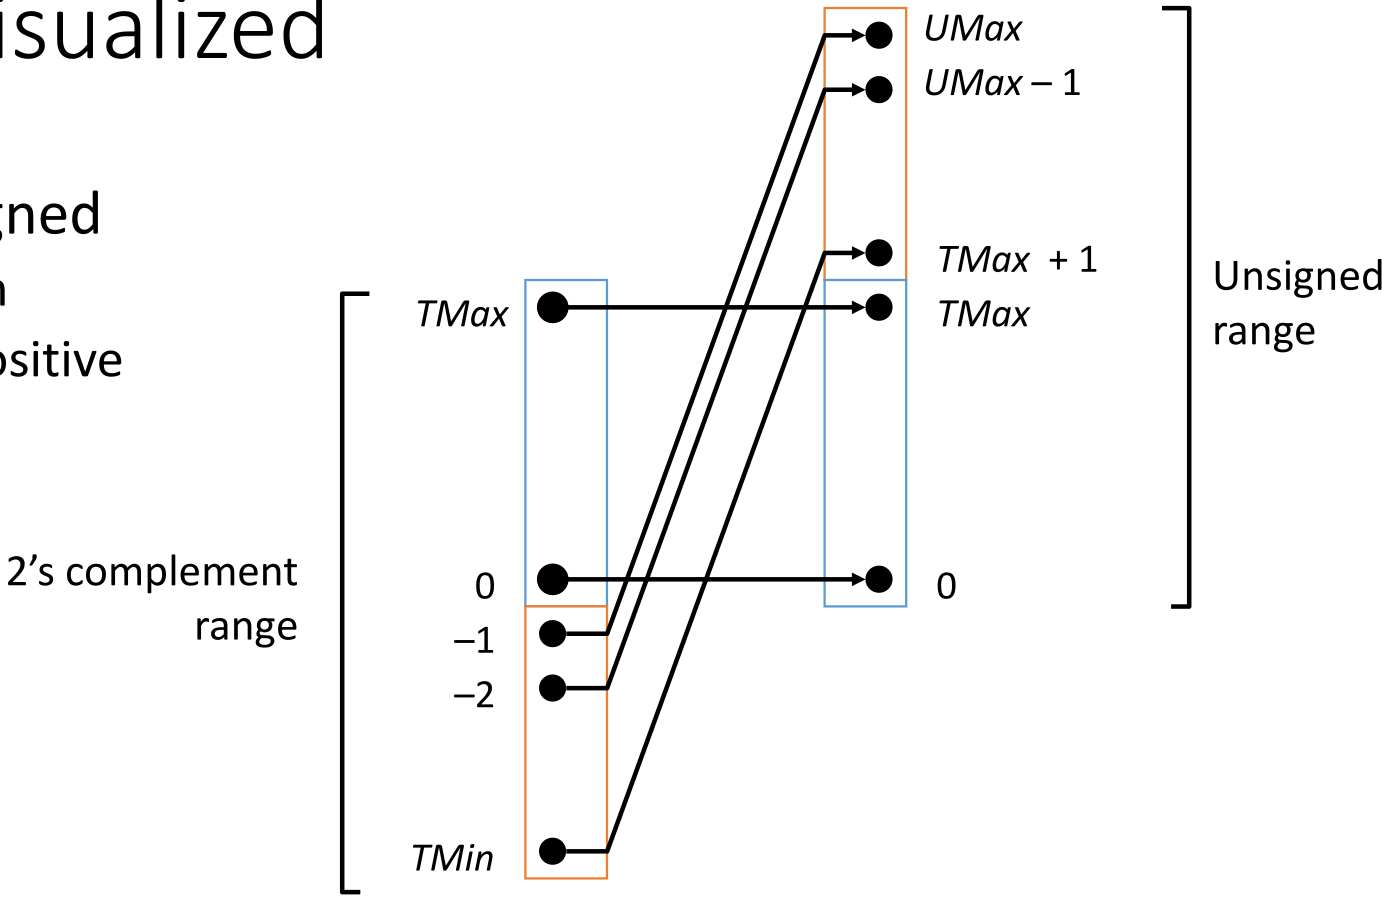
\includegraphics[width=0.8\textwidth]{03_signedUnsignedRange.png}

\paragraph{Signed vs Unsigned}
By default numbers are considered as signed. In order to get a unsigned number, we have to suffix the number with a \code{U}.

In order to get from one to the other, we have to cast the number. There are two different ways to cast a number:

\subparagraph{Explicit}
Given signed number \code{int a;} we can cast it to unsigned number \code{unsigned b} using \code{b = (unsigned) a;}. The other ways around, casting from unsigned \code{unsigned b} to signed number \code{int a} is done using \code{a = (int) b;}.

\subparagraph{Implicit}
This kind of conversion happens when we assign a signed/unsigned number to a unsigned/signed. I.e. given \code{int a; unsigned b;} and we assign \code{a = b;} or \code{b = a;}.

Beside assignments, implicit conversion also happens when we mix signed and unsigned numbers in an expression. It that case the signed number is casted implicitly to a unsigned. 

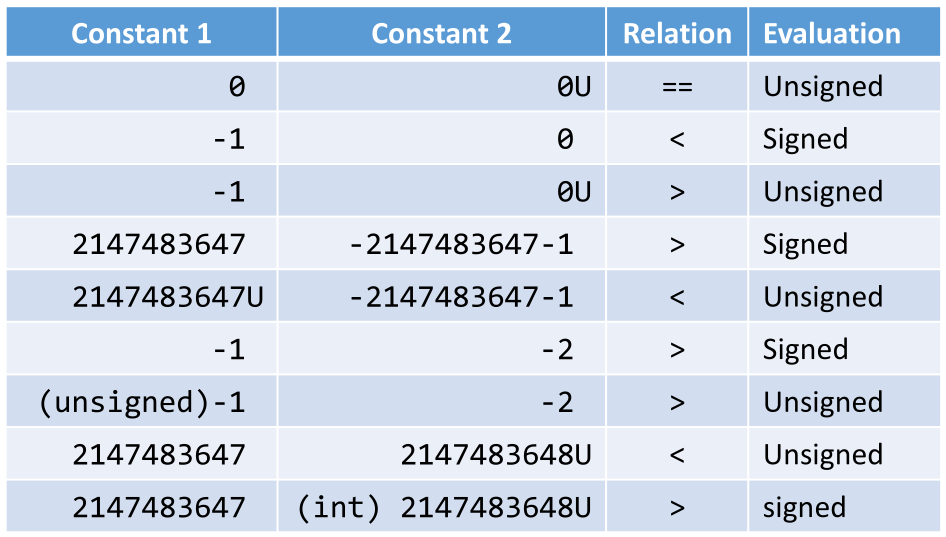
\includegraphics[width=0.8\textwidth]{03_02_numbercasting.png}

If not done by purpose, this can have undesired side effects including security concerns.

    %! TEX root = ./master.tex

\lecture{4}{Week: 2}{Continue Integers}

\subsubsection{Sign extension}
Given a $w$ bit signed integer $x$, convert it to a $w + k$ bit signed integer with the same value.

We do that by coping the most significant bit of $x$ and copy it to all $k$ new bits

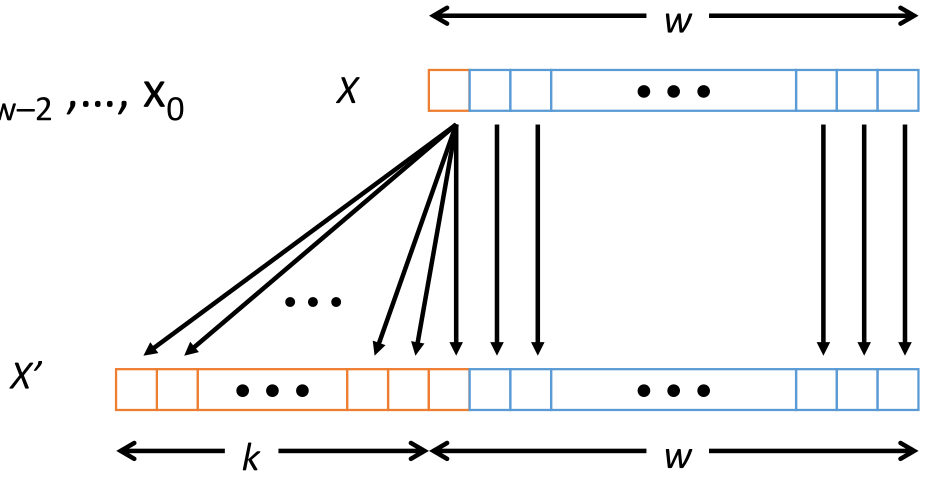
\includegraphics[width=0.8\textwidth]{04_signExtend.png}

For unsigned numbers, the number is padded with zeros at the beginning.

C does this sign extend automatically for us.

\subsubsection{Truncation}
Throws away the left bits. For unsigned numbers it represents the modulo operator. For signed integers it is also like modulo, but it does it in a special way (negative number may get positive and vice versa).

Also, only small numbers remain unchanged.

\subsubsection{Addition and Subtraction in C}
\paragraph{Negation}
Number $x$ can be negated using $\tilde x + 1 == -x$.

It follows that $\tilde x + x == 111 \dots 111 == -1$

\paragraph{Unsigned addition}
When adding two unsigned number $u$ and $v$ of length $w$, we get a number of length $w + 1$.

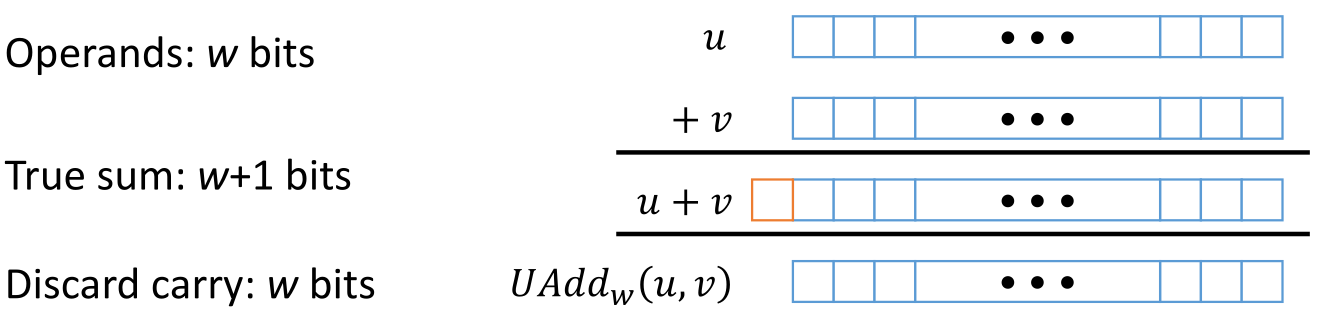
\includegraphics[width=0.8\textwidth]{04_unsignedAdditionEquation.png}

The function $UAdd_w(u,v)$ ignores the extra bit which would be required if the sum overflows the $w$ bits. This function can also be seen as:

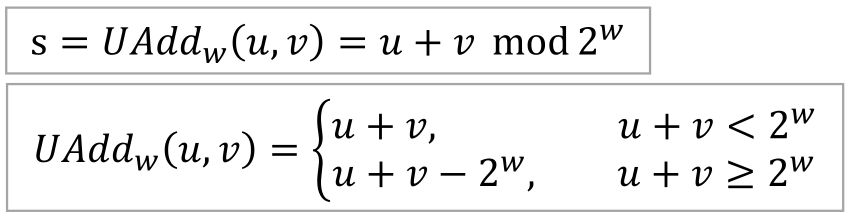
\includegraphics[width=0.8\textwidth]{04_unsignedAdditionFormula.png}

Then the sum overflows, it wraps around.

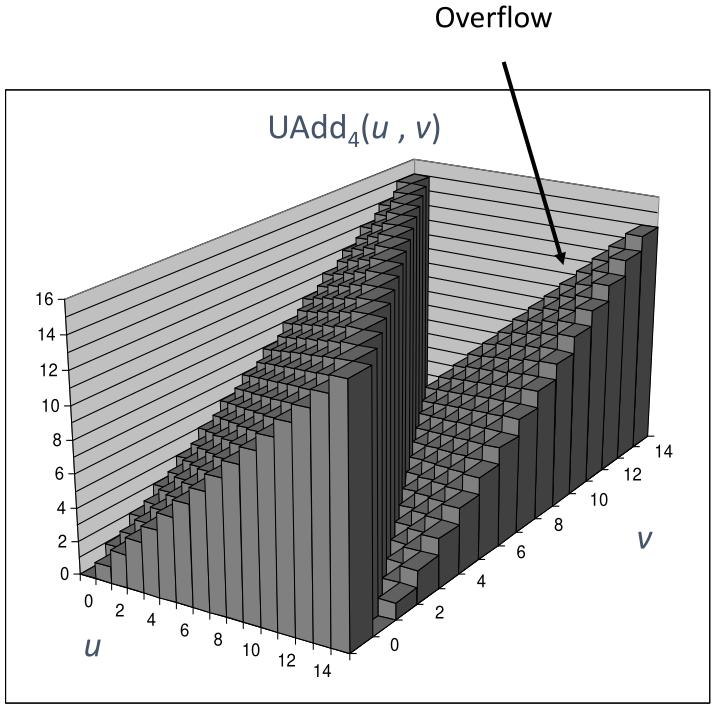
\includegraphics[width=0.8\textwidth]{04_01_unsignedAddition.png}

The $Uadd_w$ function is the classical unsigned addition operator in C. There are certain compilers which provide some possibility to retrieve a possible overflow.

$UAdd_w(u,v)$ is an Abelian group (Closed, Commutative, Associative, Identity, Inverse)

\paragraph{Two's complement addition}
When adding two signed number $u$ and $v$ of length $w$, we get a number of length $w + 1$.

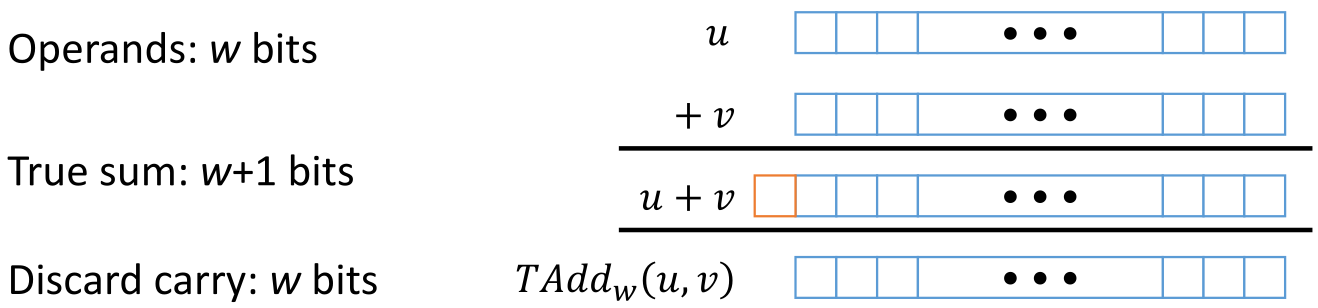
\includegraphics[width=0.8\textwidth]{04_signedAdditionEquation.png}

The function $TAdd_w(u,v)$ ignores the extra bit which would be required if the sum overflows the $w$ bits.

$TAdd_w(u,v)$ behaves identical to $UAdd$ in the bit level interpretation. But the overflow behaves differently (are interpreted differently). Positive overflow gives a negative number, a negative overflow gives a positive number.

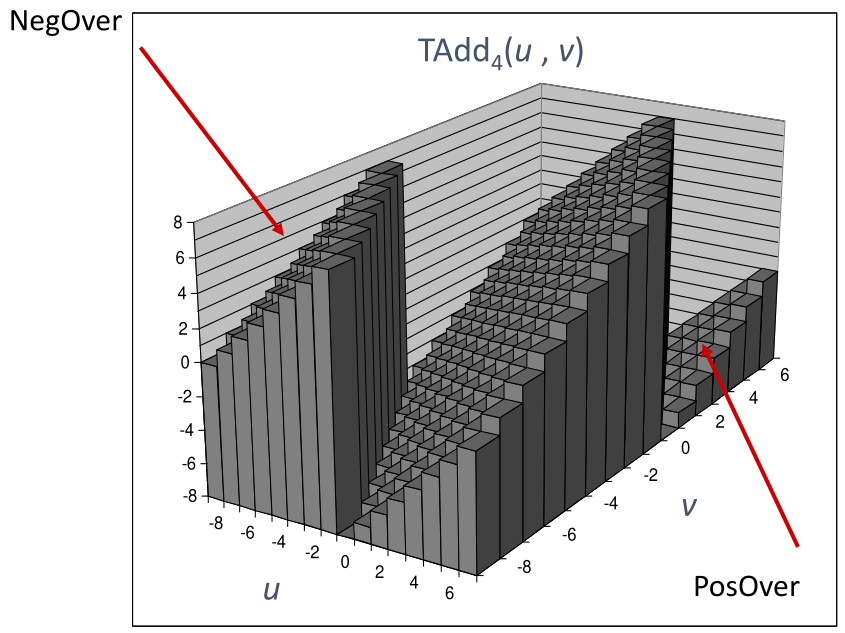
\includegraphics[width=0.8\textwidth]{04_02_signedAddition.png}

The function can be seen as:

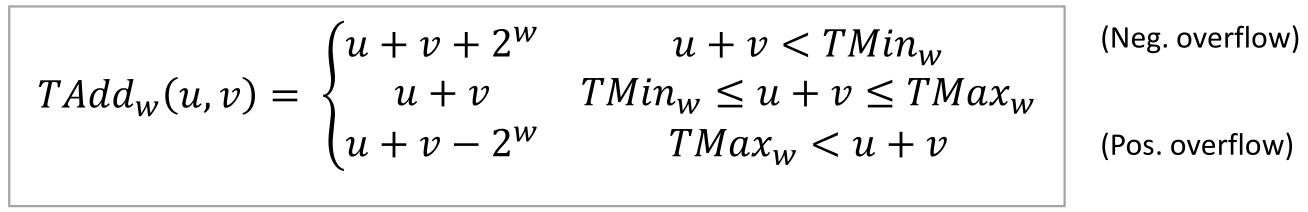
\includegraphics[width=0.8\textwidth]{04_signedAdditionFormula.png}

$TAdd$ is isomorphic to $UAdd$ and $TAdd$ forms a group (closed, commutative, associative, identity, inverse).

\subsubsection{Integer multiplication in C}

\paragraph{Unsigned Multiplication}
When multiplying two unsigned number $u$ and $v$ of length $w$, we get a number of length $2w$.

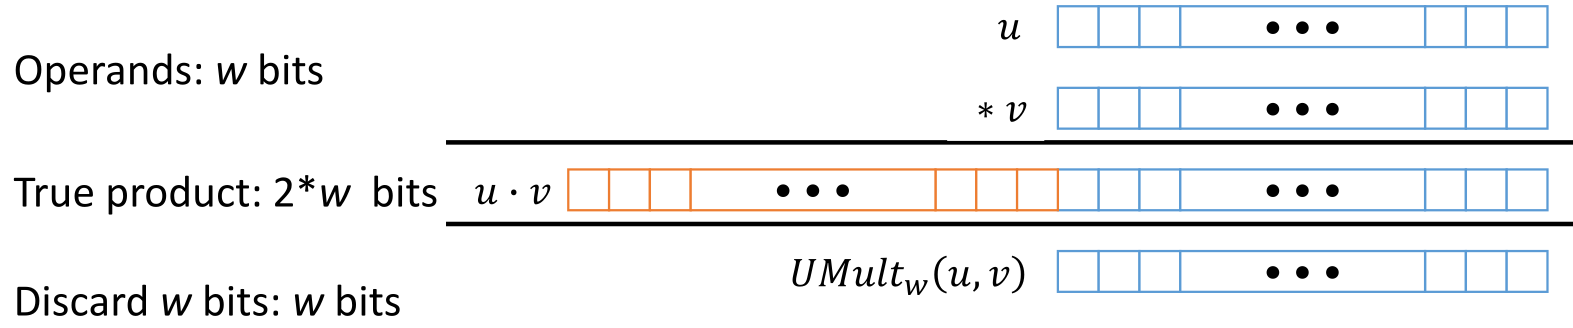
\includegraphics[width=0.8\textwidth]{04_unsignedMultiplyEquation.png}

The operator $UMult_w(u,v)$ truncates the overflowing bits. The formula can be seen as:

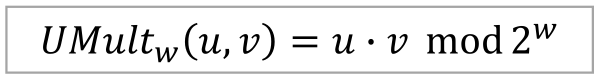
\includegraphics[width=0.8\textwidth]{04_unsignedMultiplyFormula.png}

In order that the product is exact $x$ and $y$ must satisfy $0 \le x \cdot y \le (2^w -1)^2$

$UMULt_w$ forms a commutative ring with $UAdd$.

\paragraph{Signed Multiplication}
When multiplying two signed number $u$ and $v$ of length $w$, we get a number of length $2w$.

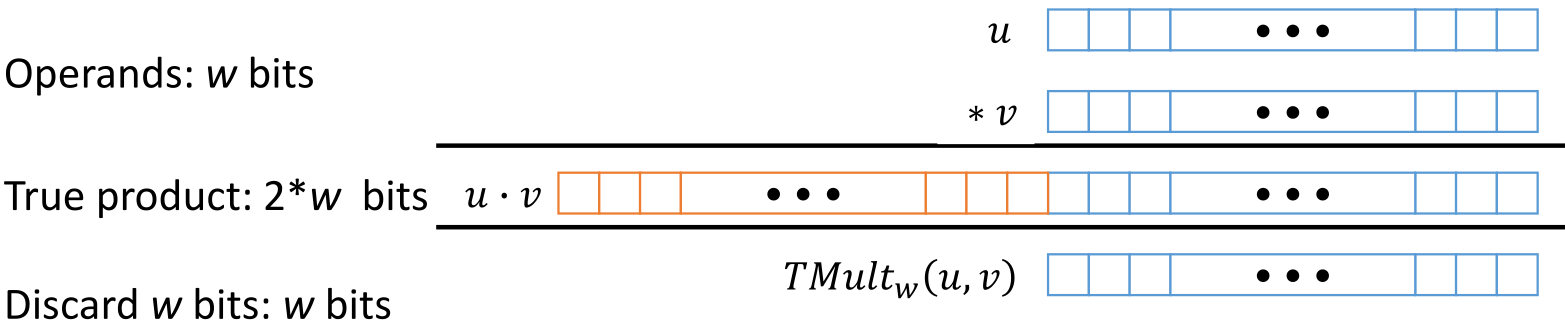
\includegraphics[width=0.8\textwidth]{04_signedMultiplicationEquation.png}

The operator $TMult_w(u,v)$ ignores the overflowing bits. Some hardware puts overflowing bits into a special register, but they are normally not accessibly in C.

The minimal product which can be represented accurately is $x \cdot y \ge (-2^{w - 1}) \cdot (2^{w - 1} - 1)$. And the greatest number is $x \cdot y \le (-2^{w -1})^2$.

\subsubsection{Multiplication and Division Using Shifts}
\paragraph{Multiplication}
As we have seen, the shift operator shifts the binary representation of a number. Regarding the interpreted number, $u << k$ results in $u \cdot 2^k$. This is valid for signed and unsigned numbers.

When shifting a signed/unsigned number of length $w$ by $k$, the $k$ over flowing bits are truncated.

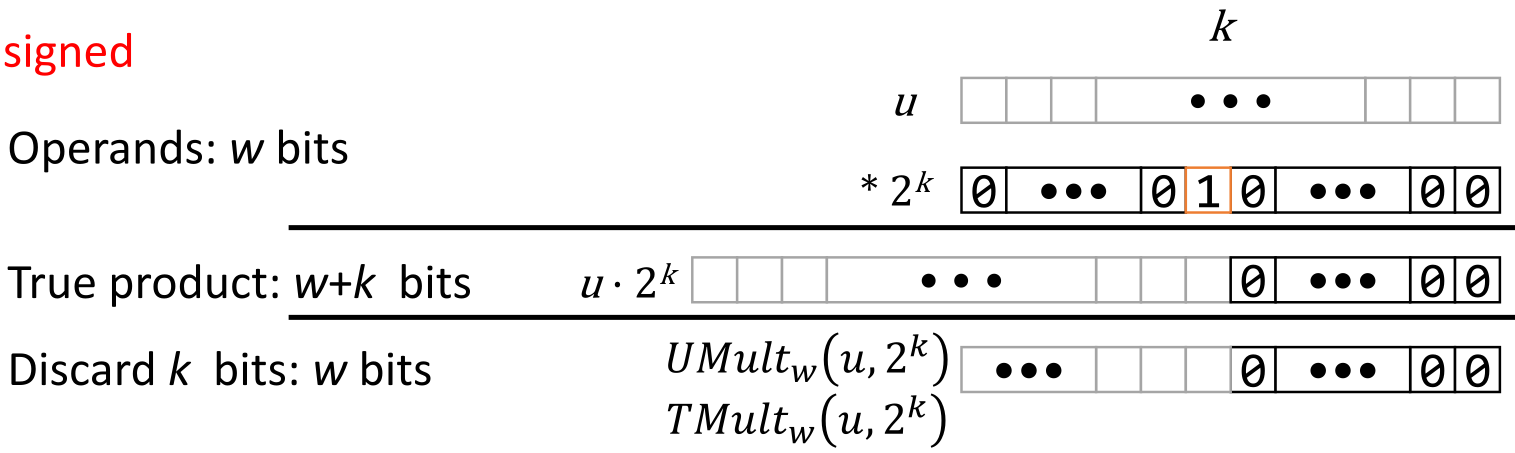
\includegraphics[width=0.8\textwidth]{04_powerOfTwo.png}

Multiplication is much more complex than simple shifts. Therefore, to calculate $u \cdot 24$ we may write $(u << 5) - (u << 3)$. But modern compiler do such thinks (and even better optimisations) for us, therefore we should not do it.

\paragraph{Division}
Equally as with multiplication, shifts can be used for division of power of twos. $u >> k$ gives $\lfloor \frac{u}{2^k} \rfloor$. The underflowing $k$ bits get truncated.

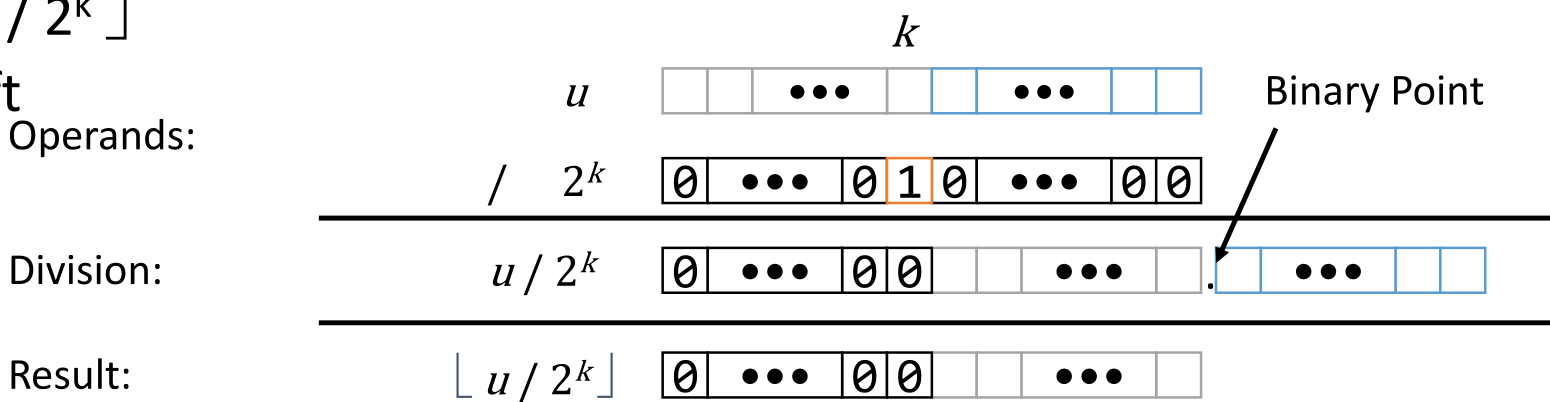
\includegraphics[width=0.8\textwidth]{04_powerOfTwoDivide.png}

Even though this works for unsigned and signed number, for signed numbers the results may be wrong for negative numbers. 
This is because we round down, but actually we would like to round towards $0$. We can fix that by computing $\lfloor \frac{(s + 2^k - 1)}{2^k} \rfloor$. In C this is equivalent to $(s + (1 << k) -1) >> k$. This formula works for positive and negative numbers.

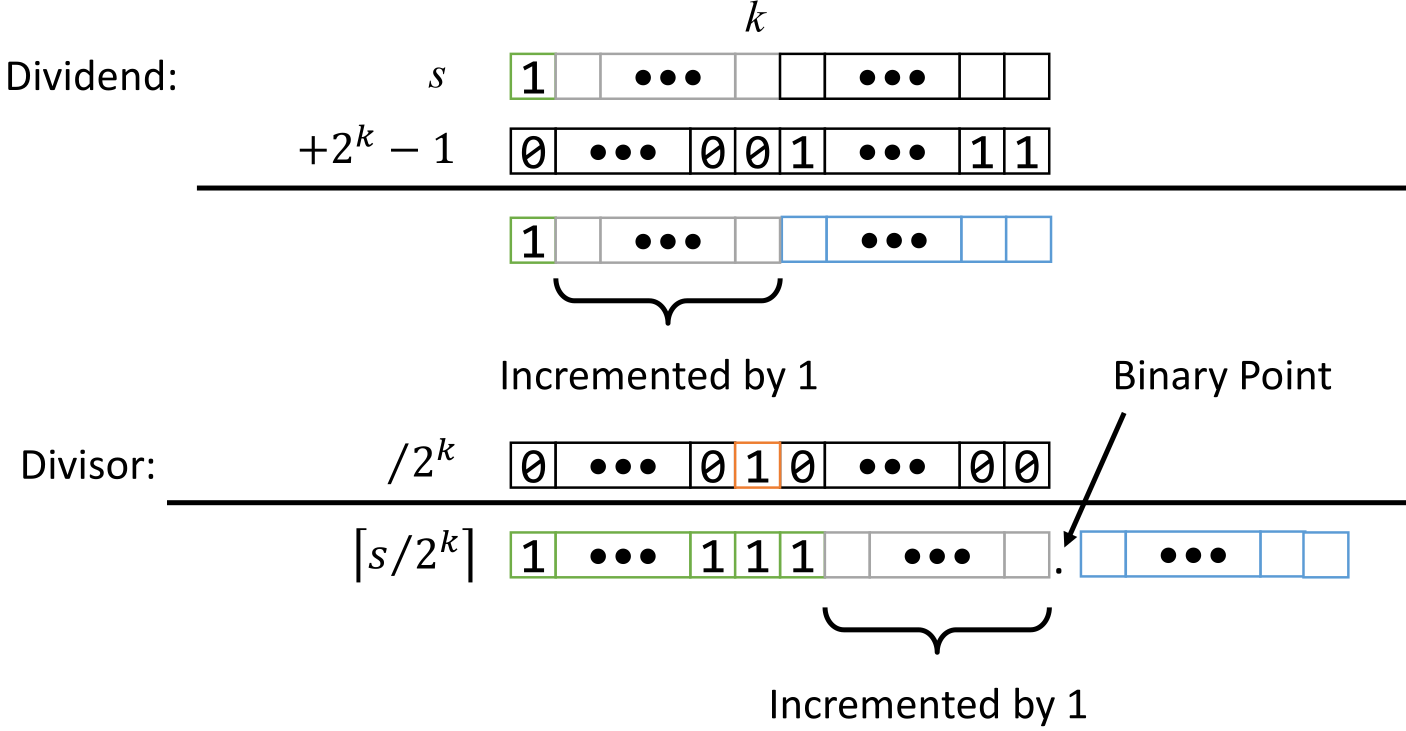
\includegraphics[width=0.8\textwidth]{04_powerOfTwoDivideCorrect.png}


Again, the compiler can translate divisions into shifts. For unsigned numbers, it applies the first formula, for signed numbers the second one.

\subsubsection{C Integer puzzles}
In the following are some integer related puzzles to solve.

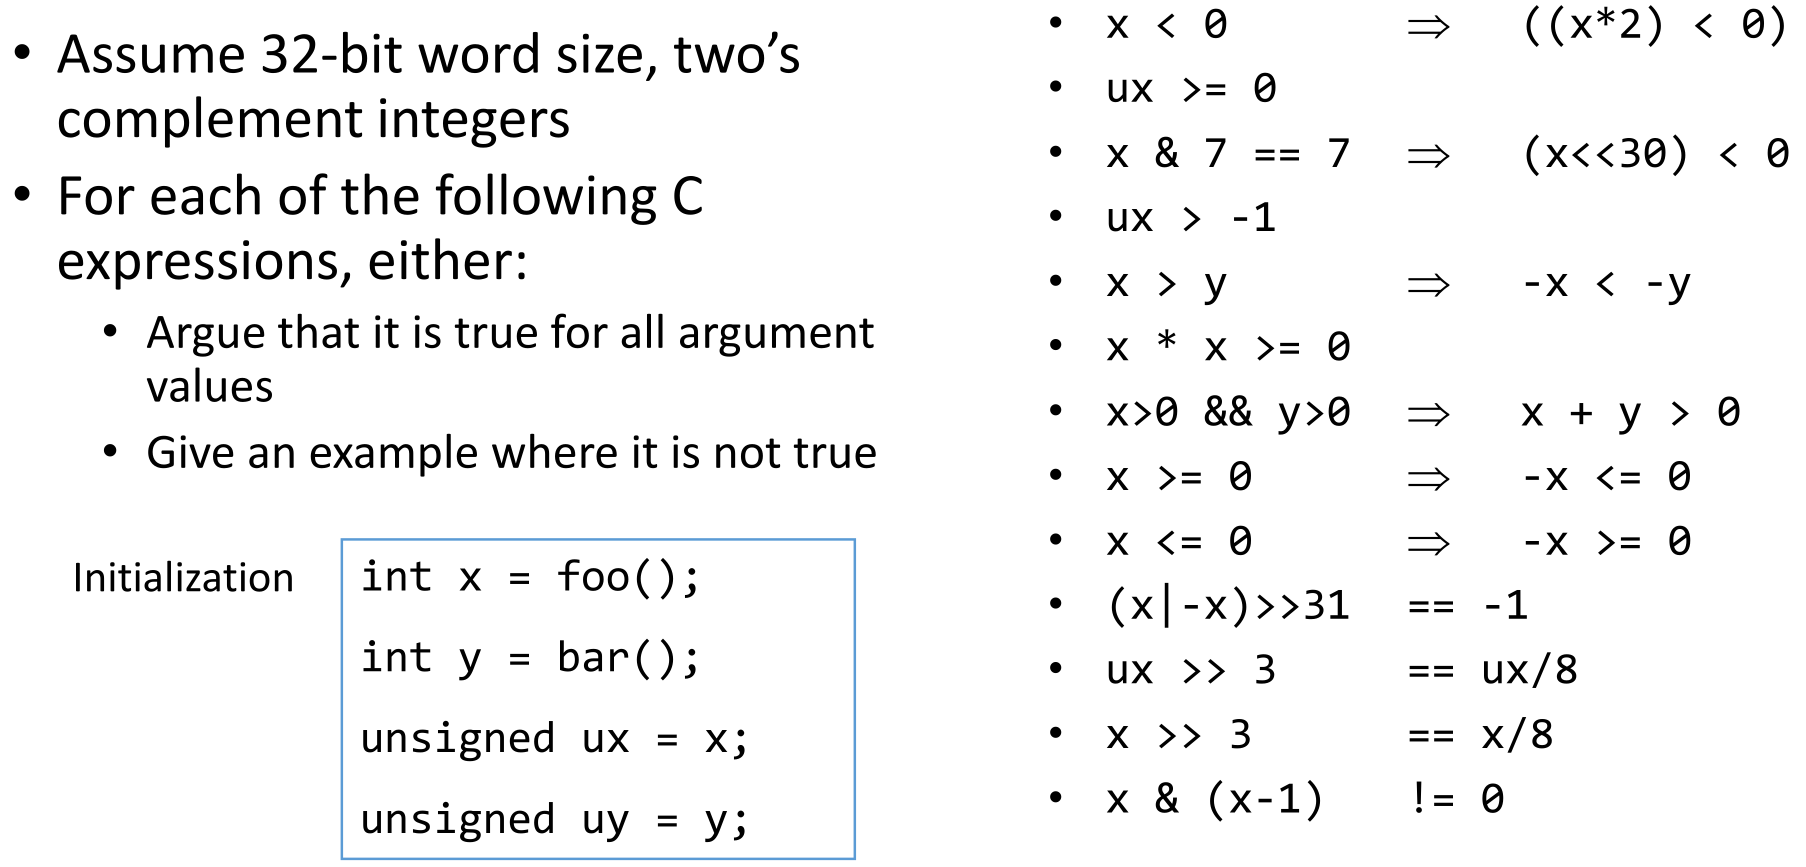
\includegraphics[width=0.8\textwidth]{04_integerPuzzle.png}

    %! TEX root=./main.tex

\lecture{Ex 2}{Week: 2}{}

\subsubsection{Header Files and Modules}

\paragraph{Definition vs. Declaration}
There is a difference between declaration and definition:
\begin{itemize}
    \item Declaration gives the signature of the function / variable.
    \item Definition gives the code /storage space for variables.
\end{itemize}

\paragraph{Header Files}
In order to share a function among different source file, we have to place the function declaration into the header file.

Using \code{\#include "mymodule.h"} the function can be included into other source files. Note the difference between the prior include and e.g. \code{\#include <stdio.h>}. The first one looks for header files in the same directory while the second one looks for system header files.

Header files are considered globally accessible. So one should only put there what is actually necessary like e.g. public interfaces.

Header files are actually copy-pasted into the source file during compilation. To prevent multiple imports (e.g. for nested modules), a guard structure should be used.

\paragraph{Compilation}
To compile programs which consists of multiple source files with their associated header files, we have to list all required source (not header) files for gcc.

\subsubsection{Makefile}
Makefiles are used to automate compilation. It it like defining functions for or complex compile commands. The general structure is

\begin{verbatim}
targets: prerequisites
    command
    command
\end{verbatim}

where \verb+target+ is the name of the function, in \verb+prerequisits+ we list all required source and header files and beneath we place the command(s) required for compilation.

We can also define rules for different tasks than only compiling like for build cleanup.

\subsubsection{gcc Flags}
Useful flags:

\begin{description}
    \item[Werror:] Make all warnings into errors.
    \item[Wpedantic:] Issue all the warnings demanded by strict ISO C and reject all programs that use forbidden extensions.
    \item[Wall:] Enable different warnings about questionable code.
    \item[fsanitize=address:] Instrument code to detect heap management errors.
    \item[fsanitize=undefined:] Instrument code to detect undefined behaviour at runtime.
    \item[fsanitize-address-use-after-scope:] Instrument code to detect addresses used when already out of scope.
    \item[fstack-protector-all:] Instrument code to detect buffer overflow on the stack.
\end{description}

In practice we should use something like:

\verb+gcc <FILES> -Wall -Wpedantic -Wextra -Werror -std=c99 -Wmissing-prototypes+

    %! TEX root = ./main.tex

\lecture{5}{Week: 3}{C Pointers}

\subsubsection{Address Space}
The OS gives each process an address space, which contains the virtual memory. The virtual memory is visible only to the process. Each byte is addressable and there are $2^{64}$ bytes of memory on a $64$ bit machine. The OS maps the virtual memory to the physical memory.
When the OS loads a program, the following steps are executed:

\paragraph{Loading a program}
\begin{itemize}
    \item create an address space
    \item inspect the executable file
    \item copy regions of the file into memory space
    \item do final linking, reallocation or other preparations
\end{itemize}

\subsubsection{Stack}
The stack is allocated in frames. The current procedure's frame always lies on the top of the stack. The frame stores local variables, return types etc. On recursive calls, for each recursion a new frame is pushed to the stack

\subsubsection{C Pointers}
Pointers are variables which store memory addresses. \code{\&x} gives the virtual address where the value of variable \code{x} is stored. With \code{\%p} its value can be printed. Pointers are declared using the format \code{type *name;}. Dereferencing a pointer means accessing the memory referred by the pointer. This way we can access the value at the address or write some value to the address. Double pointers are pointers which point to a pointer. They are declared using \code{type **name;}. Double pointers are mostly used for multidimensional arrays.

The address space layout randomization is responsible that the stack bases and shared library location addresses change for each execution. This is a security feature which makes debugging tougher. But it could be disabled.

\code{NULL} is a \textit{guaranteed-to-be-invalid} memory location and has type \code{void *}. Dereferencing \code{NULL} causes a segmentation fault. \code{NULL} is useful to mark end points and invalid addresses.

A \code{*} is used to indicate that a function returns a pointer as \code{int *getPtr()}.

\subsubsection{Pointer Arithmetic}
When incrementing a pointer by $1$, the value of the pointer (address) is incremented by the size of the type of the pointer. For integer this is e.g. $4$ bytes, for double $8$ bytes, for char $1$ byte etc... These values depend on the machine and compiler. The size can be evaluated using \code{sizeof(type)} or \code{sizeof(value)}.

\subsubsection{Arrays and Pointers}
An array is a collection of homogeneous data elements stored at contiguous memory adresses. A Pointer is a variable that stores a memory address. So pointers and arrays are different, but related things. The array name is an expression and treated as a pointer to the first element of the array \code{a == \&(a[0])}. We can access the array by the \textit{pointer} $+$ some offset. The compiler rewrites \code{A[i]} to \code{*(A+i)}, hence we could theoretically access arrays like \code{i[A]}.\\
However, the array name is different from the pointer when:
\begin{enumerate}
    \item The array is an operand of \code{sizeof()}
\begin{lstlisting}
int a[10]:
assert(sizeof(a) == 10 * sizeof(int));
assert(sizeof(&a[0] == sizeof(int *));
\end{lstlisting}
    \item The array's address is taken with \code{\&}
\begin{lstlisting}
int a[10];
assert(&a == a);
\end{lstlisting}
    \item The array is string literal initializer
\begin{lstlisting}
char a[] = "Hello!";
char *b = "Hello!"; // undef. behaviour when modified
\end{lstlisting}
\end{enumerate}
In C, parameters are passed as value (since there is nothing like a reference), with the only exception of arrays and functions. They are passed by pointers. Therefore, the following three formal arguments \code{int *arr}, \code{int arr[]} and \code{int arr[10]} are equivalent.\\ 
Arrays cannot be renamed, but we change the pointer.

\subsubsection{Passed by Reference}
Since C is passed by value, we can pass a reference by passing a pointer. However, this pointer is again passed by value and therefore can be modified in the scope of the functions.

\subsubsection{Examples}
Here some pointer declaration examples:

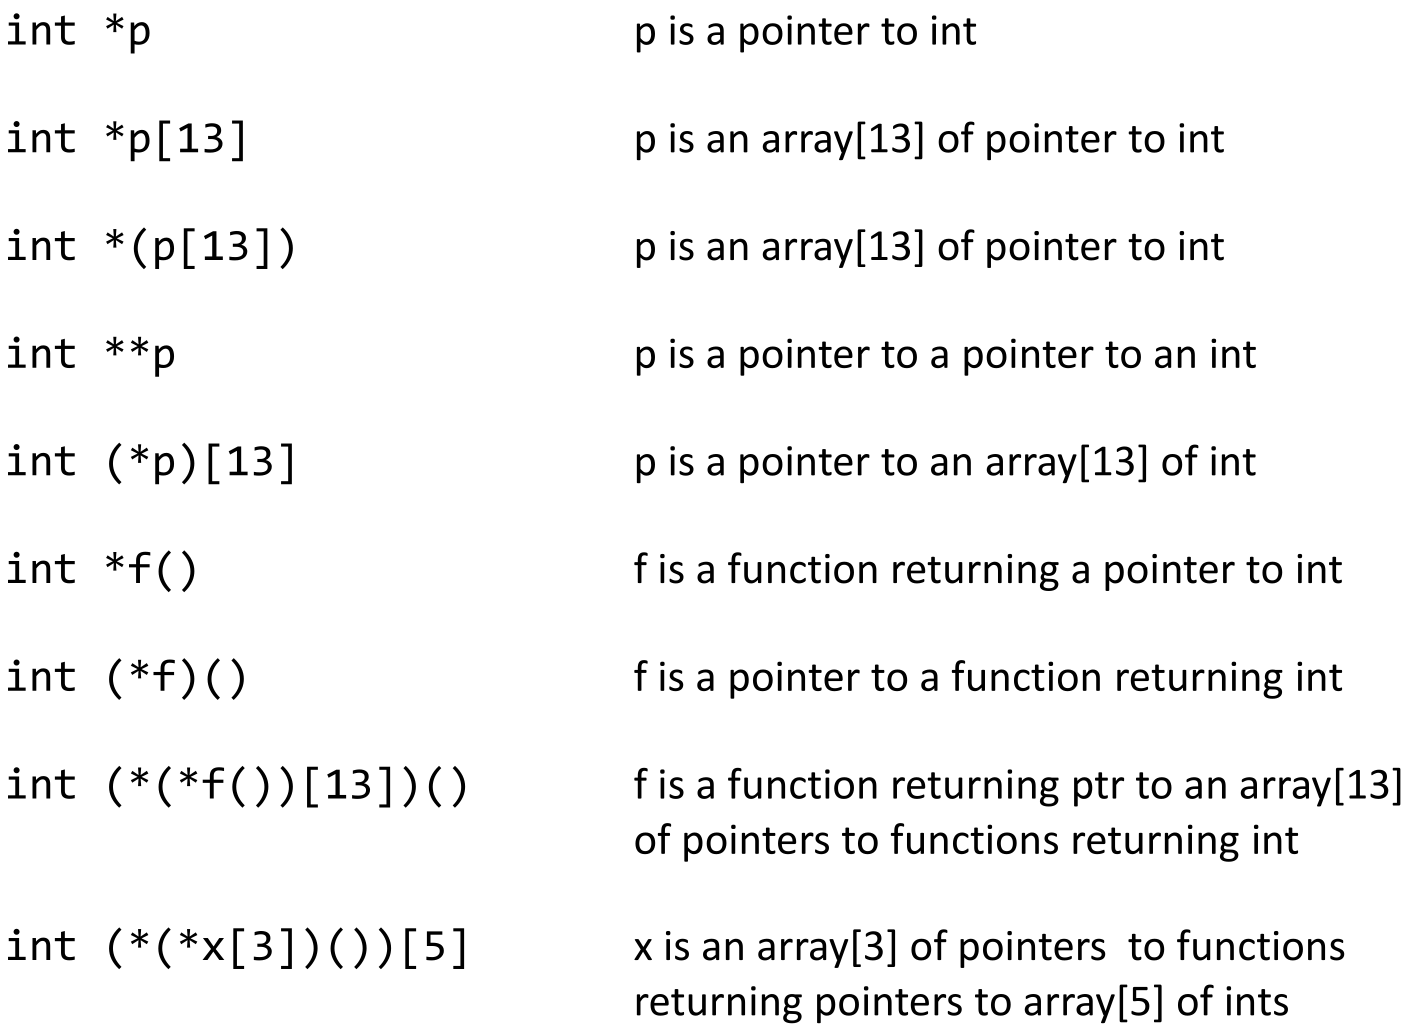
\includegraphics[width=0.8\textwidth]{05_pointerDeclarationEx.png}

    %! TEX root = ./main.tex

\lecture{6}{Week 3}{Dynamic Memory Allocation}

Global variables are allocated statically, meaning that they are allocated when the program is loaded and deallocated when the program exits. Function variables and function parameters are automatically allocated when the function is called and deallocated when the function returns.\\
Often, we want some data to persist across multiple function calls but not for the whole lifetime of a program. Sometimes, the data is also to big to fit on the stack or a function may return a value whose size is unknown to the caller. All these problems an be solved with explicit memory allocation where the program explicitly requests new blocks of memory.

\subsubsection{C Memory API}
\paragraph{Allocation}
\code{void *malloc(unsigned long sz)} allocates a block of size \code{sz} and returns a pointer to the first byte of that memory. Actually, it returns a void pointer, which we then need to convert to our desired type. When null is returned, the memory could not be allocated. Therefore, one should always check if the procedure was successful. 

Typical usage may look as follows:
\begin{lstlisting}
long *arr = (long *)malloc(10 * sizeof(long));
if (arr == NULL) {
    printf("Error");
    return ERRORCODE;
}
arr[0] = 5L; // etc.
\end{lstlisting}

Unlike \code{malloc}, where the initialized memory contains garbage,\code{void *calloc(unsigned long nm, unsigned long sz);} initialized a memory block of size $nm \cdot sz$ containing zeros. It is slightly slower than \code{malloc} but less error-prone and more readable. %Problems with width

\paragraph{Deallocation}
When memory is no longer used, one deallocates it using \code{void free(void *);}, where the argument is the pointer to the first byte of the memory. It is also good practice to null the memory pointer after freeing.

\begin{lstlisting}
long *arr = (long *)malloc(10 * sizeof(long));
if (arr == NULL) {
    printf("Error");
    return ERRORCODE;
}
arr[0] = 5L; // etc.

free(arr);
arr = NULL;
\end{lstlisting}

\paragraph{Resize Memoryblock}
With \code{void *realloc(void *ptr, unsigned long size);} a given block in memory, designated by the pointer to the first memory block, can be resized to the desired size. In most cases the whole memory block is copied to a new location and hence, one should alway use the newly returned address.

\begin{lstlisting}
long *arr = (long *)malloc(10 * sizeof(long));
if (arr == NULL) {
    printf("Error");
    return ERRORCODE;
}

arr = (long *)realloc(arr, 20 * sizeof(long));
if (arr == NULL) {
    printf("Error");
    return ERRORCODE;
}
\end{lstlisting}

\paragraph{size\_t}
Is an unsigned int, e.g. \code{unsigned long} is often used to store memory pointers. They are large enough to hold the size of the largest possible array in memory and are therefore often used to store pointers to memory addresses.

\paragraph{ptrdiff\_t}
Is an unsigned integer of some size and the result of subtracting two pointers. They are used for array loops, size calculations etc.

\subsubsection{Managing the Heap}
The heap is a large pool of unused memory, used for dynamically allocated data structures. \code{malloc/calloc} allocate chunks of memory, \code{free} empties and returns them. In order to know which parts of the heap are used, \code{malloc} maintains bookkeeping data to track allocations.

\paragraph{Memory Corruption}
Memory can corrupt in many different ways:
\begin{itemize}
    \item Assign values past the end of the allocated memory array
    \item Assume \code{malloc} zeroes out memory
    \item Wrong pointer arithmetic
    \item Free unallocated pointer
    \item Double-free same block
    \item Use freed pointer
\end{itemize}

\paragraph{Memory Leaks}
Happen when code fails to deallocated memory that is no longer used. For short-lived programs this is ok, but for long-lived program this is bad.\\
\code{Valgrind} is a tool which helps to detect memory leaks. In the report, \textit{directly loss} means that locations which are directly pointed to are not freed. \textit{Indirect loss} means that the object we point directly to, points to other objects, which are not freed.


\paragraph{Stuctured Data}
A \code{struct} is a C type that contains a set of fields. The tag of the structure is like the name of the structure. To refer to fields of a struct, we use the \code{tag.field} notation, to refer to fields from a pointer to the struct, we can use \code{p\_tag->field} which is the shorthand notation for \code{(*p\_tag).field}. Structs can be initialized by either providing all values at the same time, or by assigning value by value.

\begin{lstlisting}
struct Point {
    int x, y;
};

int main() {
    struct Point p1 = {0, 2};
    struct Point p2;
    p2.x = 4;
    p2.y = 6;

    struct Point *p_p1 = &p1;
    p_p1->x = 5;

    return 0;
}
\end{lstlisting}

When we assign struct types \code{p1 = p2}, the entire content of \code{p2} is copied to \code{p1}. As everything else, a struct is passed by value end hence, the whole struct is copied. Structs can be the return type of a function.\\
When a struct is mixed of fields of different type, the size of the struct may not be equal to the size of the sum of the sizes of the fields, but the struct may get padded. We can print the size of the struct with \code{printf("\%s", sizeof(mystruct));}.

\paragraph{Unions}
They are very similar to \code{struct}, but with the difference that only the most recently assigned value is saved. All other fields cannot be accessed. There is no safety measurements for checking which field is the valid one.

\subsubsection{Type Definitions}
\paragraph{typedef}
They introduce a new type definition and can be used to give a new name to a type. The syntax is \code{typedef type name;}. They are kind of an \textit{alias} for the original type. They allow for writing cleaner code and they are very useful for \code{struct}. For structs we have to add the \code{struct} keyword everytime we want to reference them. Typedef a struct allows to drop this additional keyword and reference it only by the typedef.
\begin{lstlisting}
typedef struct Point {
    int x, y;
} Point_t;

int main() {
    Point_t p1 = {0, 2};
    Point_t p2;

    return 0;
}
\end{lstlisting}

Typedef can also be useful to build up complex declarations.

\paragraph{Namespaces}
A namespace is a set of names of objects in a system. They allow the disambiguate different objects with same name. C has different namespaces for:
\begin{enumerate}
    \item Label names for \code{goto}
    \item Tags of \code{struct}, \code{union}, \code{enum}
    \item Member names, for each \code{struct}, \code{union}, \code{enum}. I.e. each \code{struct} has a different namespace.
    \item Everything else, including \code{typedef}
\end{enumerate}

\subsubsection{Dynamic Data Structures}
In C we can implement dynamic data structures, like linked-lists, as we are used to in other languages.

\subsubsection{Generic Data Structures}
When we want to let the user choose the type stored in the data structure, we can store in each node a generic pointer \code{void *element} instead of a fixed type. Clients can convert their specific type to \code{void *} before pushing it to the data structure.

    %! TEX root = ./main.tex

\lecture{07}{Week 4}{Wrapping up C}

\paragraph{C Preprocessor}
The C preprocessor (cpp) is not part of the language buts sits on top of it.

\paragraph{Include}
\code{\#include} is used to include header files inline in the source code. They provide a basic mechanism for for defining APIs.\\
Header files are either system header files, which are included using \code{<systemHeader>}, or own header files, included using \code{"ownHeader"}. We do not need to provide a path to the file, but the preprocessor will look at certain dedicated paths for the appropriate files.\\
It is important to \textbf{not} include a file twice. Also one should never include \code{.c} files.

\paragraph{Macros}
Macros provide token-based text substitution. A macro is defined using \code{\#define foo bar}. Any appearance of \code{foo} in the code is replaced with \code{bar}. Since macros are purely textual, we can use them for \textit{expressions} too. E.g. \code{\#define inc(x) (x + 1)} will replace \code{inc(1)} with \code{(1 + 1)}.\\
An undefined, or a defined macro which was removed using \code{\#undef foo} will evaluate to $1$ which evaluates to true in an expression.\\
Macros can span multiple lines and contains \textit{complex} structures by adding a backslash to the end of the line. The problem we may encounter with macros which represent a expression is that adding a semicolon after the term which gets replaced by the macro, results in two semicolons (if there is one in our macro too). When using the trick of \textit{Semicolon Swallowing}, we put our macro block inside a \code{do {ourMacro} while(0)} block. Adding a semicolon after the macro will no longer result in an error. The compiler removes the loop anyways.\\
An advantage of macros is to prevent overhead by inlining. But the compiler can do that by itself nowadays.

\paragraph{Conditionals}
Conditionals are useful to take different action at the build time. Preprocessors support conditionals of the form:
\begin{lstlisting}
\#if expression1
    (text1)
\#elif expression2
    (text2)
\#else
    (text3)
\#endif
\end{lstlisting}

Important is that expressions must be macros and literals only!

The conditional \code{\#ifdef foo} and \code{\#ifndef bar} evaluate to true or false depending whether the macro is defined or not. This is a shorthand for \code{\#if defined(foo)} and \code{\#if !defined(bar)}.

\subsubsection{Modularity}
A module is a self-contained piece of a larger program. It consists of an externally visible part, containing functions, typedefs, global variables, cpp macros (they define the module's interface) and of internal functions, types, variables which are hidden from the client.

\paragraph{Declaration vs Definition}
C differentiates between declaration and definition. A declaration is like the definition but without the body. Structs are declarations and cannot be defined.\\
A \textit{compilation unit} is a C source file and everything it includes. The compilation unit defines the visibility of definitions.\\
When we want to access a definition from another compilation unit (or the same) we prepend the declaration with \code{extern}. When prepending the declaration by \code{static}, this definition is only visible inside this compilation unit and cannot be accessed from the outside using \code{extern}.

\paragraph{Global Variables}
Global variables are also declared and the visibility can be controlled using \code{extern} as described above.

\paragraph{Header Files}
Header files specify interfaces and should not contain declarations (structs are definitions and not declarations). The module \code{foo} has the interface specified in \code{foo.h} and all clients of \code{foo} are required to include \code{\#include "foo.h"}. The implementation of \code{foo} is typically in the \code{foo.c}, which also must include \code{foo}. This source file ought not contain external declarations but only definitions and internal declarations.\\
The naming \code{foo.c} and \code{foo.h} is just a convention which the compiler does not care about (i.e. they can have different names). For the execution simple the name of the definition matter.

\paragraph{CPP Convention}
One should never include the same header file twice or redeclare macros. Therefore, it is convenient to have a mechanism which prevents this. The following boilerplate ensures that the header file containing the code cannot be imported twice.

\begin{lstlisting}
\#ifndef __FILE_H_
\#define __FILE_H_
(macros, headers)
\#endif
\end{lstlisting}

\code{\_\_FILE\_H\_} is the name if the program (or something like that).

\subsubsection{Function Pointers}
Function pointers are pointers for functions. For example in \code{int (*funct)(int *, char);} \code{func} is a pointer to a function which takes two arguments, a pointer to int and a char. The return value of the function is int. Function pointers are rare in OOP languages, but they are sometimes referenced as \textit{delegates} or \textit{agents}.\\
Function pointers are very fundamental for a lot of techniques in system code. They allow for example to write \textit{object oriented like code} by having a struct of variables and functionpointers (sometimes called \textit{vtable}). This method does not provide any protection or hiding but does provide the benefit of reusability.

\subsubsection{Assertions}
Assertions evaluate an expression at runtime and crash the program if evaluated to false. In that case they print \code{"<filename>:<linenumber> <functionname>: Assertion <assertionexpression> failed."} and then abort.\\
Assertions are macros and using the compile flag \code{-DNDEBUG} they can be removed.

\subsubsection{goto}
Goto should be be used, except for:
\begin{itemize}
    \item Early termination of nested loops. But we may also put this in a dedicated function and return.
    \item Cleanup code. Like transactional memory, when one step fails, undo all previous steps. Depending on which stage failed, we need to undo a different number of steps.
\end{itemize}

The second usecase is visualized here:

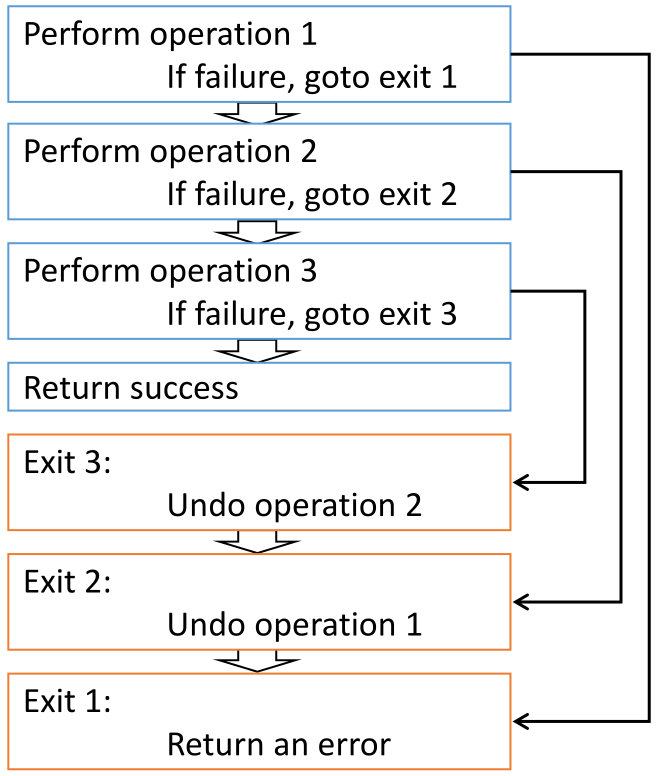
\includegraphics[width=0.8\textwidth]{07_CleanupCode.png}

\subsubsection{setjmp() and longjmp()}
They are imported with \code{<setjmp.h>}. The function \verb+int setjmp(jmp_buf env)+ saves the current stack state and environment to \code{env}. Then it returns $0$.

The function \verb+void longjmp(jmp_buf env, int val)+ takes a buffer of \code{setjmp} and causes the \code{setjmp} to return again the value of \code{val} or $1$ if $val = 0$. For each \code{setjmp}, this can only be done once and also only as long as the function containing \code{setjmp} has not returned.\\
This construct is very unique to C.

It can be used like:

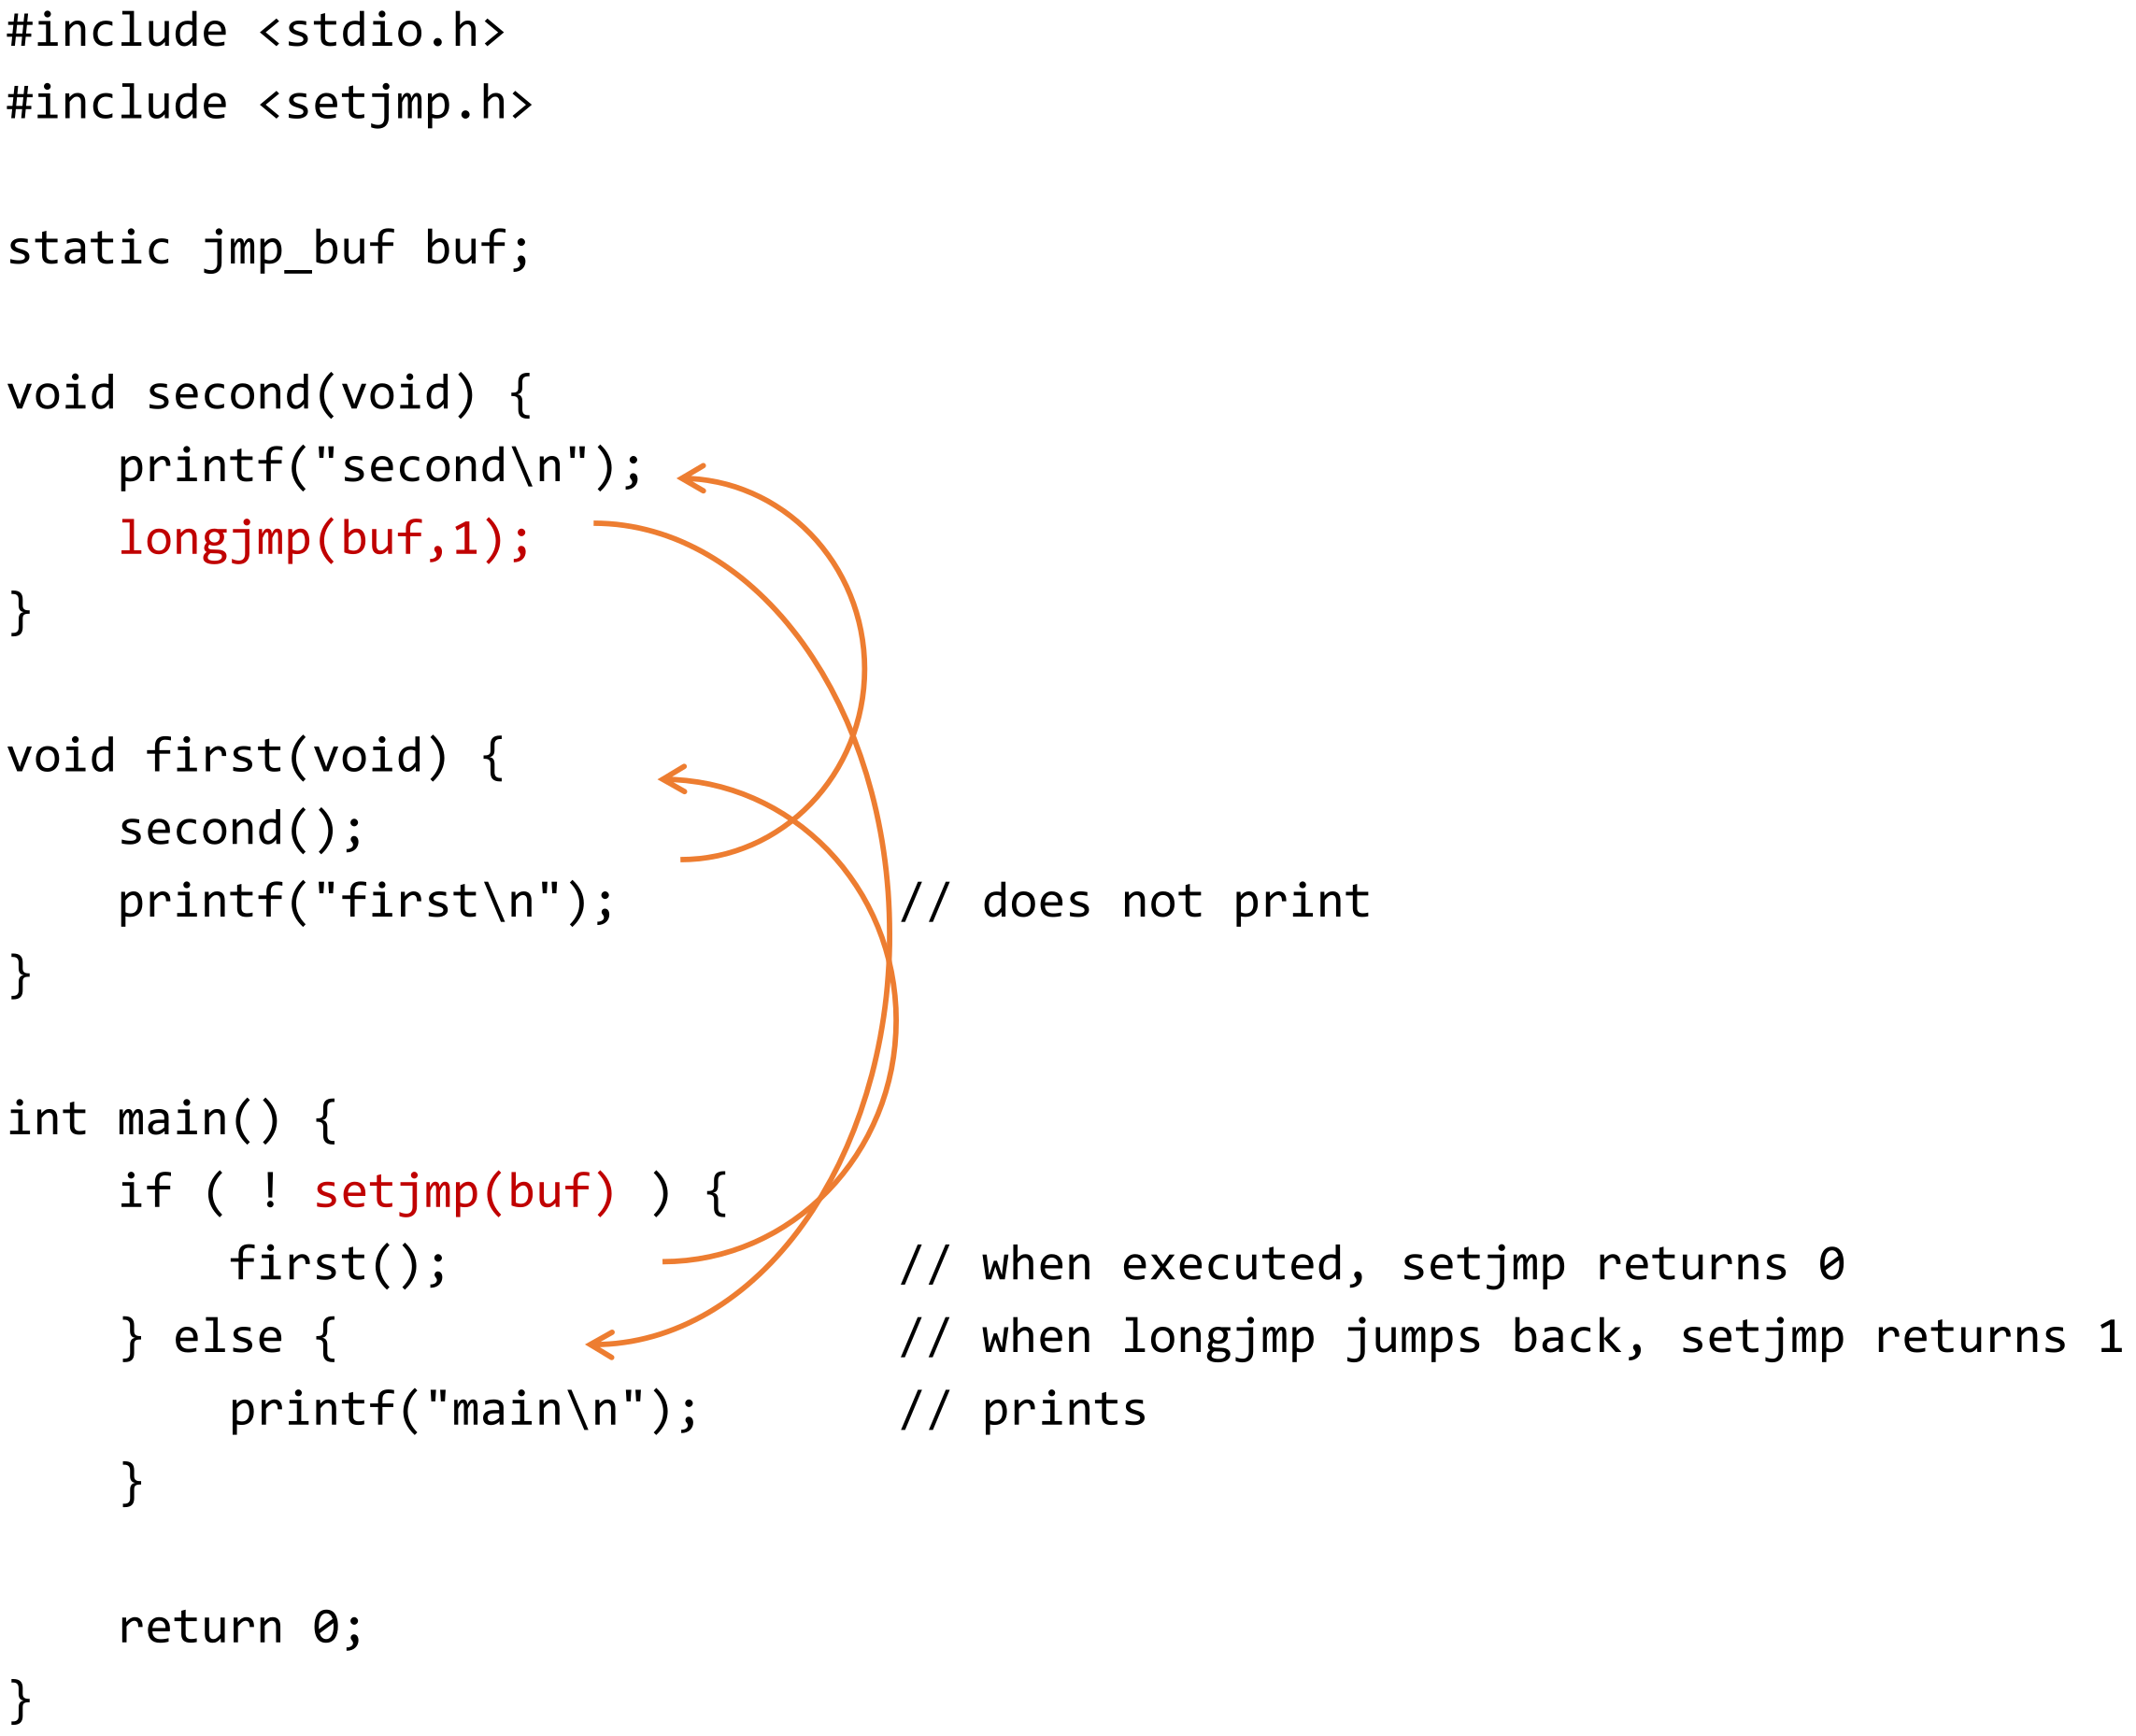
\includegraphics[width=0.8\textwidth]{07_setjump.png}

\subsubsection{Coroutine}
Coroutines are methods which are both at the top of the stack at the same times. Both routines should be able to call eachother to transfer e.g. data. They look similar to threads but they are not. In essence they allow dynamically switching between functions.

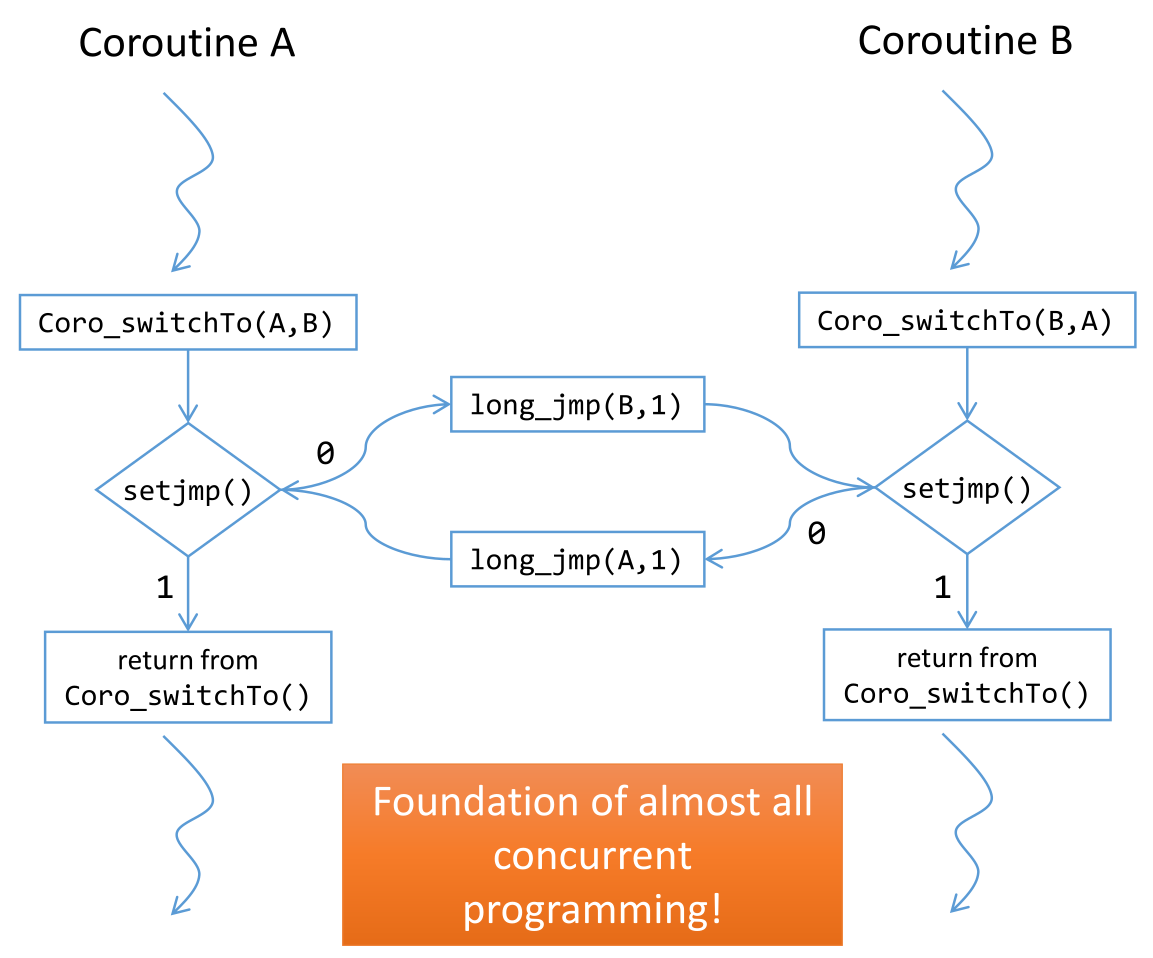
\includegraphics[width=0.8\textwidth]{07_coroutine.png}

Coroutines are completely based on \code{setjmp} and \code{longjmp}.

Coroutines are sometimes called \textit{Lightweight threads}, \textit{Protothreads}, \textit{Cooperative mtultitasking}... Thread based programming is based on this schema and we can make coroutines look like threads by dynamically switching into different functions. But there is no concurrently and no parallelism.

Sidenote; The comma \verb+a() , b()+ is an operator which takes two statements. Both are evaluated, but only the second one is returned.

    %! TEX root = ./master.tex

\lecture{08}{Week 4}{Implementing Dynamic Memory Allocation}


Sidenote: A Runtime allows a programming language to use C libraries. C does not have a runtime, therefore it is well suites for e.g. OS programming.

The OS allocates memory to the C program in pages. But we often only need a few bytes. A memory allocator is a interface which sits between the application and the memory and gives out memory blocks to applications. A block is a continuous range of bytes of any size.\\
\code{malloc} is such a dynamic memory allocator

\paragraph{Address Space}
The address space is split into multiple parts. The NULL pointer is at address $0x00000000$ and contains nothing. On top of it, at $0x00000008$ is the \textit{Text}. This section contains the machine code of our functions. On top of it is the \textit{Data} section, where global variables and parameters (?) are stored. On top of all that is the heap, which grows upwards. At the top at $0xFFFFFFFF$ is the stack, which grown downwards. Functions of libraries, like \code{malloc} are dynamically linked and the address is determined at runtime. Addresses in the heap are not allocated linearly, but in some different fashion.

\paragraph{Explicit Memory Allocation}
Allocation and free is done manually by the user. All operations appear in the program source. After allocation, there is a point of time, from when on the object must be accessible. There is another point in time, before which the data object cannot be freed.

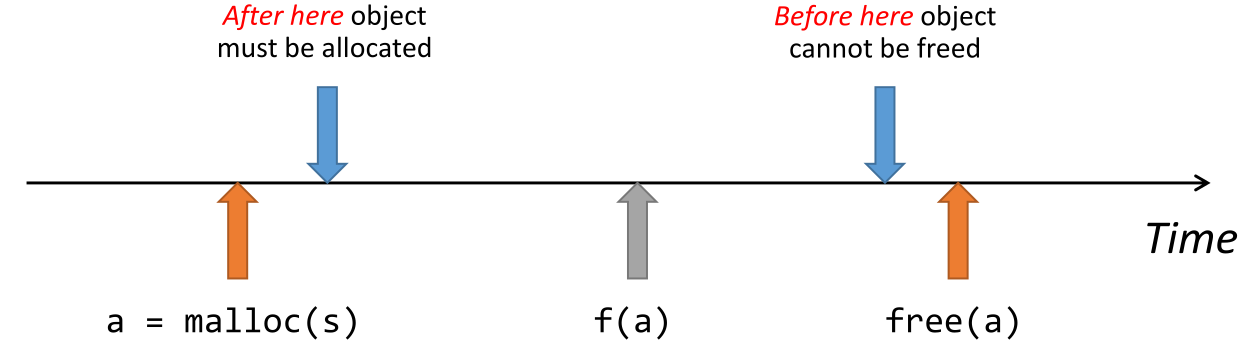
\includegraphics[width=0.8\textwidth]{08_memoryallocationcycle.png}

\paragraph{Implicit Memory Allocation}
The user allocates memory by creating new objects. But they are implicitly deallocated by a \textit{Garbage Collector}. After a new object is initialized, there is some point in time, where the allocation must be finished and the object must be available. There is again a point in time before which the object cannot be freed. Once the object becomes unreachable, meaning we do not habe a reference to the abject anymore (this does only work because such languages do not support pointers), the garbage collector frees the memory.

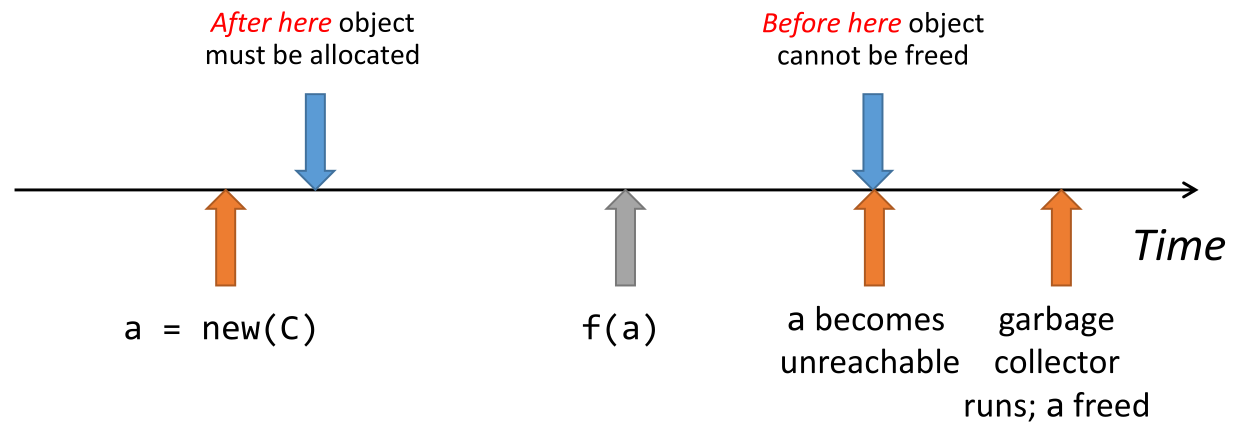
\includegraphics[width=0.8\textwidth]{08_garbagecollectedcycle.png}

\paragraph{Compiler Supported Memory Allocation}
The compiler proves from which point on a object must exist, and from which point on it is no longer required. This way the compiler decides when to allocate and deallocate occur. This makes a language extremely fast.

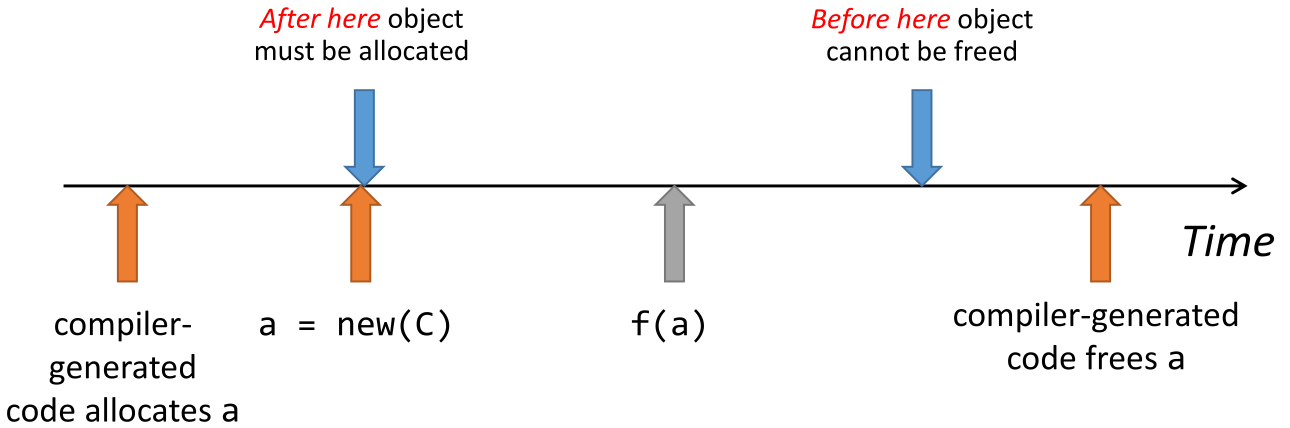
\includegraphics[width=0.8\textwidth]{08_compilersupportcycle.png}

All memory allocations use explicit allocation under the hood, therefore it is crucial to have a good understanding about it.

\subsubsection{The Problem}
In this lecture we assume that memory is word addressed. This has the advantage that each word can hold a pointer.

\paragraph{Constraints}
One of the difficulties is that in a program we can issue arbitrary sequences of allocate and deallocate. Memory allocators cannot control the number or size of allocated block and obviously the y can only allocate free parts of the memory. Since they must respond immediately, they also have to time to reorder or buffer requests. Blocks must also be aligned to satisfy external requirements (8 byte alignment for GNU \code{malloc}). This means that the payload (/block) must always start at an alignment line (for better CPU performance). One a block is allocated, this block cannot be moved or changes anymore.

\paragraph{Performance Goal}
Given a sequence of allocations and deallocations, we want to maximize the \textit{throughput} as well as the \textit{peak memory utilization}. These goals are conflicting by nature.

\subparagraph{Throughput}
The throughput is the number of requests per unit time. The goal is to perform allocations and deallocation operations in $O(1)$.

\subparagraph{Peak Memory Utilization}
The peak memory utilization defines how efficiently we use the available memory.

To measure the peak memory utilization we define for some sequence of allocations/deallocation $R_0, R_1 \dots R_k, \dots R_{n-1}$

\begin{description}
    \item[Aggregate playload $P_k$:] The sum of currently allocated payloads (the difference between all \code{malloc(p\_i)} and all \code{free(p\_j)}). Where a payload of $p$ bytes is generated by \code{malloc(p)}.
    \item[Current heap size $H_k$:] Assume $H_k$ is monotonically increasing.
    \item[Peak memory utilisation after $k$ requests $U_k$:] $(\text{max}_{i<k} P_i) / H_k$ 
\end{description}

\paragraph{Fragmentation}
Fragmentation may cause poor memory utilization. The two types of fragmentation are:

\begin{description}
    \item[Interlan Fragmentation:] For a given block where the payload is smaller than the block size
        the payload is padded by unused unused space. Another cause is bookkeeping information, like start and end tags, are added.
    \item[External Fragmentation:] When there is enough free space on the heap, but not as a single free block.
\end{description}

While internal fragmentation is predictable and easy to measure, external fragmentation depends on the pattern of requests und therefore is difficult to predict and measure.

\paragraph{Size of a Memory Block}
In order that \code{free} knows how large the block of the memory to free is, \code{malloc} keeps track of the size of a memory block, by storing the size in the first word of the newly created memory block. The pointer it returns actually points on the second word.

\subsubsection{Keeping Track of Free Block}
The key policies for memory allocators are Placement policy (wo do we find the block to use), Splitting policy (how do we split blocks which are too large) and Coalescing policy (how do we merge free blocks).

\paragraph{Implicit Free List}
For each block we need to know its size, as well as whether it is allocated or not. We store all these information in the first word of block. The allocated flag is actually the least signification bit of the length. This introduces some internal fragmentation (because the length up rounded up), but it can be neglected. Especial also since due to the alignment of block, some of the lower-order address bits are often anyways always $0$.

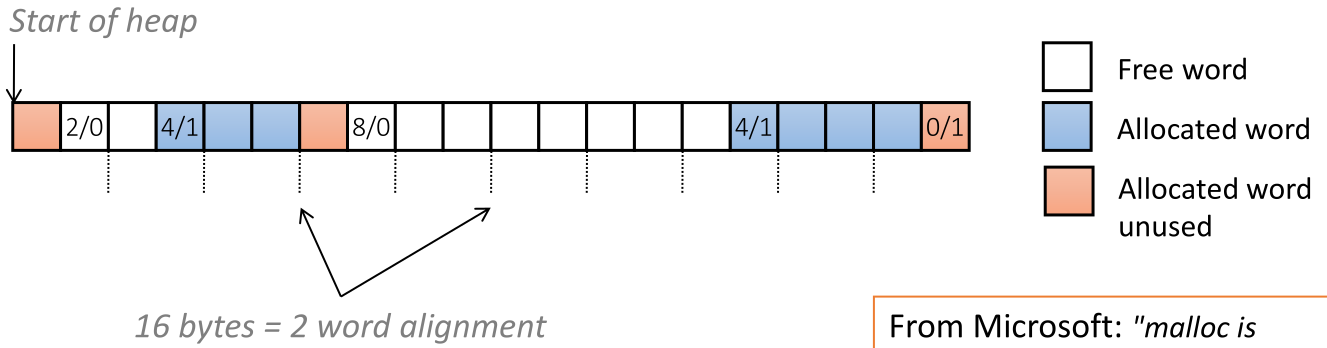
\includegraphics[width=0.8\textwidth]{08_implicit_free_list.png}

Due to alignment restrictions, the first word of the heap is never allocated.

\subparagraph{Finding a free block}
In order to find a free block, we iterate all blocks, starting from the first black, till we find the first free block which confirms to our space requirements. This approach takes linear time in the number of total blocks. In practice, we end up with many small blocks at the beginning of the list.

There are slight variations from this method:
\begin{description}
    \item[First Fit:] As described, takes the first suitable block from the beginning of the list
    \item[Next Fit:] As first fit, but does not start iteration from the beginning, but where it found a suitable free block the last time. This should be faster but may introduce more fragmentation.
    \item[Best Fit:] Iterates the whole list and takes the best fit (the one with the fewest bits left over). This keeps fragmentation small but is slower.
\end{description}

Often, we have to split an free block to not waste too much space.

\subparagraph{Freeing a block and coalescing}
When a block is freed, we do not want that a large free block is actually split in multiple small ones. Therefore, sequential free blocks should be merged into one large free block. This procedure is refereed to as \textit{coalescing}.\\
We can easily skip following free blocks by simple increasing the length of the freed block. This does logically ignore the length entry of the following free block.\\
In order to coalesce with previous block, we actually need to add an end tag/footer to each block, wich contains, equally as the header tag, the length of the block and a empty flag. This way we can coalesce previous blocks too by looking at the last word of the previous head.\\
Coalescing can be done in constant time for all possible allocated/unallocated scenarios.

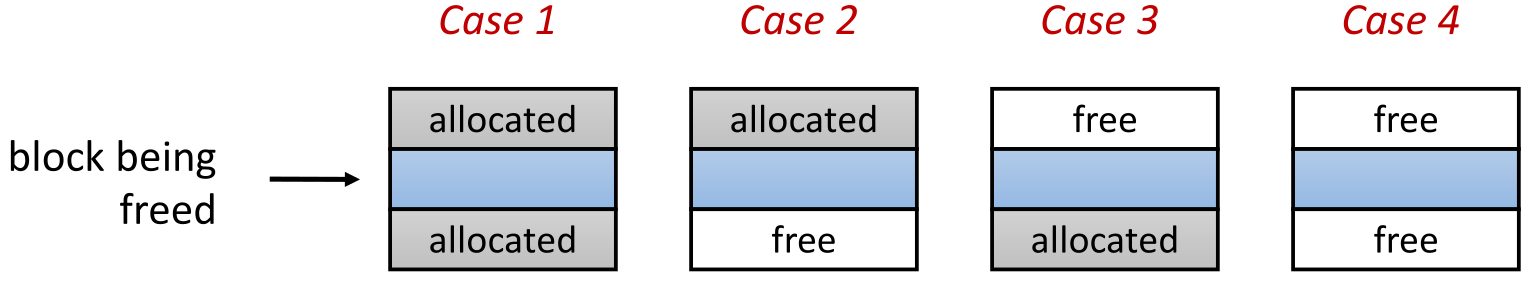
\includegraphics[width=0.8\textwidth]{08_coalecationsettings.png}

The additional end tag leads to internal fragmentation. 

\paragraph{Explicit free lists}
As the implicit list, it has an start tag and an end tag for coalescing. But in order to find free blocks, a pointer to the previous free block is stored in the first word of the payload area and in the second word, a pointer to the previous free block.

\subparagraph{Finding a free block}
We iterate our list and look for a valid block. In order to allocate a choose block we simple change the pointer pointing to our block.

\subparagraph{Freeing a block and coalescing}
In order to free a block simply add it to our list. There are multiple insertion policies which determine were in the list the new block is inserted:

\begin{description}
    \item[LIFO policy:] We insert the new block at the beginning of the list. This is simple to implement and has constant time. However, fragmentation may be worse.
    \item[Address-ordered policy:] We insert the blocks so that the address of the blocks are ordered. This requires search to find the desired location, but in turn, fragmentation should be better.
\end{description}

This method is faster than implicit free list, since the required time is linear in the number of free blocks.

\paragraph{Segregated free list}
Similar to the explicit free list. But in contrast to that, we keep separate lists blocks of different size. Most of the time, small blocks are allocated, hence this gives very good performance.

\subparagraph{Finding a free block}
To allocate a block of size $n$ we search the list of blocks of size $m > n$. On success, we split the block (if required) and place the fragment on the appropriate list. We to to higher-level classes, till we have found a suitable block. If there is no such block, we request a new memory block from the OS. 

\subparagraph{Freeing a block and coalescing}
We coalesce the block and put in on the appropriate list.

The advantage of this method is the high throughput as well as the better memory utilisation.

Most allocated blocks are rather small. Segregated list give very good performance. Large blocks are only occasionally assigned. Many systems use this method.

    %! TEX root = ./master.tex

\lecture{09}{Week 5}{Basic x86 Architecture}

\subsubsection{Instruction Set Architecture}
The term \textit{Architecture} or \textit{Instruction Set Architecture (ISA)} is very vaguely defended in computer science. It kind of is a building plan for a CPU and it is what one should understand in order to write assembly code. The \textit{Microarchitecture} is in contrast, the implementation of the architecture. A good knowledge of the microarchitecture, on top of the ISA, allows to write very fast, but hardware specific code.\\
The first real architecture was IBM 360. 

\paragraph{CISC: Complex Instruction Set}
Their philosophy is to add hardware based instruction for often used functionality. So for example, a CISC CPU may have a sorting instruction. This was the dominant style through mid-80's. It was a stack oriented instruction set, meaning a set was used to pass arguments, save PC. Instructions were rather complex and for example one could access memory directly from arithmetic instructions. Conditional codes were used.

\paragraph{RISC: Reduced Instruction Set}
This is a ISA which which tried to keep instructions as simple as possible, and hence, was a direct contrast to the CISC. Many simple instructions may be required to replace a single CISC. But in turn, they can be executed on small and fast hardware. It is a register-oriented instruction set. Memory access was limited to dedicated load/store operations and it has no conditional code.\\
RISC is quite different from x86, they tried to strip away everything and make the hardware very simple.

\paragraph{MIPS}
MIPS is a RISC ISA. It has very standardized instructions which all have the same bite length and take approximately the same amount of time to execute. All operations act on registers except load and store. This makes the circuit simple and faster.\\
Most numbers in computers are zero. Therefore, it is also handy to have a zero register, as MIPS has.

\paragraph{CISC vs. RISC}
This is a very old debate and both philosophies have their advantages and disadvantages. Code for CISC is easier to compile and has a smaller code size. RISC was better optimized for compilers and runs faster with simpler chip design.

\paragraph{CISC vs. RISC Today}
This debate is over and there is no winner. Complex hardware got cheaper to do, so RISC packed more advanced features on their CPU which CISC decoded their complex instruction into simpler microinstructions which were faster to execute. Today, there is almost no difference between CISC and RISC.\\
Performance is not really an issue today. Today a successfully ISA is one which is compatible with existing code, licensing, security etc.

\subsubsection{x86 History}
\paragraph{Intel x86}
A very successful chip was the $8086$, which was a $16$ bit processor and which was introduced in 1978. It has many revisions and was also adapted to a $32$ version, with the $80386$ in 1985. This ISA was named IA32 and recent code can still be run on this CPUs. They tried to radically shift from ia32 to ia64, however they failed because their Itanium architecture were very slow executing existing code, but only fast when writing new, code.\\
$8$ months after AMD released their x86-64, Intel released a compatible version ISA called EM64T (later renamed to Intel 64), wich was almost identical to x86-64. Their first 64 bit CPU was the Pentium 4F in 2005.\\
From 2012 on, when the i7 was released, this Architecture was kept the same and many features were added.

\paragraph{AMD x86}
AMD is a rival of Intel and normally, they produces a bit slower but cheaper CPUs with less features. However, they have hired many top engineers and compete with Intel. Thanks to this, they have developed the Opteron, the first 64bit CPU to x86-64 (now called AMD64) based.

\subsubsection{Basics of Machine Code}
There are two common ways to write x86 assemly. The first one is the AT\&T syntax which is common to Unix and which we will use in this course, and there is the Intel syntax, which Windows uses.

\paragraph{Compiling C to Assembly}
In order to compile to so assembly, we can use \code{gcc -O -S code.c}, where \code{-S} is the flag to get assembly code. This produces a file called \code{code.s}.

\paragraph{Assembly Data Types}
Assembly has very little concerning semantics. The integers, containing data values and untyped pointer addresses have either $1$, $2$, $4$ or $8$ bytes length. Floating point data has $4$, $8$ or $10$. Besides that, there is nothing, no arrays, no structs...

\paragraph{Assembly Code Operations}
We can perform arithmetic operations on registers or memory data. We can move data between registers and memory and there are conditional and unconditional branches.

\paragraph{Object Code}
In object code \code{.o}, the assembly code \code{.s} ins binary encoded. This is done by the assembler. In x86, instructions have variable length (unlike in MIPS).j

\paragraph{Disassembling Object Code}
This is the process of generating assembly code \code{.s} from object code \code{.o}. Disassembled code is not identical to the original assembly code, since object code does not have all program information, since assembly has some \textit{high level} usercode, like jump target names etc. A disassembler works by examining bytes and reconstructing the assembly instructions.\\
A disassembler is \code{objdump -d <file>} and it works for \code{a.out} as well as \code{.o} files. Alternatively, one can use the \code{gdb} debugger for disassembling. This tool has a little cumbersome syntax.

\subsubsection{x86 Architecture}
\paragraph{8086}
This $16$ bit CPU had $10$ registers where $6$ of them were for general purpose. Although, even the general purpose registers wer designed for a specific purpose. This processor is the predecessor of the 8008, which was a $8$ bit processor wich has $4$ registers. The 8086 is actually an extension of that and therefore $4$ of the general purpose registers could access in high/low (access top $4$ respectively bottom $4$ bits separately).

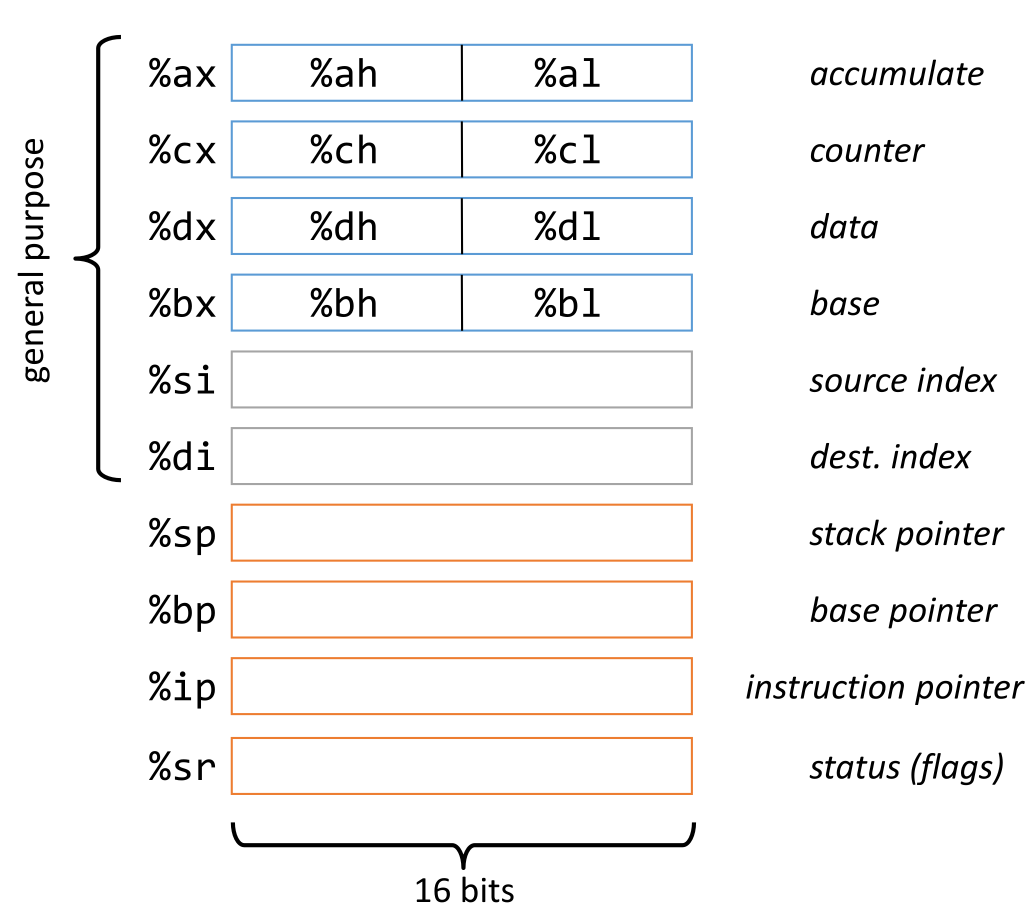
\includegraphics[width=0.8\textwidth]{09_8086.png}

\paragraph{80386 (ia32)}
This ISA is again an extension of the 8086. It extends all registers to $32$ bits, but still allows access to the lower $16$ bits and the high/low bits. The name for the full $32$ bit register are simple the original register names with an appended e.

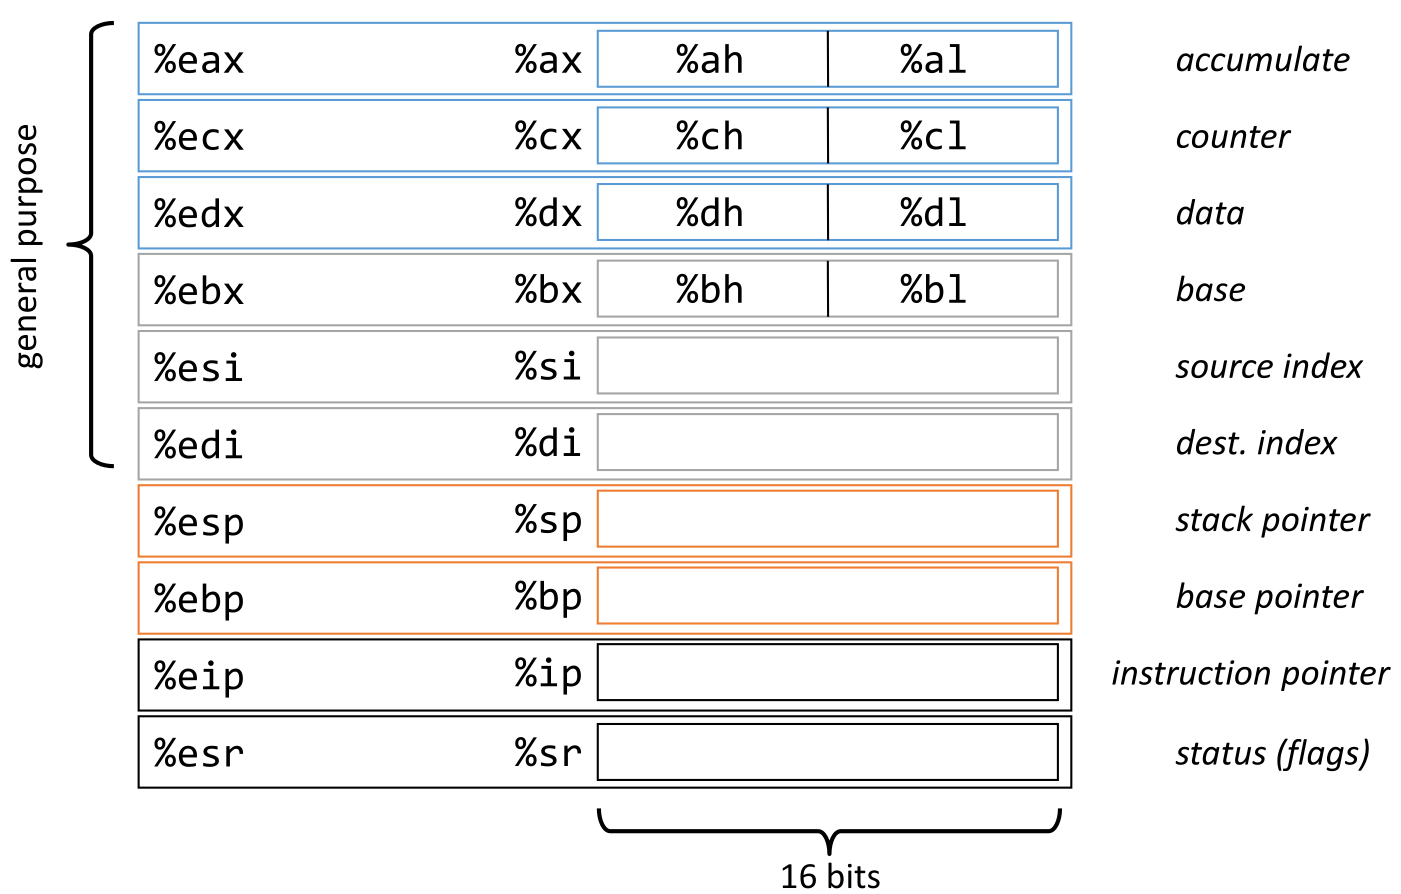
\includegraphics[width=0.8\textwidth]{09_80386.png}

\paragraph{x86-64}
In this ISA they have extended the $32$ bit registers to $64$ and doubled the number of general purpose registers compared to the ia32 (have a total of $16$). Again, they allow to access the lower $32$ (but not $16$) bits and the register name of ia32 was extended by prepending an r. Even though some registers still have some special name, we can actually use them for whatever we want.

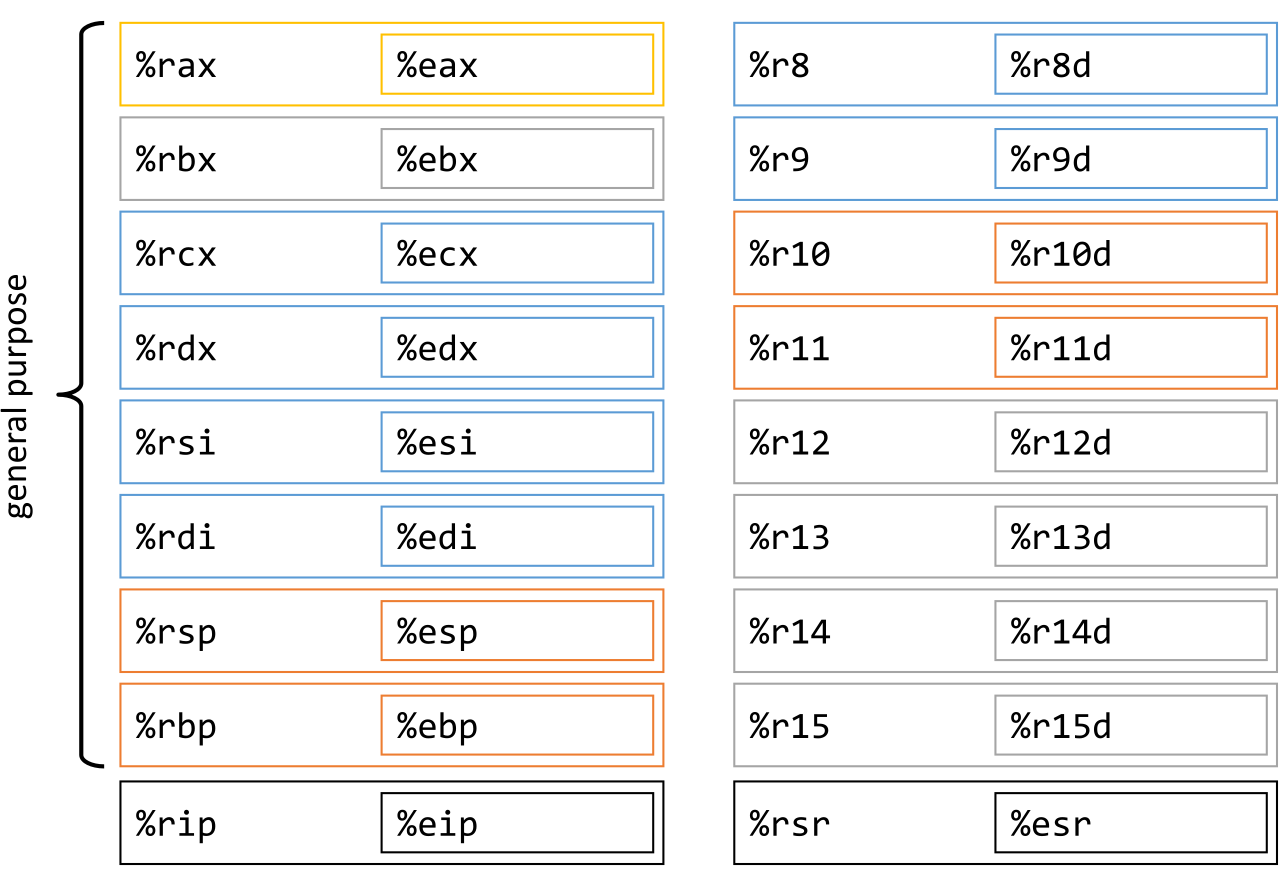
\includegraphics[width=0.8\textwidth]{09_x86-64.png}

\paragraph{Moving Data}
There are four flavours of the move instruction \code{movx Source, Dest}.
\begin{description}
    \item[movq:] move $8$-byte \textit{quad word}
    \item[movl:] move $4$-byte \textit{long word}
    \item[movw:] move $2$-byte \textit{word}
    \item[movb:] move $1$-byte \textit{byte}
\end{description}

There are three operand types.
\begin{description}
    \item[Immediate:] Constant integer in decimal or hexadecimal prepended by a $\$$ sign. The size can be $1$, $2$, $4$ or $8$ bytes.
    \item[Register:] Registers are referred by their name. There are general and special purpose registers.
    \item[Memory:] The general access mode is \code{D(Rb, Ri, S)} which is leads to a access of \code{Mem[Reg[Rb] + S * Reg[Ri] + D]}
        \begin{description}
            \item[D:] Constant displacement of size $1$, $2$ or $4$ bytes
            \item[Rb:] Base register; any of the 16 registers
            \item[Ri:] Index register; any of the registers except \code{\%rsp}
            \item[S:] Scale; any of $1$, $2$, $4$ or $8$. It is used for array access for arrays of certain type.
        \end{description}
\end{description}

Not all combinations of source and destination are available. So it is not possible to transfer data from memory to memory in one instruction.

\paragraph{Address Computation Instruction}
The command \code{lea Src, Dest} does not move any data, but rather calculates the address given by the address mode passed by \code{Src} and writes the address to \code{Dest}. This is useful when we need to compute an address without memory memory access, e.g. when creating a pointer. But it can also be used for general arithmetic.

The reason being is that the address calculation requires lot of hardware. Therefore, it does also make sense to use it for arithmetic.

    %! TEX root = ./maimain.tex

\lecture{10}{Week 5}{Basic x86 Architecture and C Control Flow}

\subsubsection{x86 Integer Arithmetic}

\paragraph{Some Arithmetic Operations}
Important two-operand instructions:

\begin{tabular}{l l}
    \code{addl} & $Dest = Dest + Src$\\
    \code{subl} & $Dest = Dest - Src$\\
    \code{imull} & $Dest = Dest * Src$\\
    \code{sall} & $Dest = Dest << Src$\\
    \code{sarl} & $Dest = Dest >> Src$\\
    \code{shrl} & $Dest = Dest >> Src$\\
    \code{xorl} & $Dest = Dest\ \hat{}\ Src$\\
    \code{andl} & $Dest = Dest \& Src$\\
    \code{orl} & $Dest = Dest | Src$
\end{tabular}

There is no difference between arithmetic and logic shift left, and hence, the instructions \code{sall} and \code{shll} are equivalent.

Two-operand instructions store the result of the calculation in one of the operands. There is not separate register. This is a limitation which stems from the early days where registers were rar but nowadays, where registers are actually stored in a register file with +200 resists which is is no longer an issue. (The name of a regster is just a temporary reference to an entry of the register file)

All operations act on the binary numbers and there is no notion of signed or unsigned integers. That is because it does not make any difference for the computation!

Important one operand instructions:

\begin{tabular}{l l}
    \code{incl} & $Dest = Dest + 1$\\
    \code{decl} & $Dest = Dest - 1$\\
    \code{negl} & $Dest = -Dest$\\
    \code{notl} & $Dest = \tilde{} Dest$
\end{tabular}

\paragraph{\code{lea} for Arithmetic Expressions}
The compiler clever and makes us of \code{lea} for arithmetic instructions. This is especially powerful when replacing a multiplication by \code{lea} and shifts.

The C compiler is better in assembly than we humans :)

There is again a version for different sized: \code{leal} etc.

\subsubsection{Condition Codes}
Condition codes are extra bits, like one-bit registers. But they are packed into the status register. They provide us extra information about executed operations.

They have names and they are set (implicitly) during arithmetic instructions (but \textbf{not} by \code{lea}):
\begin{description}
    \item[CF:] Carry Flag (for unsigned)
        \begin{itemize}
            \item Set if carry out of most significant bit
            \item i.e unsigned overflow
        \end{itemize}
    \item[ZF:] Zero Flag
        \begin{itemize}
            \item Set if result is equal to $0$
        \end{itemize}
    \item[SF:] Sign Flag (for signed)
        \begin{itemize}
            \item Set equal the most significant bit
            \item i.e. if interpreted as signed, the result is negative
        \end{itemize}
    \item[OF:] Overflow Flag (for signed)
        \begin{itemize}
            \item Set to \code{( a > 0 \&\& b > 0 \&\& t < 0) || (a < 0 \&\& b < 0 \&\& t >= 0)}
            \item i.e. if interpreted as signed, the results overflows
        \end{itemize}
\end{description}

Condition codes can also be set explicitly using the \code{cmpl/cmpq Src2, Src1} instruction. This instruction computes i.e. \code{Src1 - Src2} and sets the conditional flags (but does not store the result of the computation).

The second instruction to set the condition codes explicitly is \code{testl/testq Src2, Src1}. It computes \code{Src1 \& Src2}, sets the condition codes but again, not the result. This instruction is very useful when one instruction is a mask.

\paragraph{Read Condition Codes}
The \code{SetX Dest} instruction computes an expression based on the current flags and writes that to the low-byte of a register. There are the following flavours:

\begin{tabular}{l l l}
    \code{sete}  & $ZF$                                     & Equal/Zero\\
    \code{setne} & $\tilde{} ZF$                            & Not Equal/Not Zero\\
    \code{sets}  & $SF$                                     & Negative\\
    \code{setns} & $\tilde{} SF$                            & Non-Negative\\
    \code{setg}   & $\tilde{} (SF\ \hat{}\ OF) \&\ \tilde{} ZF$ & Greater (Signed)\\
    \code{setge}   & $\tilde{} (SF\ \hat{}\ OF)$                & Greater or Equal (Signed)\\
    \code{setl}   & $(SF\ \hat{}\ OF)$                         & Less (Signed)\\
    \code{setle}   & $(SF\ \hat{}\ OF) | ZF$                    & Less or Equal (Signed)\\
    \code{seta}   & $\tilde{} CF \&\ \tilde{} ZF$             & Above (Unsigned)\\
    \code{setb}   & $CF$                                     & Below (Unsigned)\\
\end{tabular}

$32$ bit instructions set the higher-order bit, of e.g. \code{\%rax} to the same value when writing to \code{\%eax}. The \code{setX} operations are not $32$ bit instructions and therefore do not modify the higher-order bytes but only sets the least significant byte! \code{xor} is a cheap way to set a register to $0$. So with the combination of \code{xor} and \code{setX} we can move a certain flag wo any register we want.

\code{movzbl} moves a byte to a longword and fills with leading zeros. \code{movsbl} is equivalent, but in contrast to \code{movzbl}, it sign-extends the value. Using one of these instructions, we do not have to explicitly zero the register.

\paragraph{Jumping}
The \code{jX Tag} instructions jump depending on some conditional codes. There are the following flavours:

\begin{tabular}{l l l}
    \code{jmp} & $1$ & Unconditional\\
    \code{je}  & $ZF$                                     & Equal/Zero\\
    \code{jne} & $\tilde{} ZF$                            & Not Equal/Not Zero\\
    \code{js}  & $SF$                                     & Negative\\
    \code{jns} & $\tilde{} SF$                            & Non-Negative\\
    \code{jg}   & $\tilde{} (SF\ \hat{}\ OF) \&\ \tilde{} ZF$ & Greater (Signed)\\
    \code{jge}   & $\tilde{} (SF\ \hat{}\ OF)$                & Greater or Equal (Signed)\\
    \code{jl}   & $(SF\ \hat{}\ OF)$                         & Less (Signed)\\
    \code{jle}   & $(SF\ \hat{}\ OF) | ZF$                    & Less or Equal (Signed)\\
    \code{ja}   & $\tilde{} CF \&\ \tilde{} ZF$             & Above (Unsigned)\\
    \code{jb}   & $CF$                                     & Below (Unsigned)\\
\end{tabular}

There is also conditional move \code{cmovX src, dest} which moved from source to destination depending on the condition. But is is not that useful. Not even RISC had this feature.
This is most of the x86 assembly we will cover.

\subsection*{C Control Flow}
\subsubsection{If-then-else}
\code{If then else} statements can be compiled as conditional branches. In fact, any conditional can we rewritten as a conditional with if clause only (no else) with a goto in its clause. One should not write code like that, but let the compiler to that work.

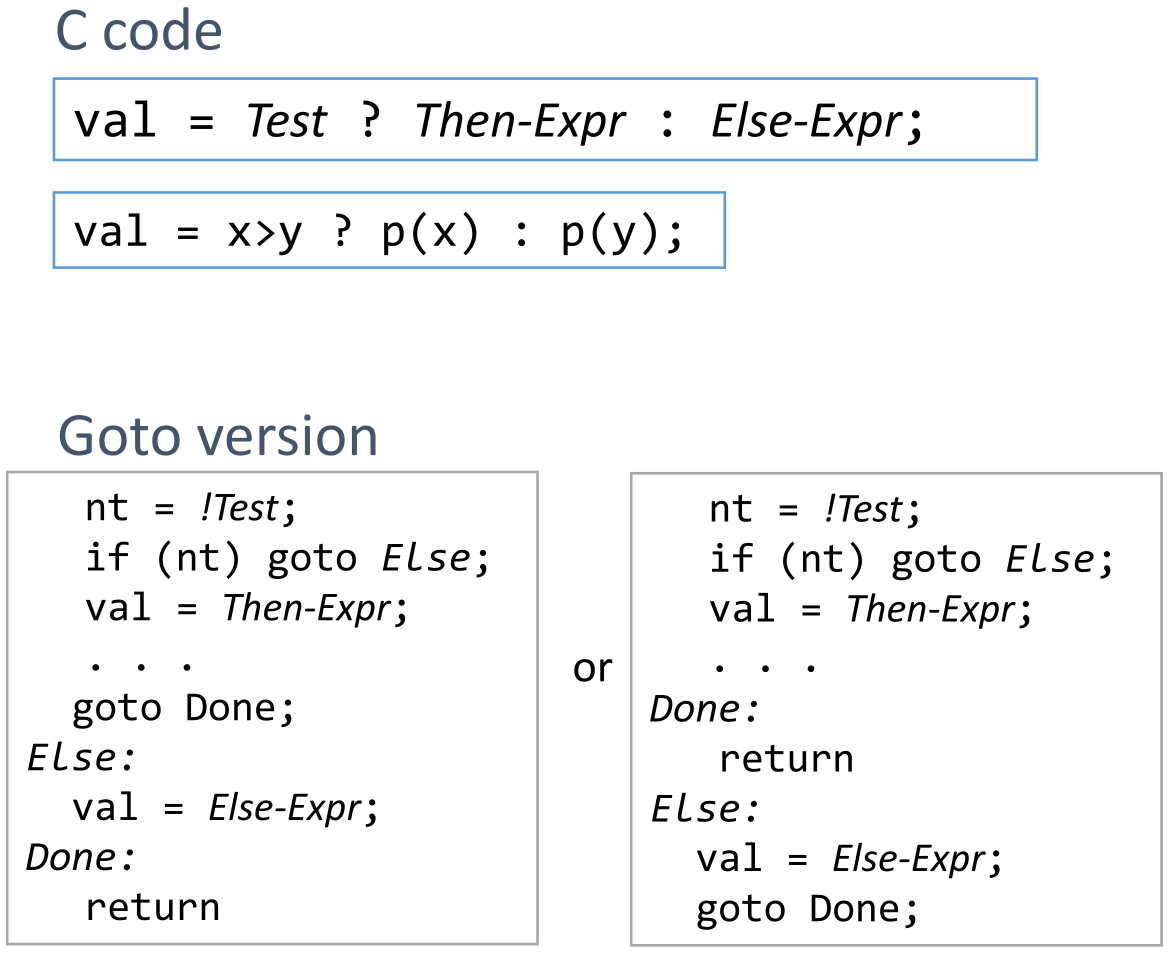
\includegraphics[width=0.5\textwidth]{10_conditional_goto.png}

Both orderings are very similar. It depends on the hardware which one is better.

Sometimes the compiler uses conditional move \code{cmovX src, dest} instead of jumps. Generally, this is more efficient event though we may have to do more work since all instructions get executed. But if the additionally work dominates or if the execution of both branches have side effects, one should not use conditional moves.

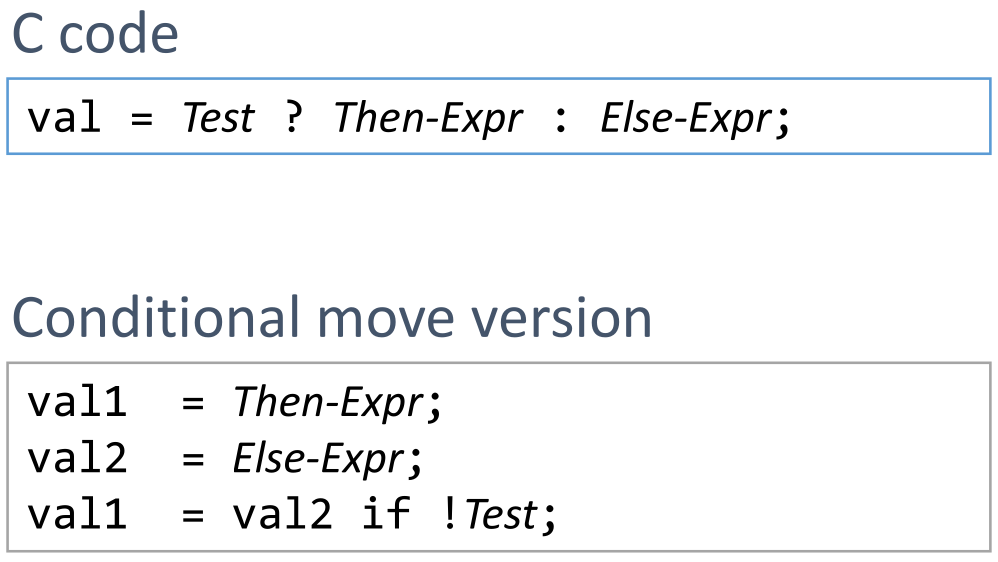
\includegraphics[width=0.5\textwidth]{10_conditional_mov.png}

\subsubsection{\code{do-while} loops}
\code{do while} are fancy conditionals with a jump. A conditional backward branch is used to continue looping as long as the condition is true.

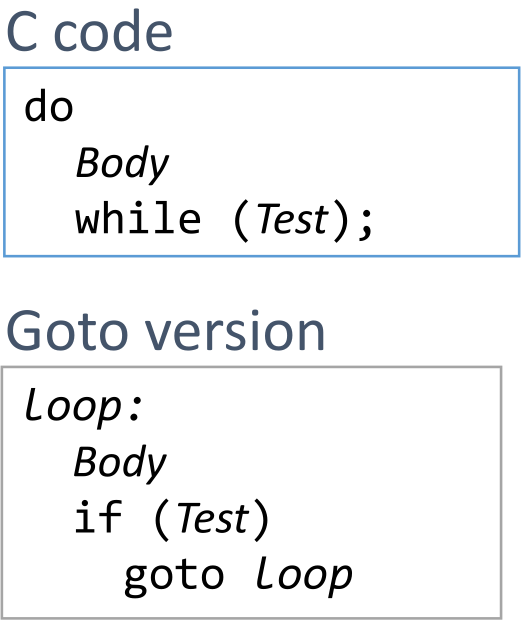
\includegraphics[width=0.5\textwidth]{10_dowhile.png}

\subsubsection{\code{while} loops}
GCC used to convert \code{while} to \code{do-whiles} with an additional conditional jump at the beginning. However, nowadays, there are separate blocks for the conditional check and the loop. At the beginning we jump to the conditional, called middle, and jump to the loop, if the condition is meat. This method is called \code{jump to middle}.

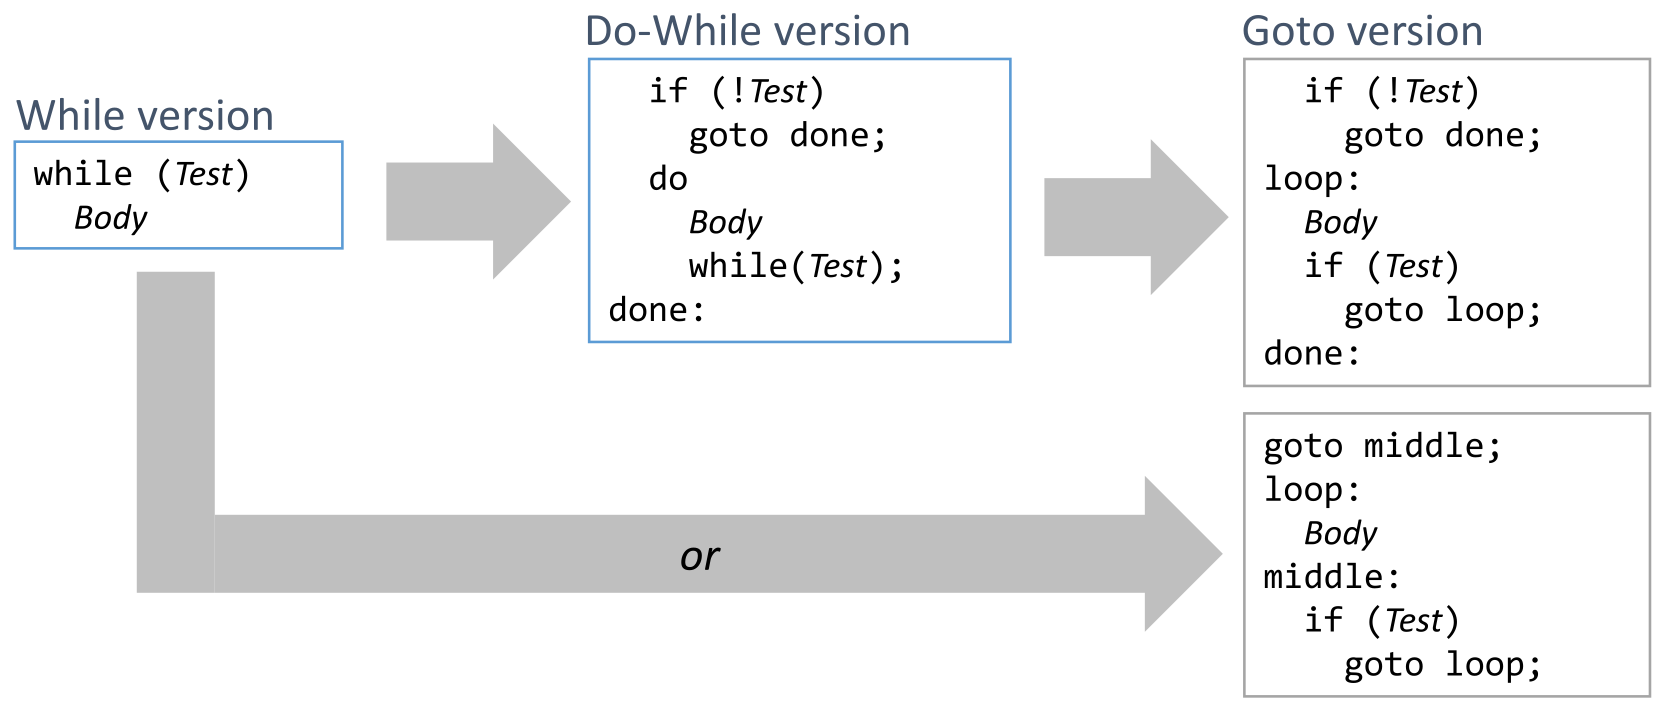
\includegraphics[width=0.8\textwidth]{10_while.png}

\subsubsection{\code{for} loops}
Are \code{while} loops with an initialisation.

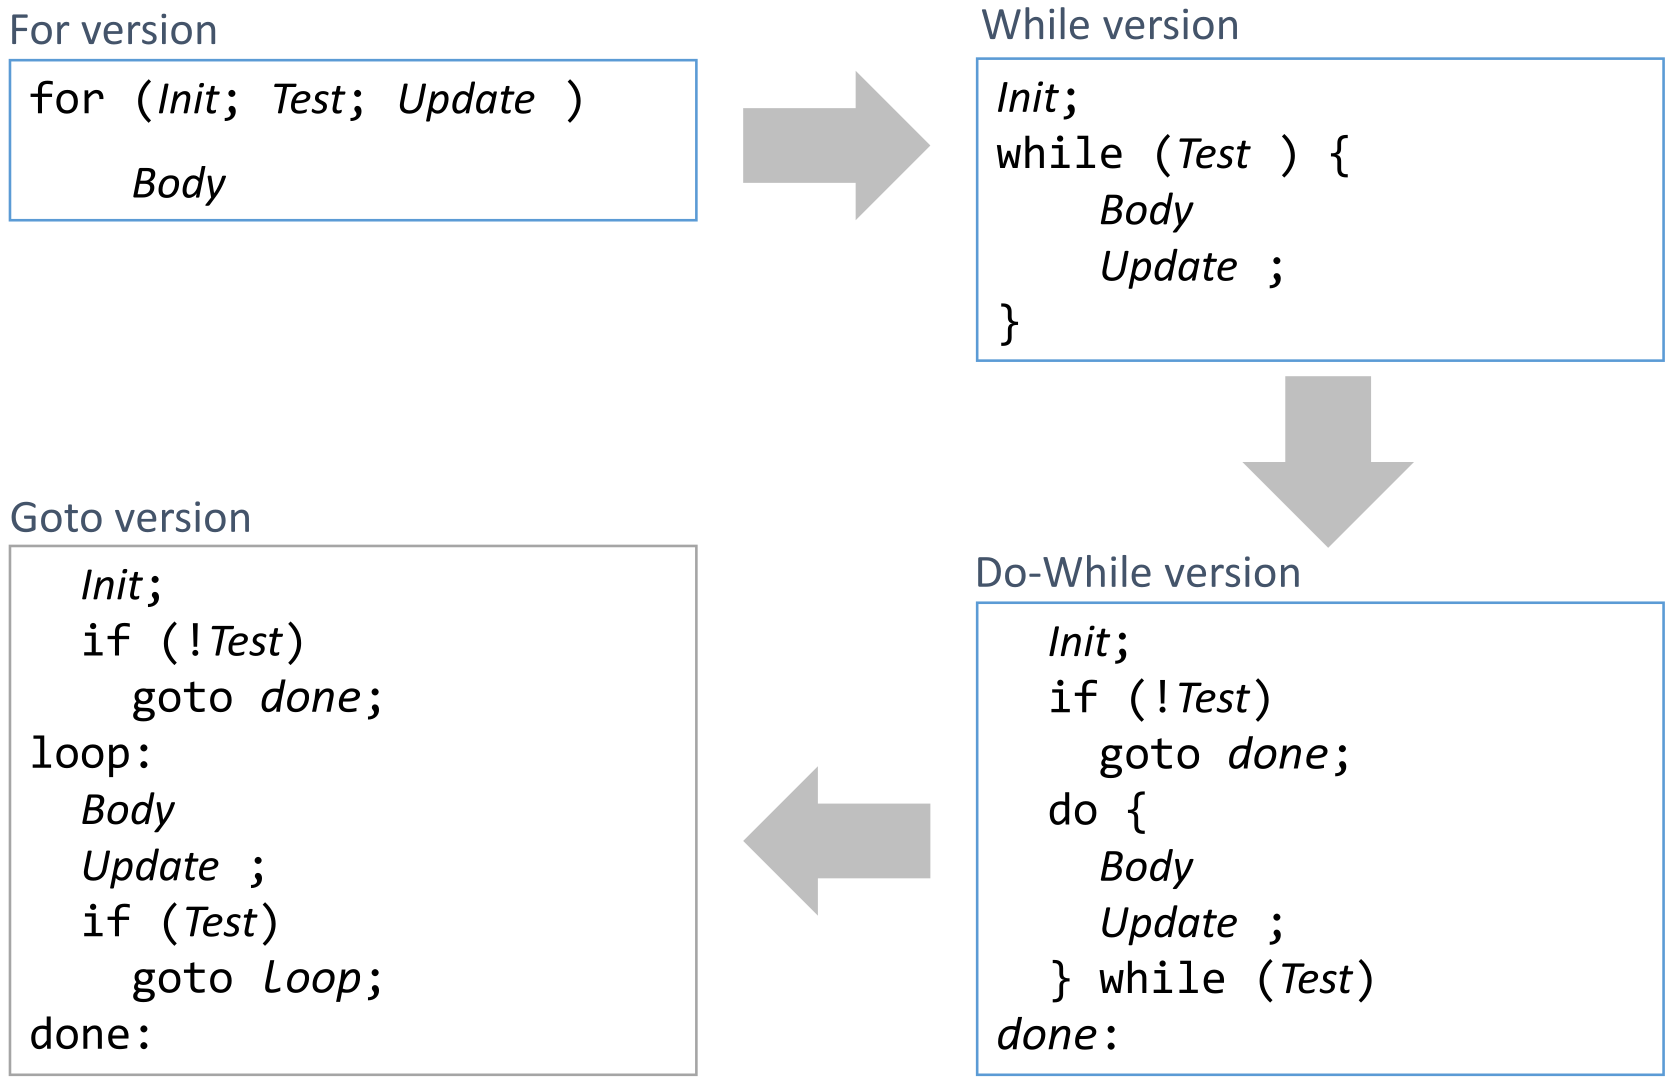
\includegraphics[width=0.8\textwidth]{10_for.png}

\subsubsection{\code{switch} statements}
The obvious way is \code{if then else}, but nobody does it. There are two kinds of statements, one where the values are compact, and switch when the values are not compact.

\subsubsection{Additional Statements:}
Anything starting with a dot in assembler is stuff not in the machine code. This is related to linking and information about what is in this file. This is handy for debugging.

\code{.text} says that code is following

\code{.global} means that the scope of the following name is global.

\code{.type} tells the type of a variable/function.

    %! TEX root = ./master.tex

\lecture{11}{Week 6}{Continue C Control Flow}

\subsubsection{\code{switch} statement}
We could implement a switch as a bunch of \code{if then else} and \code{goto} but that gets complicated with fall through and there would be very many comparisons. So compilers do not to that. Firstly, they differentiate between dense and spares \code{swtich} statements. 

\paragraph{Dense \code{switch}}
In a dense \code{switch} the values of \code{x} lie close together. For each possible case block the compiler creates an entry in the jump table. This includes cases, which land at the default. We can regard the jump table as an array which gives us for a given \code{x} the address to the jump target, which we want to execute in this case.

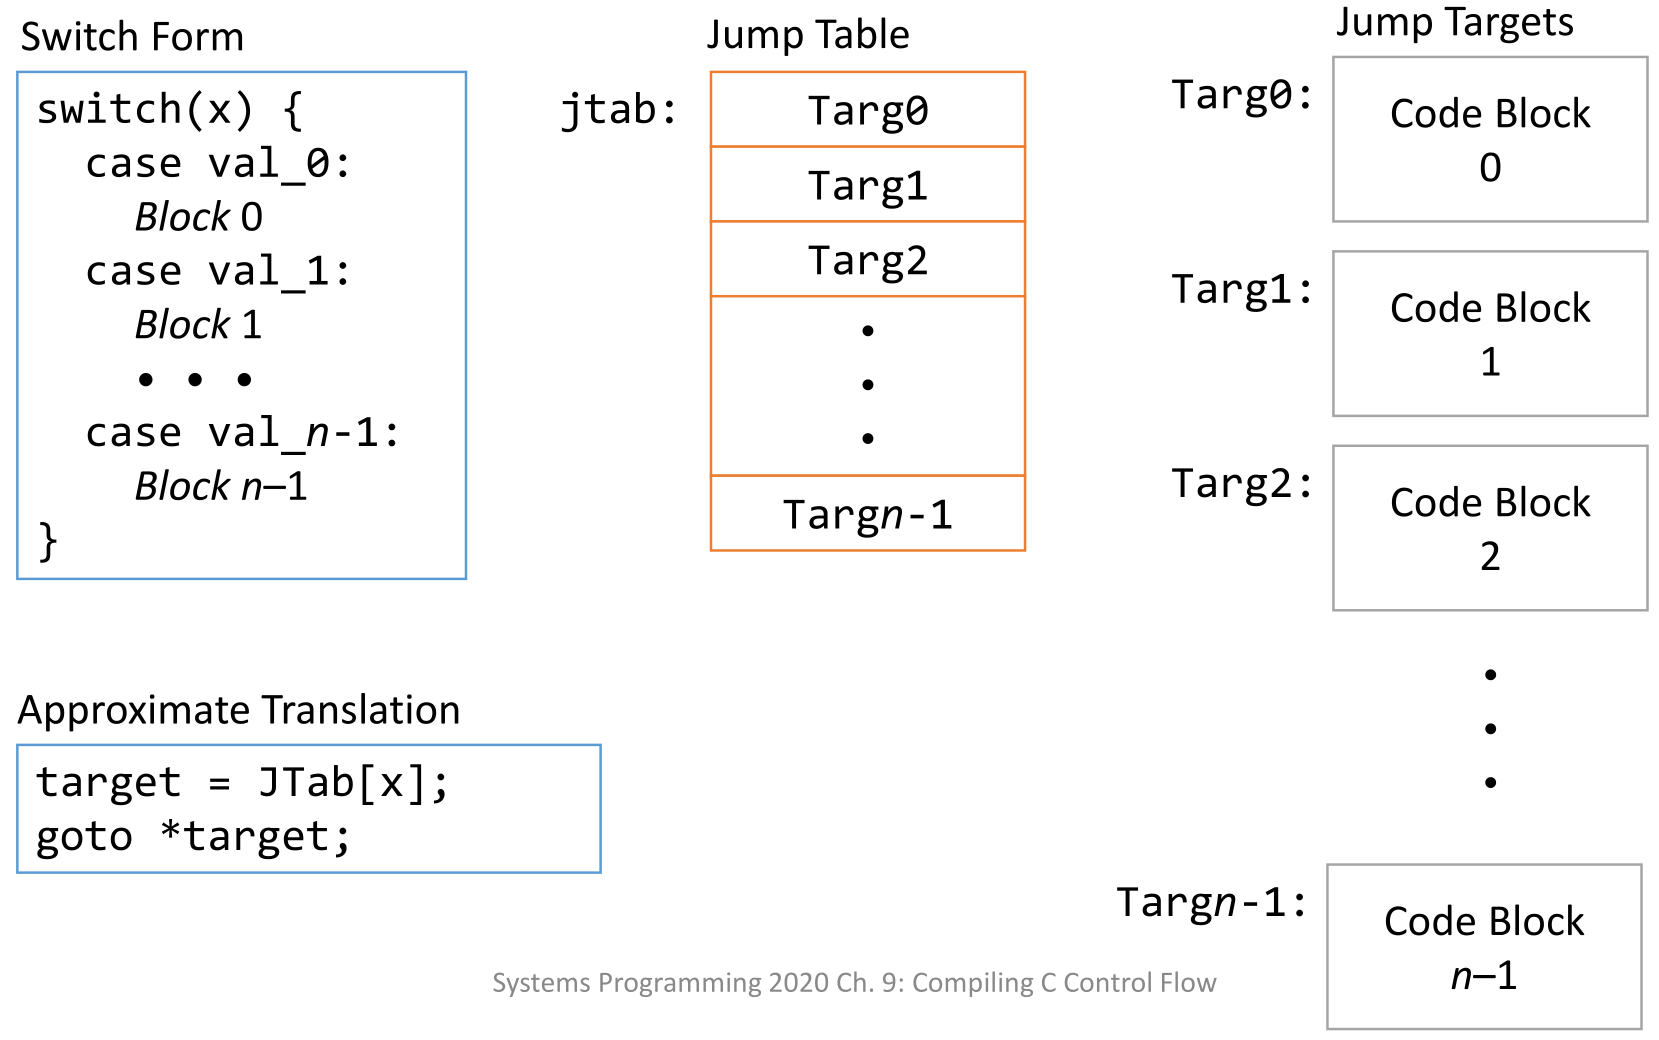
\includegraphics[width=0.8\textwidth]{11_denseswitchOverview.png}

The usage of the jump table makes the actual switch statement extremely compact. It actually only consists of a comparison, a conditional jump to the default block, and a indirect jump, via the jump table, to the designated jump target. This indirect jump could be implemented as \code{jmp *.L4(,\%rdi, 8)}, where \code{.L4} is the base address and \code{\%rdi} holds our \code{x}. We scale by $8$ since labels are $64$ bit on x86-64.

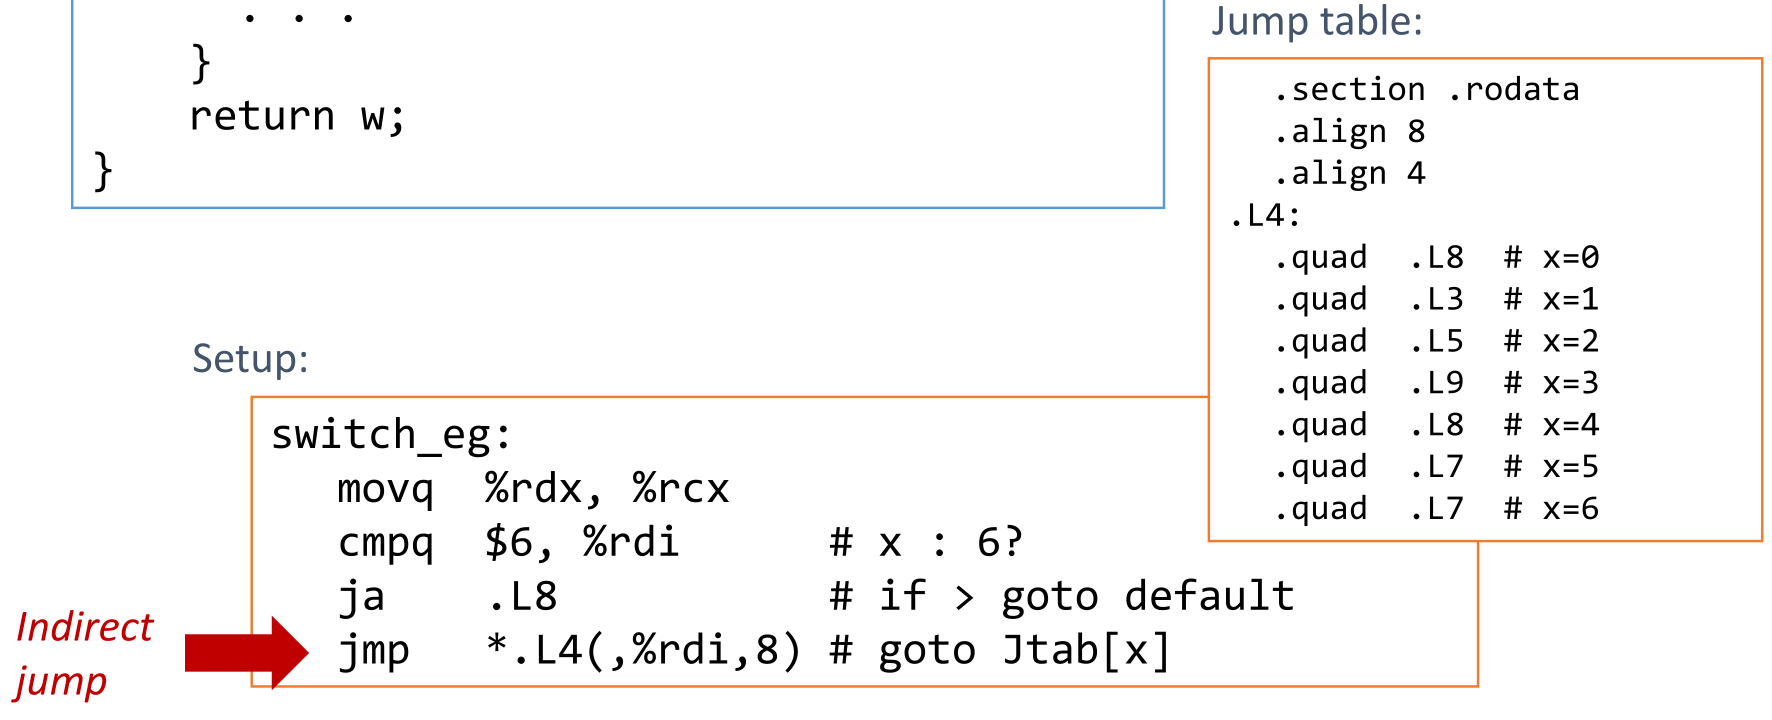
\includegraphics[width=0.8\textwidth]{11_denseswitchsetup.png}

The jump table does not seem to be in an order, that is because the compiler orders in in a way that it is most efficient.

Jump table is just data, so it does not show up in assembly or disassembled code. Nevertheless, we can inspect it using \code{gdb}.

\paragraph{Spare \code{switch}}
When there are many cases which should result in the default action, it is often too expensive to create a jump table for all these default entries. In these cases, compiler do create an binary three with three actions per node. A less than, equal and greater than. This yields logarithmic performance. In assembly this is achieved by a series of conditional jumps.

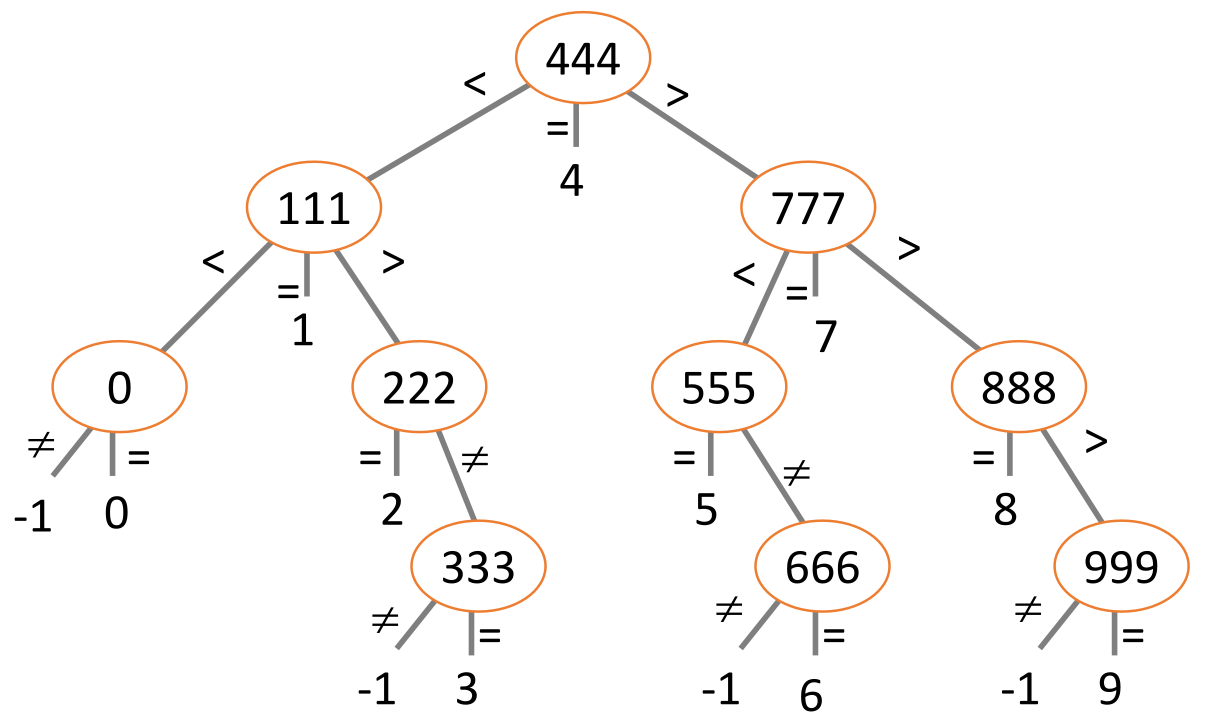
\includegraphics[width=0.8\textwidth]{11_sparseswitchtree.png}

The compile are very smart about when to use a jump table and then to rely on a search tree. We should trust the compiler in choosing the most suitable type. They may even create combinations of both types.

\subsubsection{Procedure Calls and Return}
\paragraph{Stack}
The stack is in our memory space. It starts at the top and grows downwards to lower adressess. \code{\%rsp} is the stack pointer which always points to the top (lowest address) of the stack. The stack provides the following typical CISC instructions:

\begin{description}
    \item[\code{pushl Src}:] Fetches the operand at \code{Src}, decrements the stack pointer by $4$ and writes the operand at to \code{\%rsp}.
    \item[\code{popl Dest}:] Reads the operand at the address pointed to by \code{\%rsp}, increments the stack pointer by $4$ and writes the operand to \code{Dest}.
\end{description}

These two operations are not that often used on x86-64. Even though they are very slim instructions, they are often replaced by other read and writes to relative addresses of the stack pointer.

\paragraph{Procedure Control Flow}
The stack is vital for procedure calls and returns. It is used to hold arguments, return values as well as return addresses.

In order to call a procedure, we call \code{call label}. This instruction pushed the return address on the stack and then jumps to \code{label}. The return address it vital in order to get back to the right place after the procedure has finished. In order to prevent the procedure to be called again after returning, the return address has to actually point on the address following the call instruction.

The instruction \code{ret} is called from a procedure. It pops the return address from the stack and jumps to this address.

There is no need to return after a call. This is in essence simple jump. RISC systems save the return address in a register and do not use a stack. This is called a \textit{wheeler jump}.

\paragraph{Stack Frame}
The stack frame is the current status of the stack. Generally speaking, it has the following structure.

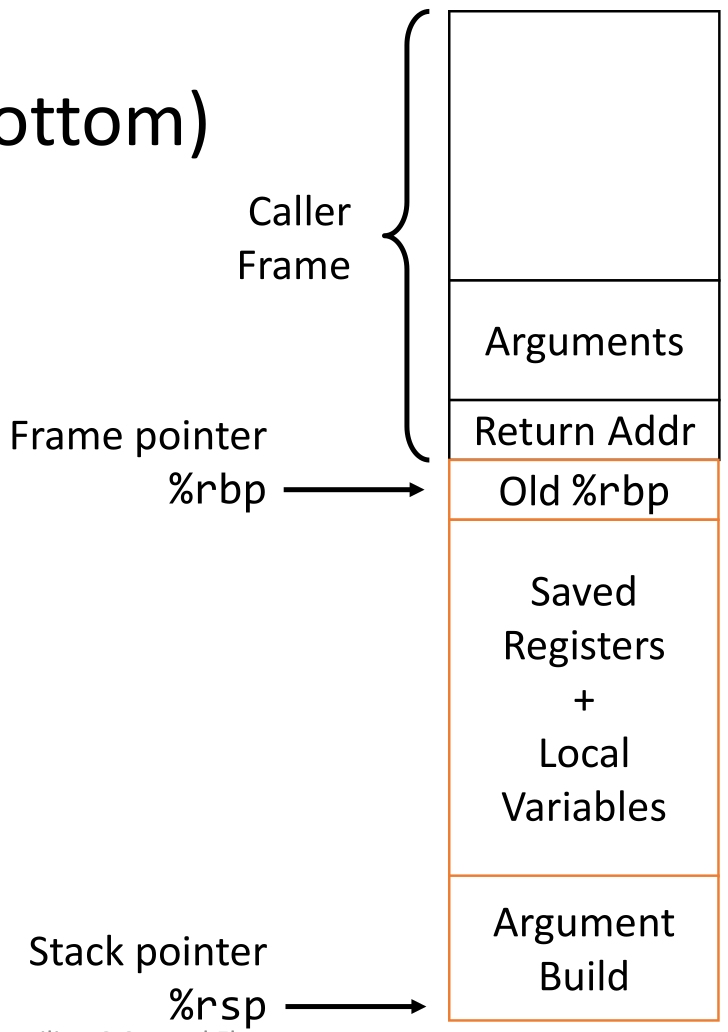
\includegraphics[width=0.4\textwidth]{11_stackframe.png}

The \textit{current stack} is the part between stack pointer and the \textit{frame pointer} \code{\%rbp}. The frame pointer points to the start of the current frame (frame contains everything related to the current procedure). At the top there are the \textit{Argument build}. It is actually not that often used nowadays. There we prepare the arguments for the function we are going to call. On top of that, there are the \textit{local variables}, which is data which we cannot keep in a register as well as the saved register content. And at the top of the current stack frame, appointed by the frame pointer, there is the \code{\%rbp} stored, of the previous frame.

Above, we find the caller's stack frame. It contains the return address and arguments passed to the call of the current procedure.

\subsubsection{Calling Convection}
There are certain conventions to which one should stick when calling procedures, and working with registers and the stack.

How do you construction procedure calls using these utilities.

\paragraph{Register Saving Conventions}
When one procedure calls another, then the one which initiates the calls ins the \textit{caller} and the one being called is the \textit{callee}. It has to be defined, which register who may change one which should stay untouched. There are the following two register types:

\begin{description}
    \item[Caller Saved:] These registers may be overwritten by the callee and therefore, it is the caller's responsibility to save them to their stack in case it needs them after the procedure returns.
    \item[Callee Saved:] These registers are long-lived and should not be overwritten by the callee. Hence, when using them they have to restore then before returning.
\end{description}

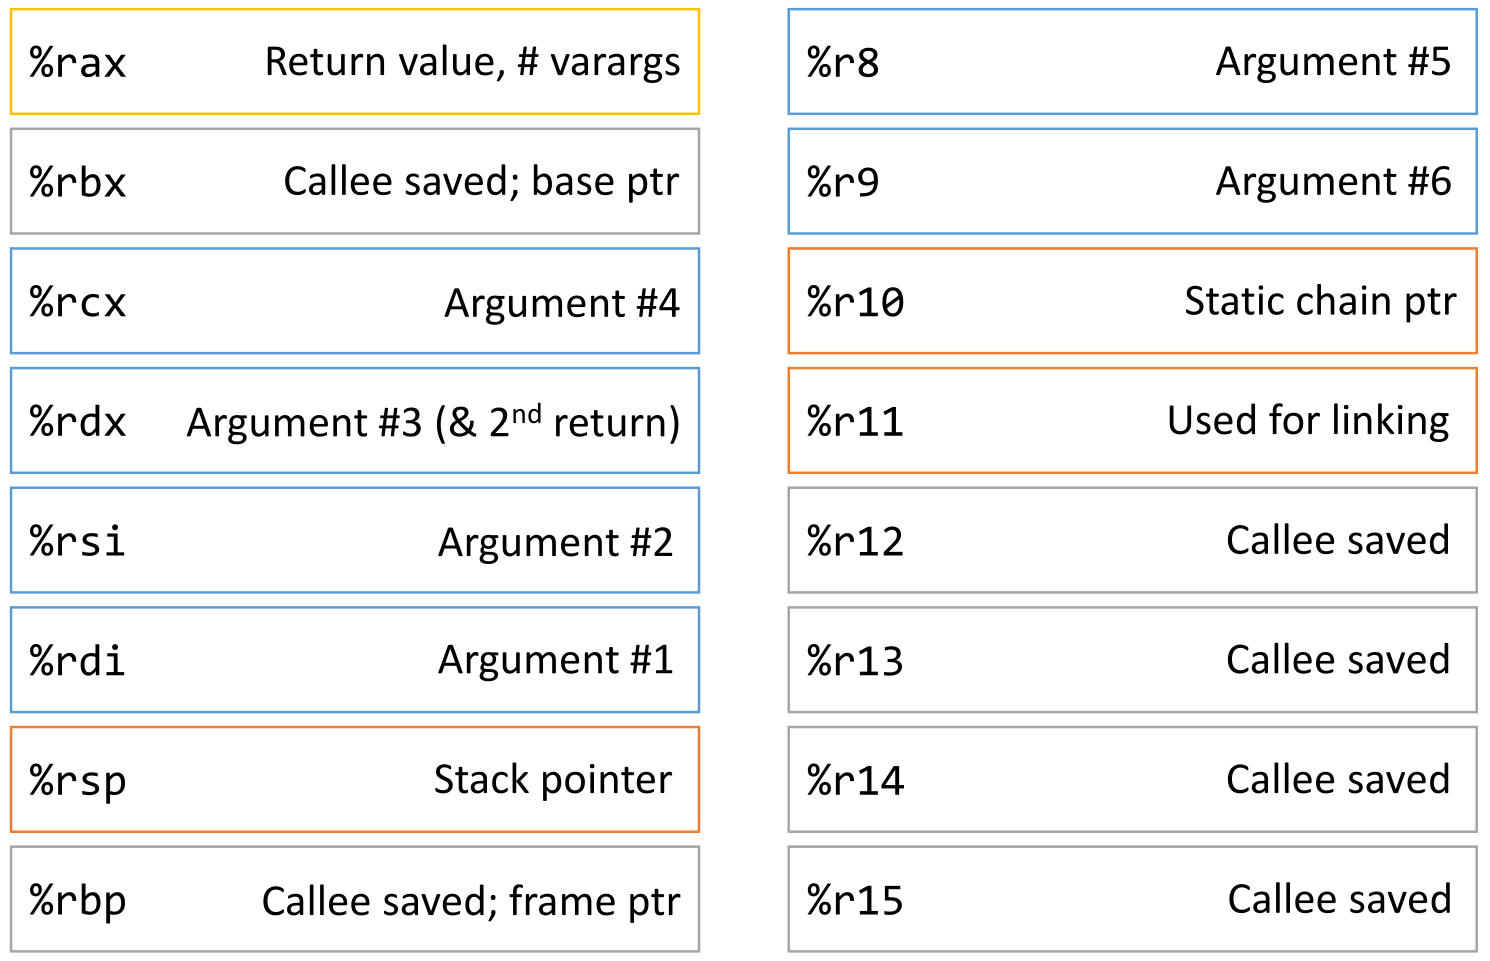
\includegraphics[width=0.8\textwidth]{11_registeroverview.png}

Arguments are passed to the callee via registers. If more than $6$ arguments are passed, the rest is passed via the stack. These registers are also used used as caller-saved and hence, can be altered by the callee.

There are two return registers. This way structs of size less than $128$ bits can be returned. If they exceed this size, they are put on the stack.

All in all, genreal purpose registers are not actually not really general purpose.

\paragraph{Working with the Stack and Stack Pointer}
All references to the stack are via the stack pointer. When the compiler adds several values to the stack (e.g. to restore callee-saved registers) it often adds then relative to the stack pointer, and decrements the stack pointer only after adding all elements. This is done for optimisation reason since the stack pointer is not decremented several times. The newly added values, which are not yet actually on the stack (stack pointer not yet updated) are in the so called \textit{red zone}.

Optimisation actions as such may break some conventions however, since it does not influence other parts, it is actually acceptable.

Other tricks are to not use the stack, to not use any callee-saved registers. In a \textit{tail call} we no not even push the current address to the stack when calling. This is useful when nested functions return (i.e. there is no need to return the inner function, just jump to the outer function which then returns). This prevents stack overflow for recursive function calls. All in all, often the stack frame is not very heavily used.

    %! TEX root = ./main.tex

\lecture{12}{Week 6}{Compiling C Data Structure}

This chapter is important because it tells us what happens in memory.

\subsubsection{Recap: Basic Data Types}
The fundamental data types on C are integers and floating-point values. They are both stored and operated on in dedicated integer respectively floating point registers. For integers, we differentiate between signed and unsigned and the interpretation depends on the used instruction.

The following table summarizes their size:

\begin{tabular}{l l l l}
    Intel & GAS & Bytes & C\\
    \hline
    byte & n & $1$ & signed/unsigned char\\
    word & w & $2$ & signed/unsigned short\\
    double word & l & $4$ & signed/unsigned int\\
    quad word & q & $8$ & signed/unsigned long int (x86-64)\\
    \hline
    single & s & $4$ & float\\
    double & l & $8$ & double\\
    extended & t & $10/12/16$ & long double\\
\end{tabular}

\textit{GAS} stands for Gnu Assembly Format.

Pointers used to be $4$ bytes long on ia32, on x86-64 they are $8$ bytes long.

\subsubsection{Arrays}
\paragraph{One-Dimensional Arrays}
One dimension arrays are blocks of homogeneous data structured contiguously in memory. The type of data it contains, determines the size of a single element. The length of the array is the size of each single block times the length of the array.

Since there is no out-of-bounds check for array, we may access random data when indexing an element which is not part of the array. When we define multiple arrays, they may be placed contiguously in memory and this way we may access the second array via the pointer of the first array. However, this is not guaranteed to works and hence, should be omitted. Compiler may arrange data in memory however they like. Compiler may also notice out-of-bound accesses and remove such instructions.

When iterating over an array and accessing its elements, compiles may eliminate loop variables and instead use pointers.

\paragraph{Nested Arrays}
Nested arrays are multidimensional arrays. Since C is row-major, row elements are stored contiguously and all the single rows itself again.

They are declared as \code{T A[R][C];} and in this example, the array would be $2$D and contains R rows and C columns. Hence, the array would be of size \code{R * C * sizeof(T)}.

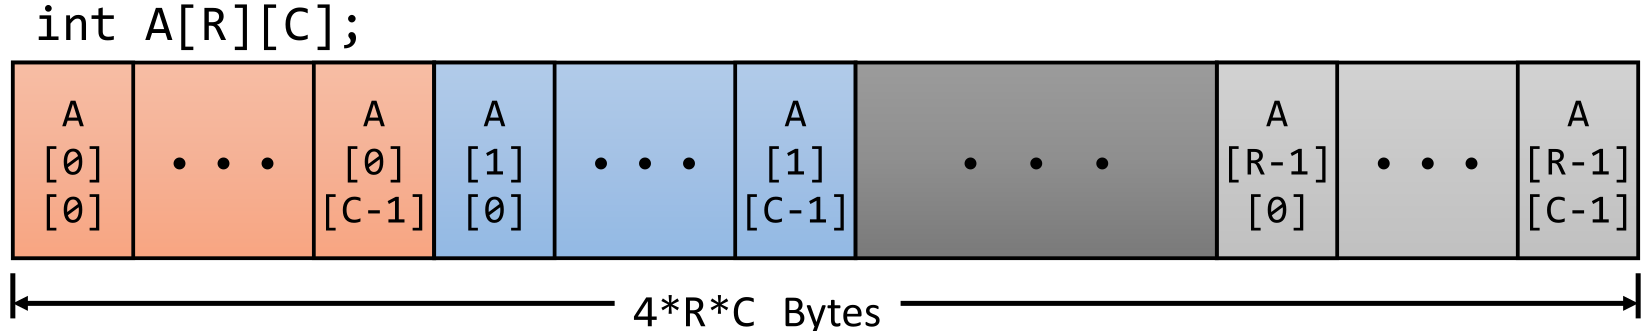
\includegraphics[width=1\textwidth]{12_nestedArrays.png}

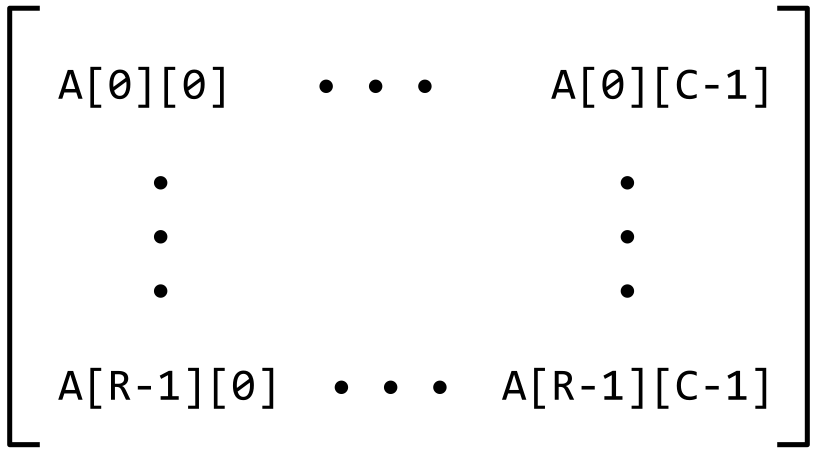
\includegraphics[width=0.8\textwidth]{12_nestedArrayStructure.png}

Since all rows are arranged contiguously, it is guaranteed that we can index into other rows. The access of any element, e.g. \code{<row>, <column>} is possible with only one memory access with the formula $base\_addr + row * column\_len * sizeof(T) + column * sizeof(T) = base\_addr + (row * column\_len + column) * sizeof(T)$.

However, there can be \textit{weird} cases where this is not guaranteed (not exam relevant...).

\paragraph{Multi Level Array}
Multi level arrays are constructed of several separate arrays. It is actually rather an array of pointers to array and it is also declared as \code{int *A[R]}. So, the rows of the array are not guaranteed to be placed contiguously in memory and therefore, one cannot access any element of the array by adding an offset to the base pointer. But instead, we have to first access the \textit{pointer array}, and then access the desired element. This requires two memory accesses compared to only one for nested arrays. For arrays of higher dimension, even more memory accesses are required.

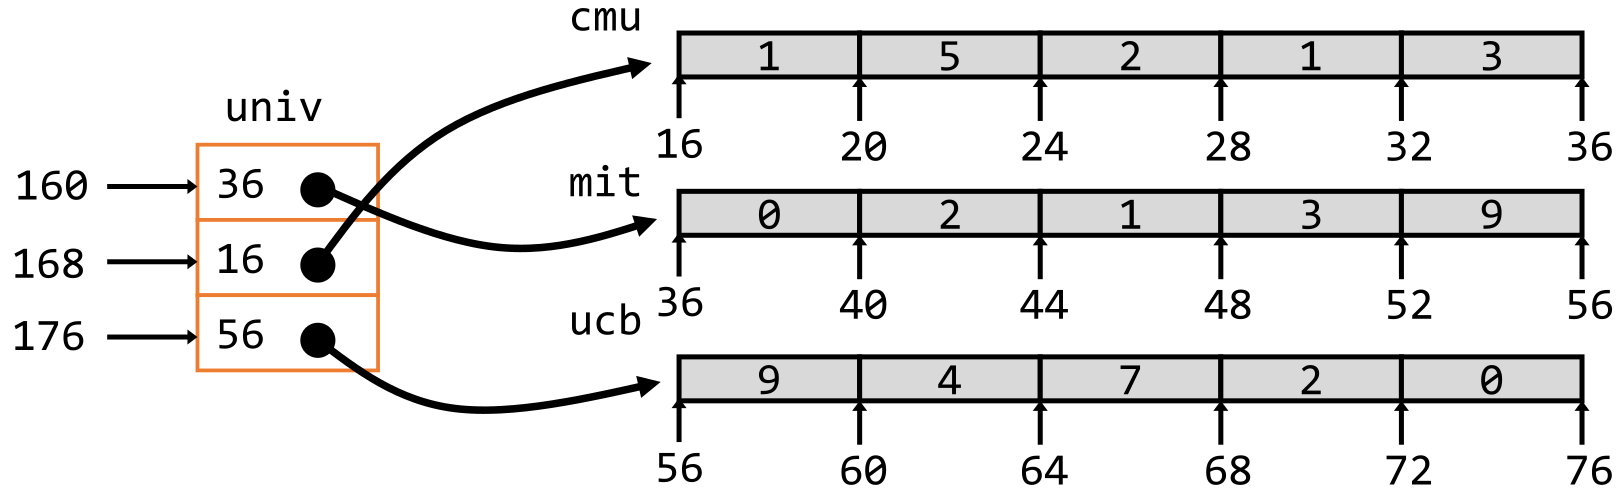
\includegraphics[width=1\textwidth]{12_multilevelarrayoverview.png}

\paragraph{Arrays for Matrix Multiplication}
Compilers are good at doubly subscripted array accesses. However, in order to implement represent an matrix with nested arrays, its size needs to be known at compile time. When we want it more dynamically, we may implemented the \textit{nested array structure ourself} by heaving a block of memory and do all index computation by ourself. Since we need to do many multiplications and access of single elements are therefore rather costly, this is not very performant. Nevertheless, compiler are actually quite good ad improving this solution since there are many regular patters for e.g. a matrix multiplication.

\subsubsection{Structures}
Stucts are a contiguously-allocated region of memory. The values are ordered contiguously in the same order as their are defined. Since they are arrange contiguously, we can theoretically access a subsequent element via the address of a previous element.

\paragraph{Alignment}
For performance reasons, data is always aligned in memory. If it ways not, maybe multiple memory accesses may be required to read or write instead of just one, because memory is accessed in junks of $4$ or $8$ bytes (system dependant).

For x86-64 we have to following alignment cases:
\begin{description}
    \item[1 byte:] char
    \item[2 bytes:] short
        \begin{itemize}
            \item lowest $1$ bit of address must be $0_2$
        \end{itemize}
    \item[4 bytes:] int, float
        \begin{itemize}
            \item lowest $2$ bits of address must be $00_2$
        \end{itemize}
    \item[8 bytes:] double, char, *
        \begin{itemize}
            \item lowest $3$ bits of address must be $000_2$
        \end{itemize}
    \item[16 bytes:] long double
        \begin{itemize}
            \item lowest $3$ bits of address must be $000_2$ (treated equivalently to $8$ byte aligned types)
        \end{itemize}
\end{description}

In short this means that if a primitive data type requires $K$ bytes, it is always aligned on a multiple of $K$.

In order that the data fields in the strut are aligned, the compiler may add padding between fields. Therefore, it is also not guaranteed that we can access a subsequent field by simple adding some padding. The placement of the struct itself is determined by the sizes of its fields. If $K$ is the alignment of the largest field, then the struct is aligned at a multiple of $K$.

It may be optimal to define files of larger types first, but since the whole struct must be aligned in a multiple of the size of the largest fields, in practice there is not much gain.

\paragraph{Arrays of Structures}
Stucts in arrays have to follow the alignment requirements too. This may lead to lots of unused padding space.

\subsubsection{Union}
The size of a union is simply the size of the largest field. The space for the fields is \textit{overlayed}.

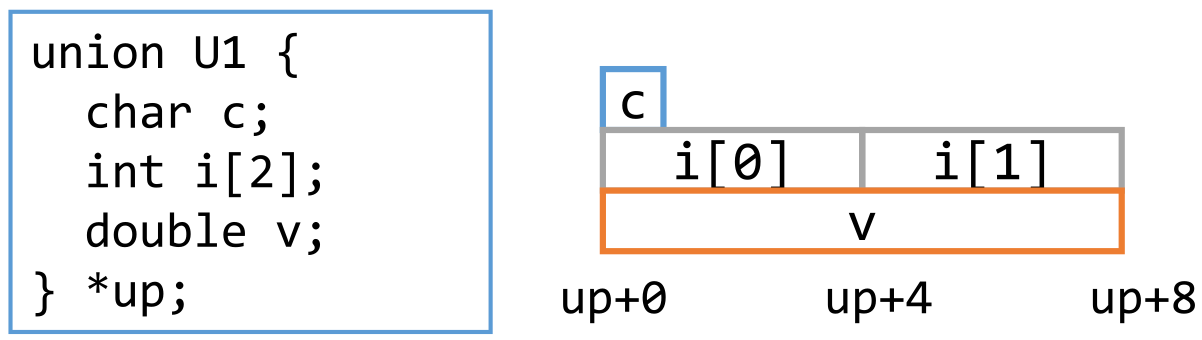
\includegraphics[width=0.8\textwidth]{12_union.png}

    %! TEX root = ./main.tex

\lecture{13}{Week 7}{Linking}
When a project in split into multiple files \code{.c}, they are compiled independently into object files \code{.o}. The linker is then responsible for combining all object files into the final executable. The Unix linker is called \code{ld} but since gcc is actually a wrapper of many programs, it does also the linking part.

When we compile a file using ggc, the \code{-g} flag makes sure that debugging information remains in the executable.

\subsubsection{Why Linkers}
\begin{description}
    \item[Modularity:] Linkers allow to break a project into many small pieces on which one can work independently. Furthermore, linkers allow to build libraries.
    \item[Efficientcy:] Linkers allow to write efficient code in two ways:
        \begin{itemize}
            \item Compiling takes time. Then only one file changes, it would be wasteful to recompile also the unchanged files. 
            \item We can put function which may be reused in a dedicated file. This allow for simple reuse as well as lower memory usage when loading this function, since the file only contains code we actually need.
        \end{itemize}
\end{description}
\paragraph{Modularity}

\subsubsection{What does a Linker do?}
Linking is a two-step process:
\begin{description}
    \item[1. Symbol Resolution:] Programs define and reference symbols. Symbols are function names and variables. The symbols definitions get stored into the symbol table by the compiler. This is an array of stucts where each entry includes symbol name, type, size and location. The linker then associates each symbol reference with exactly one symbol definition.
    \item[2. Reallocation:] The linker merges separate code and data section into a single section. This requires the reallocation of the symbols from their relative location in the \code{.o} files to their final absolute memory location in the executable.
\end{description}

\subsubsection{Object Files}
There exist three different kinds of object files (modules):
\paragraph{Relocatable Object Files}
They have the extension \code{.o} and each single file is the product of a compiled source file. They contain code and data which is in a format, such that it can be combined with other relocatable object files to form an executable. 

\paragraph{Executable Object Files}
They contain code and data which can be directly copied to memory and executed.

\paragraph{Shared Object File}
They have the \code{.so} extension. These are special object files which have the property, that they can be loaded and linked dynamically at runtime, into memory.

\paragraph{Executable and Linkable Format (ELF)}
All mentioned object files types share the same format. The ELF is the standard finery format for object files and the generic name for such object files is ELF binary.

A section referees to bits of a file where segments referees to bits in memory.

The general format is as follows:
\begin{description}
    \item[Elf Header:] Tells that this file is in the ELF format as well as provides information about endianess, word size, machine type, file type etc.
    \item[Segment Header Table:] Contains information about the page size, virtual address memory segments (where is stack, heap etc), segment size.
    \item[.text section:] Machine code given by the compiler.
    \item[.rodata section:] Read-only data like the jump-table.
    \item[.data section:] Initialized global variables. The last segment tells where the .bss section starts.
    \item[.bss section:] Uninitialized global variables. Since they have no value, it is normally smaller than the data segment. Called \textit{Block Started by Symbol} or \textit{Better Save Space}.
    \item[.symtab section:] Symbol table and the names of procedures and static variables.
    \item[.rel.text section:] Reallocation information for .text section (addresses of instruction which need to be modified as well as instruction for modifying).
    \item[.rel.data section:] Reallocation information for .data section (addresses of pointer data which need to be modified).
    \item[.debug section:] Information fo symbolic debugging with \code{gcc -g}.
    \item[Section Header Table:] Offset and sized of each section.
\end{description}

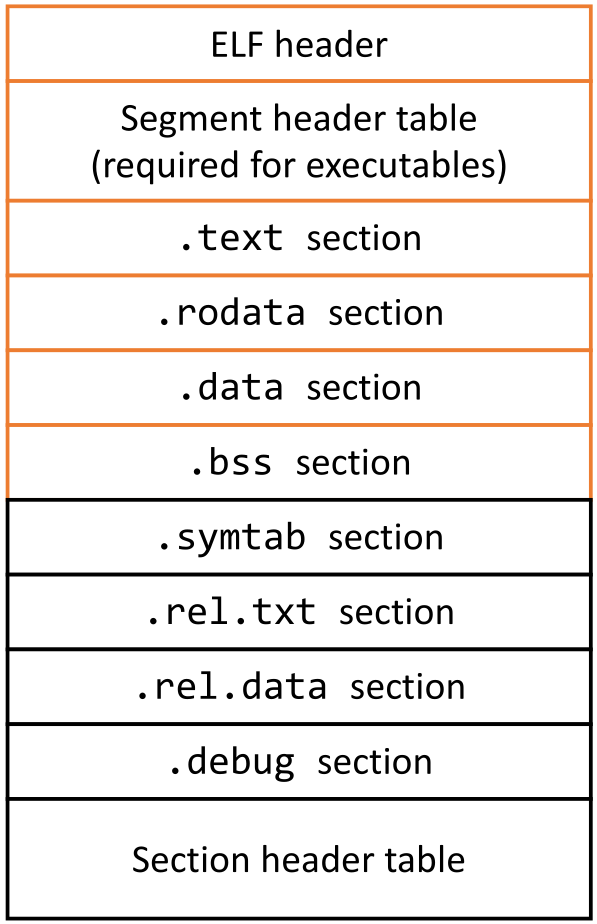
\includegraphics[width=0.8\textwidth]{13_elfformat.png}

\subsubsection{Linker Symbols}
There are three types of symbols:
\paragraph{Global Symbols}
Symbols which are defined as globals in a certain module.

\paragraph{External Symbols}
Symbols which are referenced in a certain module, but defined in another module. One can prepend external symbols by \code{extern}. This is not required, nevertheless, one should always do it for good practice.

\paragraph{Local Symbols}
Symbols which are defined and referenced only in a certain module. However, they are \textbf{not} local program variables. Linkers are not aware of any local program variables.

\paragraph{Example Linker}
Given the following code, we can find the symbols and their type:

\includegraphics[width=0.8\textwidth]{13_linkersymbols.png}

The linker combines them as follows into an executable. The system code and data is stuff the compiler sees but we do not.

\includegraphics[width=0.8\textwidth]{13_realocatingCodeData.png}

In the disassembled .tex section of main.o we see, that the compiler does not know where swap is. Instead, it inserted an entry into the symbol table (the string in read). String tells that at address $a$ there are $4$ bytes which need to be filled with the address of the function called \code{swap}. The \code{R\_X86\_64\_PC32} means it is a reallocation entry for a x86-32 processor which used pc relative $32$ addressing. This information allows the linker to fill in the right address.

\includegraphics[width=0.8\textwidth]{13_ex_maintext.png}

The disassembled .data section we can see the global two integer.

\includegraphics[width=0.8\textwidth]{13_ex_maindata.png}

The first movq instruction has again two $4$ byte long addresses of zero. The first address is again a PC relative $32$ offset reallocation instruction. It is the unallocated \code{bufp1} symbol and hence, it is referred to as \code{.bss-0x8}. The second address is again a reallocation entry but it is a $32$ bit scalar value, which is referred too as \code{buf+0x4}.

\includegraphics[width=0.8\textwidth]{13_ex_swaptext.png}

In the data section we find the \code{buf}. In the bss section we find the \code{bufp1} symbol. it has $8$ bytes, but they are actually not in the file, it is just recorded that they should be there.

\includegraphics[width=0.8\textwidth]{13_ex_swapdatabss.png}

The linker takes the previously discussed files, and puts them into a single executable. The .text section looks as follows. The file looks very familiar, but the missing addresses were filled in (the linker reallocated the addresses). 

\includegraphics[width=0.8\textwidth]{13_ex_exectext.png}

And the .data and .bss. We notice that all addresses are only $8$ bytes long. The reason is in order to save space. The compiler uses relative addresses and the linker figures out what this address is.

\includegraphics[width=0.8\textwidth]{13_ex_exec_databss.png}

\paragraph{Strong and Weak Symbols}
\begin{description}
    \item[Strong:] Procedures and initialized globals
    \item[Weak:] Uninitialized globals
\end{description}

\paragraph{Linker's Symbol Rules}
Then multiple symbols with the same name are given the linker proceeds as follows:

\begin{enumerate}
    \item Multiple string symbols are not allowed. This leads to a linker error.
    \item When given a strong and multiple weak symbols, the liner always chooses string symbol. So, references to the weak symbol resolve to the strong one.
    \item When given multiple weak symbols, the linker picks one arbitrary. This can lead to weird problems. E.g. when there are two structs with the same name and same size, but different fields (one has two ints, the other one double), the linker may select one at random and when writing to e.g. the address of the first int, we may be dealing with a double of the size of both ints. This problem may also arise when we combine code which was compiled by different compiler which have different alignment rules.
\end{enumerate}

\paragraph{Some Puzzles}
Some Linking Puzzles:

\includegraphics[width=0.8\textwidth]{13_linkerpuzzles.png}

\paragraph{Global Variables}
Globals can cause many issues. Besides the already disused ones, it may also quickly happen that different programs declare globals with the same name. Good practice is to avoid them when possible. If not, one should at least initialized them. An when using an external global, one should always prepend it by \code{extern}.

\subsubsection{Static Libraries}
We may want to package commonly used functions into a library. Trivial ways to accomplish that is by putting all function into a single source file or by putting each function into a separate file. Both methods have some downsides. While the first methods is very space and time inefficient, the second methods puts a burden on the programmer to link the appropriate binaries into their programs.

Static libraries solve this problem. They have the extension \code{.a} and the concatenate related relocatable object files into a single archive file. The linker tries to resolve unresolved external references by looking for that symbol in one or multiple archived. On success, the linker links the object file into the executable.

The following diagram shows the usage of static libraries:

\includegraphics[width=0.8\textwidth]{13_staticlibrarydiagram.png}

\paragraph{Build Archives}
The archiver \code{ar} is used to create such archives:

\includegraphics[width=1\textwidth]{13_staticlibrary.png}

The archiver allows incremental updates. This means that when a function changes, only the source of that file is recompilation and the .o file is replaced in the archive.

How does the linker know where these archives are? There are certain defaults directories. To include certain libraries, it is also possible to load it with \code{gcc -lm} where \code{m} is the name of the library (in this case libm (the math library)).

\paragraph{How Linker Resolve External References}
The linker scans the .o files and .a archives in the ordre they were provided to the command. During the scan, it weeks a list of currently unresolved reference. Always when a new archive .a or object .o file is encountered, it tries resolve unresolved reference and updates the unresolved references list. If at the end of this process there are unresolved reference, this leads to an error.

The main problem is, that the linker does only one pass of this algorithm. Since files are scanned in the order they are provided, one should put libraries at the end of the command. E.g. \code{gcc -L. libtest.o -lmine} instead of \code{gcc -L. -lmine libtest.o}.

\paragraph{Loading an Executable Object File}
When loading an executable, different sections are put into corresponding segments in memory. It used to be the way, the executables would be put directly into memory in reversed order.

\includegraphics[width=0.8\textwidth]{13_loadingexecutables.png}

\subsubsection{Shared Libraries}
Since when using static libraries, all code is copied into the executable, one has to recompile the program, when the library is updated. Further, the code is always duplicated. Therefore, static libraries are only actually used during the building process and shared libraries in production.

Shared libraries provide object files containing code and data which get linked into a program dynamically during load-time or run-time.

Shared libraries are also called dynamic link libraries (DLLs) and they can be shared between multiple processes.

\paragraph{Load-Time Linking} is automatically handled by the dynamic linker \code{ld-linux.so}. The following graphic depicts the procedure:

\includegraphics[width=0.8\textwidth]{13_dynamicLinking.png}

\paragraph{Run-Time Linking} is done by calls to \code{dlopen()} interface.

\includegraphics[width=0.8\textwidth]{13_runtimeI.png}

\includegraphics[width=0.8\textwidth]{13_runtimeII.png}





main+addr is used then the location of the function is unknown. The linker is responsible to fill in the missing address at address $a$. The red string is stored in the symbol table. 

.bss-0x8 stands for the rip we do not know. The buf+0x4 is a scalar value and is the 

compiling p2 alone, we get something in the .bss called foo
compiling p1 alone, we get something in the .data called foo

if the two files are linked together, we only get one foo, and this is the p1 because the linkers sees assumes that the foos are equivalent

    %! TEX root=./master.tex

\lecture{14}{Week 7}{Code Vulnerabilities}

\subsubsection{Worms And Viruses}
Both viruses and worms are designed to spread among computers, network and drives. Though they are fundamentally different:

\begin{description}
    \item[Worm:] is a program than runs by itself and which is capable to propagate a fully working version of itself to other computers.
    \item[Virus:] is code which adds itself to other programs ant it cannot run without its \textit{host} program.
\end{description}

In the early days of computers, worms were actually used in distributes systems for e.g. update purpose. The first \textit{malicious} worms was written in 1988 by Robert Morris and was designed to count the number of hosts on a network. 

\subsubsection{Stack Overflow Bugs}
This is one of the simplest code vulnerability bugs one can exploit.

\code{gets} is a C functions which ready input till it receives an \textit{end-of-file} character and stores them in an array designated by a pointer. The problem with this early implementation was, that there is no way to specify the maximal number of characters to read.

\includegraphics[width=0.8\textwidth]{14_gets.png}

The previous code works perfectly for inputs of length $3$ (the $4$-th byte is required for the end character) or maybe even for a few more bytes, but when we input a large amount of characters we get a segmentation fault. 

A stack frame of a certain size gets initialized and the buf variable is stored within in.

\includegraphics[width=0.8\textwidth]{14_getsStack.png}

As long as we only overwrite data in the stack frame, this may not cause direct problems, when when the return address gets overwritten, we will receive a segmentation fault.

\includegraphics[width=0.8\textwidth]{14_getssegmentation.png}

Instead of simply crashing the program, we may make malicious use of this vulnerability. My overwriting the return address of another stack frame and make it point to some exploit code which we have pushed to the stack via gets.

\includegraphics[width=0.8\textwidth]{14_maliciousoverflow.png}

There used to be a server called \code{fingered} which used \code{gets}. Instead of calling it like \code{finger username@addres}, one could execute something like \code{finger "exploit code padding new-return-address"} which then gets executed on the root shell.

\paragraph{Prevent Stack Overflow Issues}
There are several ways to prevent these issues. One should for example always use the more modern and robust functions. I.e. use \code{fgets} instead of \code{gets}, \code{strncpy} instead of \code{strcpy} and \code{fgets} instead of \code{scanf} for reading strings (or use \code{\%ns} instead if \code{\%s}).

Further, one should also always take care when defining these limits. It is actually really hard to get them right. It can easily happen that the end character is forgotten.

Compilers do have a notion about libraries (which is not only something positive...) and may detect such issues. For experimentation purpose we can disable this feature using the flags \code{-D\_FORTIFY\_SOURCE=0} and \code{-fno-stack-protector}.

In order to make it more difficult for a attacker to guess the right address, stack offsets are initialized at random. Furthermore, some CPUs can make certain parts of the memory read- or write only. Or they can make the stack non-executable, meaning that no code on the stack can be executed. However, we can still use e.g. the heap for exploit code and therefore, this is not really a fix.

All in all, even though this problem is mostly  fixed, it still pops up from time to time. 

\subsection*{Floaging Point}
\subsubsection{Representing Floating-Point Numbers}
Fractional binary numbers can be very intuitively represented as $\sum_{k=-j}^{i} b_k \cdot 2^k$. All bits to the right of some \textit{binary point} represent fractions of powers of $2$.

\includegraphics[width=0.8\textwidth]{14_fractionalrepresentation.png}

As we are used to from integers, a right shift represents a division of $2$ and a left shift a multiplication by $2$. 

The problem with this representation is that, we can only exactly represent numbers which are of the form $\frac{x}{2^k}$. In order to represent any number exactly we would need infinitely many decimal points.

\paragraph{IEEE Floating Point}
In the early days, there was no standard on how to represent binary numbers, and all CPU manufactures implemented their own format. In 1985 the first standard for floating point arithmetic was introduced. It was supported by all major CPUs.

Floating point numbers are represented in the form $(-1)^S \cdot M \cdot 2^E$.
\begin{description}
    \item[S:] sign bit determines whether the number is positive or negative.
    \item[M:] is the significant and it is a fractional value in the range $)1.0, 2.0)$.
    \item[E:] exponent weight.
\end{description}

The $M$ and $E$ are not directly stored as twos complement, but encoded in a specific was. This allows the format to represent a much wider range. The encoding is as follows:
\begin{description}
    \item[s:] directly represents the $S$ and is the MSB of the encoding.
    \item[exp:] is the encoding of $E$
    \item[frac:] is the encoding of $M$
\end{description}

\includegraphics[width=0.8\textwidth]{14_encoding.png}

The length of the exp and frac section is determined by the used Standard.

\includegraphics[width=0.8\textwidth]{14_percisionstandardtable.png}

There used to be the two single and double precision standards. Over time the total length got bigger. But only recently a few other, much shorter non-standards, but widely used ones, were introduced. They are used mainly for machine learning. One found out that it is worth trading precision for efficiently.

\paragraph{Floating Point in C}
In C99, float (single precision) and double (double precision) are guaranteed to have a certain size independent of the machine. Other types vary in length.

When casting one type to another, the bit representation changes. This is very different from the signed/unsigned integer representation, where only the interpretation changed.
\begin{description}
    \item[double/float $\to$ int:] truncates fractional parts which is equivalent to a rounding towards zero. The behaviour is undefined when out of range.
    \item[int $\to$ double:] As long as the int has less that $\le 53$ bit word size, the conversation is exact.
    \item[int $\to$ float:] Will round according to the rounding mode.
\end{description}

Floating point numbers are einher normalized, or denormalized:
\paragraph{Normalized Values}

\begin{itemize}
    \item This are numbers, where $exp \neq 000 \dots 0$ and exp $\neq 111 \dots 1$.
    \item E is encoded as $E = Exp - Bias$ 
        \begin{description}
            \item[Exp:] is the unsigned value of exp
            \item[Bias:] is equal $2^{e-1} - 1$, where $e$ is the number of exponent bits.
                \begin{description}
                    \item[Singe Percision:] $Bias = 127, Exp \in [1, 254], E \in [-126, 127]$
                    \item[Double Perc.:] $Bias = 1023, Exp \in [1, 2046], E \in [-1022, 1023]$
                \end{description}
        \end{description}
    \item M is equal to $1.xxx \dots x_2$ where $xxx \dots x$ are the bits of frac.
        \begin{itemize}
            \item Minimum when $000 \dots 0 \implies M = 1.0$
            \item Maximum when $111 \dots 1 \implies M = 2.0 - \epsilon$
        \end{itemize}
\end{itemize}

\paragraph{Example}
Normalized encoding of $15213.0$:

\includegraphics[width=0.8\textwidth]{14_normalizedexample.png}

\paragraph{Denormalized Values}
\begin{itemize}
    \item These are numbers, where $exp = 000 \dots 0$.
    \item E is encoded as $E= -Bias + 1$
        \begin{description}
            \item[Bias:] is equal $2^{e-1} - 1$, where $e$ is the number of exponent bits.
                \begin{description}
                    \item[Singe Percision:] $Bias = 127, Exp \in [1, 254], E \in [-126, 127]$
                    \item[Double Perc.:] $Bias = 1023, Exp \in [1, 2046], E \in [-1022, 1023]$
                \end{description}
        \end{description}
    \item M is equal to $0.xxx \dots x_2$ where $xxx \dots x$ are the bits of frac.
\end{itemize}

When $exp = 000 \dots 0$ and one if $frac = 000 \dots 0$, the number is zero. Depending on $s$, we have actually $-0$ and $+0$. This is actually useful to distinguish between convergence from below and from above.

When $exp = 000 \dots 0$ and $frac \neq 000 \dots 0$ we represent numbers very close to $0.0$. Such numbers are \textit{equispaced}. Also we notice, that we lose precision the smaller the number gets.

\paragraph{Interesting Numbers}
This table show some interesting floating point numbers.

\includegraphics[width=1\textwidth]{14_interstingnumbers.png}

\paragraph{Special Values}
The description above does not handle the case when $exp = 111 \dots 1$. This value is used as follows:
\begin{description}
    \item[$\mathbf{exp = 111 \dots 1, frac = 000 \dots 0}$:] Represents $+\infty$ and $-\infty$ as well as operation overflow.
        \item[$\mathbf{exp = 111 \dots 1, frac \neq 000 \dots 0}$:] Represents NaN, i.e. cases where no numerical value can be determined.
\end{description}

\paragraph{Spacial Properties}
\begin{itemize}
    \item The floating point $+0$ is zero for all bits. This is equivalent for the integer zero.
    \item The allow comparison with unsigned integer with the cravats:
        \begin{itemize}
            \item Compare sign bits
            \item Consider $-0 = 0$
            \item Nan is problematic since what should the comparison yield?
        \end{itemize}
\end{itemize}

\subsubsection{Floating-Point Ranges}
For a $8$-bit floating point representation with $1$ bit for s, $4$ bits for exp and $3$ bits for frac

\includegraphics[width=0.8\textwidth]{14_tinyfloat.png}

this table shows the positive range of our $8$-bit number

\includegraphics[width=1\textwidth]{14_tinytable.png}

For a $6$-bit floating point representation with $1$ bit for s, $3$ bits for exp and $2$ bits for frac

\includegraphics[width=0.8\textwidth]{14_6bitfp.png}

We can see that the distribution gets denser towards zero

\includegraphics[width=1\textwidth]{14_6bitoverview.png}

When zooming in, we can see the equispaced denormalized values

\includegraphics[width=1\textwidth]{14_6bitzoomin.png}


    %! TEX root=./main.tex

\lecture{15}{Week 8}{Floating Point}

\subsubsection{Floating-Point Rounding}
The basic idea of rounding is the first compute the exact result, then round it to make it fit into the desired precision.

There are four different rounding modes. All are acceptable IEEE standards, but in C we cannot change the mode without getting into Assembly.
\begin{itemize}
    \item Towards zero
    \item Round down ($-\infty$)
    \item Round up ($+\infty$)
    \item Nearest Even (default)
\end{itemize}

All modes, beside round-to-even are biased towards some systematic error. Round-to-even is statistically the most accurate one. It rounds the number in such a ways, that when we are half-way between two numbers, it rounds towards the even number. In all other cases, it rounds towards the closer number.

The following example show rounding to the nearest hundredth

\includegraphics[width=0.8\textwidth]{15_roundtoevenexample.png}

When considering binary numbers we first notice that:
\begin{itemize}
    \item Number is even if LSB is $0$
    \item Number is half way between to numbers when the bits to the right of the rounding position are $100\dots _2$
\end{itemize}

In the following example we round towards the nearest $1/4$ ($2$ bit positions after the binary point)

\includegraphics[width=0.8\textwidth]{15_roundtoevenexamplebinary.png}

Building circuits for rounding is rather easy.

\paragraph{Creating floating point number}
Before considering rounding in arithmetic in floating point notation, we have a look how to convert a given unsigned binary number into a floating point number. This comprises of the following steps:

\subparagraph{Normalize}
In the first step we make sure that the binary number is of the form $1.xxx\dots$. We drop all leading $0$ and shift the number to the left, while incrementing the exponent, till we have our desired format.

\includegraphics[width=0.8\textwidth]{15_fpexamplenormalize.png}

\subparagraph{Rounding}
Assume the frac bit of the floating point number has length $3$. Therefore, we have to round the fraction to three digits after the binary point. For that purpose we name the LSB which remains after rounding, the \textit{guard bit}, the MSB which gets remove the \textit{round bit}, and the \textit{sticky bit} is the OR of all other truncated bits.

\includegraphics[width=0.8\textwidth]{15_fpexampleroundscheme.png}

The condition for the rounding are the following:
\begin{itemize}
    \item Round $=1$, Sticky $=1 \implies > 0.5$ (round up)
    \item Guard $=1$, Round $=1$, Sticky $= 0 \implies$ Round-to-even
\end{itemize}

\includegraphics[width=0.8\textwidth]{15_fpexamplerounding.png}

\subparagraph{Postnormalize}
Rounding may cause overflow. We fix that by right-shifting once and increasing the exponent.

\includegraphics[width=0.8\textwidth]{15_fpexamplepostnormalize.png}

\subsubsection{Floating-Point Addition and Multiplication}
Given two number is FP notation $(-1)^{s1} M_1 2^{E1}$ and $(-1)^{s2} M_2 2^{E2}$:

\paragraph{Multiplication}
The result of the multiplication of the two numbers of $(-1)^s M 2^E$, where:
\begin{itemize}
    \item $\mathbf{s} = s_1 \land s_2$
    \item $\mathbf{M} = M_1 \cdot M_2$
    \item $\mathbf{E} = E_1 + E_2$
\end{itemize}

After the calculation, we have to consider a few cases:
\begin{itemize}
    \item If $M \ge 2$ (i.e. not of the form $1.xx\dots_2$), we shift $M$ right and increment $E$
    \item If $E$ out of range we overflow
    \item Round $M$ to find frac precision (as we did when converting unsigned int to FP notation)
\end{itemize}

\subparagraph{Properties}
\begin{itemize}
    \item Closed under multiplication: \textbf{Yes}
        \begin{itemize}
            \item May generate infinity or NaN
        \end{itemize}
    \item Commutative: \textbf{Yes}
    \item Associative: \textbf{No}
        \begin{itemize}
            \item Overflow and inexactness of rounding
        \end{itemize}
    \item $1$ is multiplicative identity: \textbf{Yes}
    \item Multiplicant distributes over addition: \textbf{No}
        \begin{itemize}
            \item Possibility of overflow and inexactness of rounding
        \end{itemize}
    \item Monotonicity: \textbf{Almost}
        \begin{itemize}
            \item Except for infinity and Nan
        \end{itemize}
\end{itemize}

\paragraph{Addition}
Addition is a little more complex than multiplication because the result can easily overflow. We assume that $E_1 > E_2$ and the result of the addition is $(-1)^s M 2^E$, where:
\begin{itemize}
    \item $\mathbf{s}$ and $\mathit{M}$ are the result of signed align and addition
    \item $\mathbf{E} = E_1$
\end{itemize}

\includegraphics[width=0.8\textwidth]{15_fpaddition.png}

After the calculation, we have to consider a few cases:
\begin{itemize}
    \item If $M \ge 2$ (i.e. not of the form $1.xx\dots_2$), we shift $M$ right and increment $E$
    \item If $M <  1$ (i.e. not of the form $1.xx\dots_2$), we shift $M$ left and decrement $E$
    \item If $E$ out of range we overflow
    \item Round $M$ to find frac precision (as we did when converting unsigned int to FP notation)
\end{itemize}

\subparagraph{Properties}
\begin{itemize}
    \item Closed under addition: \textbf{Yes}
        \begin{itemize}
            \item May generate infinity or NaN
        \end{itemize}
    \item Commutative: \textbf{Yes}
    \item Associative: \textbf{No}
        \begin{itemize}
            \item Overflow and inexactness of rounding
        \end{itemize}
    \item $0$ is additive identity: \textbf{Yes}
    \item Every element has additive inverse: \textbf{Almost}
        \begin{itemize}
            \item Except for infinity and Nan
        \end{itemize}
    \item Monoticity: \textbf{Almost}
        \begin{itemize}
            \item Except for infinity and Nan
        \end{itemize}
\end{itemize}

Add smallest numbers first to get the most accurate result.


2/3 is float
2/3.0 is double (is is it the other way?)

\subsubsection{SSE Floating Point}
CPUs have designated modules for floating point arithmetic. In old architectures, the floating point unit was even placed on a different chip(co-processor). All x86-64 have SSE3 (streaming SIMD extension), which is a superset of SSE, and which supports single and double precision. This allows CPUs to conduct vector instructions, meaning, parallel operation on small (length $2-8$ byte) vectors of integers of floats. $n$-way means that a vector holds $n$ elements.

\paragraph{SSE3 Registers}
SSE3 provides an additional set of $16$ registers. They have each size of $128$ bits and can be used to store:
\begin{itemize}
    \item Integer Vector:
        \begin{itemize}
            \item $16$-way byte
            \item $8$-way $2$ bytes
            \item $4$-way $4$ bytes
        \end{itemize}
\end{itemize}

\includegraphics[width=0.8\textwidth]{15_sseregint.png}

\begin{itemize}
    \item Floating Point Vector:
        \begin{itemize}
            \item $4$-way single
            \item $2$-way double
        \end{itemize}
\end{itemize}

\includegraphics[width=0.8\textwidth]{15_sseregfloat.png}


\begin{itemize}
    \item Floating Point Scalars (not whole vector is used):
        \begin{itemize}
            \item single
            \item double
        \end{itemize}
\end{itemize}

\includegraphics[width=0.8\textwidth]{15_ssescalar.png}

They are named \code{\%xmm0} through \code{\%xmm15} and they are all caller saved.

\paragraph{SSE3 Instructions}
Basic instruction names are composed of three parts:
\begin{itemize}
    \item The name of the instruction: \code{add, sub, mov} etc
    \item The format of the data: \code{p} for packed (vectors) and \code{s} for scalar
    \item The data type of the data: \code{s} for single precision and \code{d} for double precision
\end{itemize}

\subparagraph{Moves}
\code{movss}, \code{movsd} are used to move data from reg to reg, reg to mem or mem to reg.

\includegraphics[width=0.8\textwidth]{15_sseinstructionmove.png}

\subparagraph{Arithmetic}
There exist the following arithmetic instructions:

\includegraphics[width=0.8\textwidth]{15_instructionarithmetic.png}

\subparagraph{Concessions}
Are used to convert the type of data. Their format is a little more complicated.

\includegraphics[width=0.8\textwidth]{15_sseinstructionconversions.png}

\paragraph{GCC and SSE3}
Since recently, gcc can try to to autovectorize given code. This functionality is very limited and does not guarantee any speed-up. C itself is poorly suited for writing vectorized code, i.e. code for GPUs. But there are dedicated languages for this purpose. Writing vectorized code is very hard but the key to performance.

    %! TEX root = ./master.tex

\lecture{16}{Week 8}{Optimizing Compilers}

In order to make best of the compiler, it is mandatory to have a good knowledge about what the compiler does, how we can help it it optimize code, and what we should omit to not stop the compiler from optimising.

In practice, not only the asymptotic runtime determines the performance of our code. There are many other very important factors which we have to consider like constants, coding style, algorithm structure, data representation etc.

\paragraph{Optimizing Compilers}
The compiler can try to optimize our code in four levels, which are set via flags. The compiler does no optimisation when setting \code{-O0} and does full optimisation for \code{-03}. The default is no optimisation, since this provided the highest compilation speed. \code{-03} does not necessarily provide the best optimisation in all cases. These flags do in essence nothing than setting a bunch of underlaying compiler flags.

Also, different compiler optimize in different ways. Using the \code{-march=xxx} flag, we can tell the compiler to optimize code for a very specific architecture.

\paragraph{Compilers Strengths}
Compilers are good at mapping programs to machines. They know the hardware well and know how code is best adopted to certain hardware. Further they are good at:
\begin{itemize}
    \item Register allocation
    \item Code selection and ordering (scheduling)
    \item Dead code elimination (code which is not reachable)
    \item Eliminating minor inefficiencies
\end{itemize}

\paragraph{Compiler Weaknesses}
Compilers cannot improve asymptotic efficiently. It is up to the programmer to select the best overall algorithm. Furthermore, there are certain things, which block the compiler from optimizing.

\paragraph{Compiler Optimisation Constraints}
Compilers are conservative if in doubt. They operate under fundamental constraints and must not change program behaviour under any possible condition. This may also lead to cases where the compiler does not do optimisations which are obvious for the programmer and which we expect the compiler to do. 

\subsubsection{Compiler Optimisation Tricks}
In the following we will discuss certain compiler optimisations.

\paragraph{Code Motion}
Compiler may move code to reduce the frequency or cost of certain computations. The is particularly useful in loops which do a computation which does not change during the execution of the loop. The compiler may move this computation outside the for loop.

This is sometimes also called precomputation.

\paragraph{Strength Reduction}
Compiler may replace costly operation with simpler ones. These optimisations are very hardware specific. An example if for example the replacement of a multiplication by a shift.

\paragraph{Common Subexpressions}
Compiler may precompute some common subexpression of a larger computation and prevent the re-computation of the same expression.Tough, we must remember that certain operations are not recursive, and especially for floating-point number this technique may easily change a result. Therefore, compilers are not that good at exploiting this property.

\subsubsection{Optimisation Blockers}
There a certain things which prevent the compiler from making optimisations.

\paragraph{Procedure Calls}
Procedure calls are treated as black boxes which the compiler does not touch. Even though the input does not change, it does not mean that the return value does not change. Procedure call may also have other side effects about which the compiler has not understanding. Therefore, the compiler cannot move procedure calls. 

When we inline to procedure, the compiler would be able to do more optimisation.

\paragraph{Memory Aliasing}
In C it is not uncommon to have multiple referenced to the same memory location. Compilers cannot assume that two different points point to different locations and therefore they may interfere each other during access. If we know that pointers do point to different location, we should use local variables, and write these to memory instead of many single accesses.

\paragraph{Clocking and Unrolling}
This is very relevant for e.g matrix multiplication. All elements are accessed multiple times and we want to make use of the memory locality. A possible solution is blocking (tiling); i.e. compute blocks (/submatrices) at a time. This provides better cache locality. But we need to know the machine well in order to determine the best block size. Another solution is unrolling; this is the reuse of precomputed expressions.

These optimisation we have to do ourself, the compiler cannot do this for us.


    %! TEX root = ./main.tex

\lecture{17}{Week 9}{Architecture and Optimisation}
In this lecture we explore how code can be optimised based on the hardware on which it is run. These techniques are introduced based on the following benchmark code. It is composed of a \code{struct vec}, which represents a vector, \code{int get\_vec\_element()} which returns a certain element from the vector and the heavy-work method \code{combine()} which does multiply of add all elements of a given vector.

\includegraphics[width=0.8\textwidth]{17_BenchmarkStruct.png}

\includegraphics[width=0.8\textwidth]{17_BenchmarkCompute.png}

In order to compare different optimisations, we we need a comparable unit. The most obvious one is execution time, which is calculated as $= \text{CPE} \cdot n + \text{overhead}$. Where \textit{Cycles per Element (CPE)} is a way to express performance of a program which operates on vectors or lists.

\paragraph{Example: Base Performance}
We measure the following when running our program directly and with the \code{-01} optimizer:

\includegraphics[width=0.8\textwidth]{17_ex1base.png}

All in all, we can observe that the optimizer shortened the execution time by a factor of two.

Some obvious optimisations we can to to our benchmark loop is:
\begin{itemize}
    \item Do \code{vec\_length} check outside of the loop.
    \item Access vector directly instead of using wrapper function \code{get\_vec\_element}.
    \item Accumulate results and write to memory after the loop.
\end{itemize}

\includegraphics[width=0.8\textwidth]{17_BenchmarkComputeBasicOpt.png}

This already gives great improvements:

\includegraphics[width=0.8\textwidth]{17_ex1basic.png}

\subsubsection{A bit about modern processor design}

\paragraph{Sequential Processor Stages}
The fetch, decode, execute, memory, write back and pc stages are run in sequential. Since signals must propagate through instruction memory, register file, ALU and data memory in one cycle, the clock is very slow. Further hardware units are only active for a fraction of a cycle.

\paragraph{Pipelined Hardware}
The fetch, decode, execute and write-back stages are pipelined. While this allows for better utilisation of the hardware, it yields numerous problems. Most notably are data and control hazards.

\paragraph{Performance}
The program execution time is $= \text{IC} \cdot \text{CPI} \cdot CCT$
\begin{description}
    \item[IC:] Instruction count
        \begin{itemize}
            \item Increased by optimising program
        \end{itemize}
    \item[CPI:] Cycles per instruction ($= 1/\text{IPC}$)
    \item[CCT:] Clock cycle time ($=1/\text{Frequency}$)
        \begin{itemize}
            \item Increased by increasing pipeline depth
        \end{itemize}
\end{description}

 While increasing the pipeline depth leads to higher CCT, the limits are:
 \begin{itemize}
     \item Delay of pipeline registers
     \item Inequalities in work per stage since we cannot break work into stages at arbitrary points
     \item Clock skew
 \end{itemize}

The Cycles per instruction (CPI) is calculated as $=\text{CPI}_{\text{base}} + \text{CPI}_{\text{stalls}}$, where the stalls CPI is determined by the stalls due to data and control hazards, as well as due to memory latency of larger memories.

\paragraph{Superscalar Processor}
A superscalar processor can issue and execute multiple instructions in one cycle. The instructions are retrieved from a sequential instruction stream and are usually scheduled dynamically.

So a clear benefit is that is happens without programming effort. The processors can take advantage of the instruction level parallelism that most programs have.

In todays CPUs this is something very common.

The following graphics depicts the key design points

\includegraphics[width=0.8\textwidth]{17_superscalarCpuDesign.png}

\subsubsection{Superscala Processor Performance}
We analyze the performance of a super scalar processor an hand of the Intel Haswell CPU
\begin{itemize}
    \item 8 functional units
    \item Multiple instruction can execute in parallel
        \begin{itemize}
            \item 2 load + address computation
            \item 1 store + address computation
            \item 4 integer
            \item 2 FP multiply
            \item 1 FP add
            \item 1 FP divide
        \end{itemize}
\end{itemize}

The following table depicts the latency (number of cycles required) and cycles/issue (how many cycles we have to wait before issueing the next instruction in this functional unit)

\includegraphics[width=0.8\textwidth]{17Haswell.png}

\paragraph{Latency vs Throughput}
For example FP multiplication has a latency of $5$ and cycles/issue of $1$. The execution of $5$ independent multiplications takes thus $9$ cycles to complete. In comparison, the execution of $5$ dependant instructions takes $25$ cyces to complete.

\paragraph{Data hazards}
There are three types of data hazards

\begin{description}
    \item[Read after Write (RAW):]  Only true dependency, we actually need to wait
    \item[Write after Write (WAW):] Can be fixed with  register renaming
    \item[Write after Read (WAR):] Can be fixed with register renaming
\end{description}

In register renaming we map architectural registers to a larger pool of physical registers.

\paragraph{View of Instruction Execution}
\subparagraph{Imperative View}
Imperatively, registers are viewed as fixed storage locations which are read and written to by individual instructions. Instructions are executed in a specific order to guarantee proper behaviour.

Given the following code:

\includegraphics[width=0.8\textwidth]{17_exInstuctionExecutionCode.png}

The imperative view looks als follows:

\includegraphics[width=0.8\textwidth]{17_exInstuctionExecutionImp.png}

\subparagraph{Functional View}
From a functional perspective we can view the execution of instruction as a dependency graph. Each write as creating new insurances of a value. So, operations can perform as soon as all operands are available. The sequence of execution may differ from the original instruction sequence.

\includegraphics[width=0.8\textwidth]{17_exInstructionExecutionFunc.png}

\paragraph{Performance Bounds}
There are two types of bounds.
\subparagraph{Latency Bound}
The latency bound limits the performance, when operations must be executed sequentially. Therefore, the latency bound is simply the latency of the functional unit.

The performance is determined by the latency of the operation. So, the latency bound of our benchmark problem is simply the latency of the designated operation. For a vector of length $8$ and multiplication operation, we get following \textit{dependency graph}:

\includegraphics[width=0.8\textwidth]{17_serialcomputation.png}

For the Intel Haswell example, we get

\includegraphics[width=0.8\textwidth]{17_latencyBoundIntel.png}

\subparagraph{Loop Unrolling ($2x1$)}
Loop unrolling in the action of repeat a loop fewer times, but do more computation in one execution. For example a $2x1$ unrolling does $\frac{1}{2}$ as many iteration but $2x$ as much work per iteration.

Our benchmark code

\includegraphics[width=0.8\textwidth]{17_loopunrollingcode.png}

We get a performance of 

\includegraphics[width=0.8\textwidth]{17_loopunrollingperformance.png}

We can see that only the performance of the integer addition has improved. All other operation stay the same, because they are still sequentially dependant.


\subparagraph{Throughput Bound}
The throughput bound is the bound of the performance when instructions can execute in parallel.

Throughput for no parallel execution is calculated as $1 / \text{cycles/issue}$. When multiple instructions are run in parallel, the formula is $\text{throughputSeq} / \text{\#parallelInstruction}$. To get the throughput bound, we have to take the maximum of the throughput of the operation itself and the throughput of the load/store operation. This is because the load/store operation may be the bottleneck.

\includegraphics[width=0.8\textwidth]{17_performanceBoundTable.png}

\subsubsection{Reassociation}
The idea of reassociation is to change the order of the brackets in order to create an independant operation. So it can be scheduled in parallel. In the previous loop unrolling the changed to computation to $x = (x \text{ OP } d[i]) \text{ OP } d[i + 1]$. Now the change it to $x = x \text{ OP } (d[i] \text{ OP } d[i + 1]$.

\includegraphics[width=0.8\textwidth]{17_reassociationunrollingcode.png}

The graph for the multiplication of $8$ elements looks as

\includegraphics[width=0.8\textwidth]{17_reassocatedcomputationgraph.png}


But one has to notice, that for FP this may change the results, since FP operations are not associative.

For our benchmark we get a nearly $2x$ speedup for FP addition and FP and integer multiplication. This is due to the sequential dependency.

\includegraphics[width=0.8\textwidth]{17_reassocationunrollingtable.png}

\subparagraph{Loop Unrolling with Separate Accumulators ($2x2$)}
Another idea is to increase the number of accumulators. This yields a different for of reassociation.

\includegraphics[width=0.8\textwidth]{17_seperateaccumulators.png}

This way we get two independant \textit{streams} of operations

\includegraphics[width=0.8\textwidth]{17_seperateAccumulatorsGraph.png}

Concerning our benchmark performance, integer addition can make use of two load units and for integer and FP multiplication and FP addition we get a $2x$ speedup compared to the $2x1$ unrolling

\includegraphics[width=0.8\textwidth]{17_seperateAccumulatorsTable.png}

\subsubsection{Combining Multiple Accumulators and Unrolling}
The idea is to unroll the loop to a degree of $L$ and accumulate $K$ results in parallel ($L$ must be a multiple of $K$). The limitations for this are diminishing returns since we cannot go beyond throughput limitations, and we also get large overheads for short lengths.

The best values can only be evaluated through tests. Compiler cannot do these kind of improvements.

\paragraph{Double Multiplication}
For double multiplication on Intel Haswell we get

\includegraphics[width=0.8\textwidth]{17_rollandaccumdoublemult.png}

\paragraph{Integer Addition}
For integer addition on Intel Haswell we get

\includegraphics[width=0.8\textwidth]{17_rollandaccumintegeradd.png}

\paragraph{Summary}
Using the described methods the best performance we could achieve are

\includegraphics[width=0.8\textwidth]{17_bestperformance.png}

It is limited only be the throughput of the functional units.

\paragraph{SIMD}
The only way to do even better is using SIMD instructions. Using the AVX2 SIMD operations on $256$-bit vectors yields

\includegraphics[width=0.8\textwidth]{17_simdperformance.png}

    %! TEX root = ./main.tex

\lecture{18}{Week 9}{Cache Optimisation}

Knowing the cache hierarchy is extremely important to write optimized code.

\paragraph{Problem}
CPU performance increased much faster than memory. This has lead to a gap which got greater over time. The solution to this problem are caches.

\paragraph{General Concept}
When we need some data, e.g. block b in the CPU, it it first checked, if the block is in cache. If it is not, the block is fetched from memory and placed in cache according to some placement policies. The next time the CPU needs block b, it can get it directly from cache.

\paragraph{Performance Metrics}
The three fundamental metrics are:

\begin{description}
    \item[Miss Rate:] Fraction of misses and total memory reference: $\text{misses} / \text{accesses} = 1 - \text{ hit rate}$.
        \begin{itemize}
            \item It tells how often to be have to go down the hierarchy to memory.
            \item Typically, it is $3-10$\% for L1 and $< 1$\% L2.
        \end{itemize}
    \item[Hit Time:] The time it takes to deliver a hit from the cache to the CPU, including the time required to determine if the data is in the cache.
        \begin{itemize}
            \item It is the time he have to stall in ordre to wait for data.
            \item Typically, it is $1 - 2$ clock cycles for L1 and $5 - 20$ clock cycles for L2.
        \end{itemize}
    \item[Miss Penality:] Additional time required on a miss to get the data from memory.
        \begin{itemize}
            \item Typically, $50 - 200$ clock cycles.
        \end{itemize}
\end{description}

The more we increase clock speed, the higher the time penalties get in cycles. This is the general trend.

Often, we use the miss rate when talking about cache access instead of hit rate. This is because the hit rate is sometimes a bit misleading. For a cache with hit time of $1$ cycle and miss penalty of $100$ cycles, we get an average hit time when assuming hit rates of $99$\% and $97$\% off:
\begin{itemize}
    \item $99$\% hits: $1 \text{ cycle } + 0.01 \cdot 100 \text{ cycles } = 2 \text{ cycles}$
    \item $97$\% hits: $1 \text{ cycle } + 0.03 \cdot 100 \text{ cycles } = 4 \text{ cycles}$
\end{itemize}

As we can see, a hit rate of $99$\% is twice as good as a hit rate of $97$\%.

\paragraph{Calculate Average Memory Access Time}
The following principle can be extended to $n$ level of caches:

\includegraphics[width=1\textwidth]{18_cachePerformanceFormula.png}

\paragraph{Types of Cache Miss}
There are three main types of cache misses:

\begin{description}
    \item[Cold:] Occurs when we access a block the first time (and not when the cache is empty or something like that!).
    \item[Conflict:] When at the designated location in the cache is a block, but not the one we are looking for
    \item[Capacity:] When the set of active cache blocks is larger than than the cache
\end{description}
Additionally, for muliprocessor systems, there is a fourth type, the \textbf{Coherency}. We will learn more about that later.

\subsubsection{Cache Organisation}

There are three parameters to describe the organisation of the cache.

\begin{description}
    \item[S] $= 2^s$ sets
    \item[E] $= 2^e$ lines per set
    \item[B] $= 2^b$ bytes per cache block (for data)
\end{description}

\begin{description}
    \item[Set:] Different part of the memory address map to different parts of the cache. A Set is one such part of the memory.
    \item[Entry/Way/Line:] Are the block in a set. When a cache is $n$-way, then $n$ different blocks can be held in one set.
\end{description}

Each block has:

\begin{description}
    \item[Valid Bit:] If set, the entry is actual a valid block.
    \item[Tag:] Helps to match the entry and determine of we have a hit.
    \item[Data:] The data of the block.
\end{description}

The cache has size $S \cdot E \cdot B$ bytes (but to store it we need more memory because of the valid bit and tag).

\includegraphics[width=1\textwidth]{18_cacheStructure.png}

\subsubsection{Cache Reads}
Given a memory address: In order to check if the desired block is already in cache, the address is split into three parts

\begin{description}
    \item[Block Offset:] Last $b$ bits.
    \item[Set Index:] The middle $s$ bits.
    \item[Tag:] The most important $t$ bits.
\end{description}

In order to check if the block is in cache, we proceed as follows:

\begin{enumerate}
    \item Locate the set using the set idex
    \item Check if any line/entry has a matching tag
    \item If yes and entry valid, we have a hit and the data starts at the offset
\end{enumerate}

Unlike memory, a cache block is not byte accessible, therefore we use a block offset in order to access the desired data.

\includegraphics[width=1\textwidth]{18_cacheRead.png}

\paragraph{Types of Cache}
Caches different in their way. The simplest one is the $1$-way cache, called direct mapped cache.

\subparagraph{Direct Mapped Cache ($E=1$)}
This is the simplest type and each set contains only one entry.

The following image shows an example with a cache block of size $8$.

\includegraphics[width=0.8\textwidth]{18_directMapped.png}

If there is no match, the block is replaced by the newly fetched block.

\subparagraph{$2$-way Set-Associative Cache ($E=2$)}
Each set contains two lines. Again, we assume a cache block size of $8$ in the following example

\includegraphics[width=0.8\textwidth]{18_2wayAssoc.png}

Since we know that this is the address of a short int, we would access the bytes $4$ and $5$.

If there is no match, one line in the set gets replaced according to some replacement policies.

While a higher associative cache comes with advantage of being more flexible in what to store, it also comes with the cost of more tag comparisons (higher HW cost).

\subsubsection{The Memory Hierarchy}
As the following table shows, there are many different caches responsible for different task

\includegraphics[width=0.8\textwidth]{18_cacheHierarchyTable.png}

Different architectures have different caches. Most CPUs have $3$ different caches and the L1 cache is often split into a instruction and a data cache. This is due to the locality of instruction (if no branch, we access the next instruction) and data (we often need the next data block).

\subsubsection{Cache Writes}

\paragraph{Write Hit}
There are policies on what to do if we write to a block which is also in cache:

\begin{description}
    \item[Write-Through:] Write changes down the hierarchy to memory
        \begin{itemize}
            \item Advantage: Memory is always consistent
            \item Disadvantage: Very slow then we write the same location multiple times
        \end{itemize}
    \item[Write-Back:] Change only value in cache and defer write to memory 
        \begin{itemize}
            \item We need a \textit{dirty} bit which indicates that an entry is different from memory.
            \item Advantage: Higher Performance
            \item Disadvantage: More complex hardware
        \end{itemize}
\end{description}

\paragraph{Write Miss}
These policies describe what do to when we write to a location which is not in cache:

\begin{description}
    \item[Write-allocate:] Load block into cache and update the entry only in the cache
        \begin{itemize}
            \item Advantage: Good if there are more writes to this location
            \item Disadvantage: More complex hardware and this may evict existing blocks from cache
            \item Common with write-back caches
        \end{itemize}
    \item[No-Write-Allocate:] Write change to memory
        \begin{itemize}
            \item Advantage: Simpler to implement
            \item Disadvantage: Slower if there are multiple writes to the same location
            \item Common with write-through caches
        \end{itemize}
\end{description}

\paragraph{Other Features}
There are other decisions to be made when designing a cache:

\begin{description}
    \item[Unified:] Instructions and data is in the same cache
        \begin{itemize}
            \item Often, L1 is not unified and L2 and L3 caches are unified
        \end{itemize}
    \item[Private vs Shared:] Is the cache exposed to other cores or only a single one
        \begin{itemize}
            \item Often, L1 and L2 are private while L3 is shared
        \end{itemize}
    \item[Inclusive vs Exclusive:] 
        \begin{itemize}
            \item If everything which is is this cache is \textbf{also in all} lower-level caches, it is incisive.
                \begin{itemize}
                    \item Is easier for eviction policy
                \end{itemize}
            \item If anything which is in this cache is \textbf{not in any} lower-level cache, it is exclusive.
            \item Often, only L3 is inclusive and L1 and L2 are exclusive
        \end{itemize}
\end{description}

\paragraph{Software Caches}
Software caches allow for more flexible and complex policies.

\subsubsection{Cache Optimisations}

\paragraph{Principle of Locality}
The reason why caches work, is due to locality. Programms tend to use data and instruction with addresses near or equal to recently used ones.

\begin{description}
    \item[Temporal Locality:] Recently referenced items are likely to be referenced again in the near future.
    \item[Spatial Locality:] Items with nearby addresses tend to be referenced close together in time.
\end{description}

\includegraphics[width=0.8\textwidth]{18_locality.png}

\paragraph{Optimisation for the Memory Hierarchy}
As a programmer, it is important to consider the locality of code. E.g. a linked list is not contiguously in memory. Furthermore, once data is fetched, we should do as much work with if, was we can.

\includegraphics[width=1\textwidth]{18_optimisationMemoryHierarchy.png}

\paragraph{Example: Matrix Multiplication}
Matrix multiplication is a great algorithm do demonstrate usage of locality. And how the performance can be drastically improved when considering locality.

The most trivial implementation is probably:

\includegraphics[width=1\textwidth]{18_matrixMultiplication.png}

In order to analyse the cache miss, we assume:
\begin{itemize}
    \item Matrix elements are doubles
    \item Cache block $= 8$ doubles
    \item Cache size $C << n$ (I.e. we cannot load the whole matrix into cache)
\end{itemize}

For the first iteration of the inner loop we have $\frac{n}{8} + n = \frac{9n}{8}$ misses. The first operand are the misses for matrix A, the $n$ misses for operand B.

For the following $n^2$ repetitions we get the same number of misses, thus the total number of misses is $\frac{9n}{8} \cdot n^2 = \frac{9}{8} \cdot n^3$.

When doing block matrix multiplication, we try to make better use of locality by changing the order in which we access elements.

\includegraphics[width=0.8\textwidth]{18_blockMatrixMultiplication.png}

Additionally, to the previous assumptions, we assume that three blocks fit into cache ($3B^2 < C$). So $B$ is a free parameter, but restricted by this assumption.

For one blocks, we have a total of $\frac{B^2}{8}$ misses. The first block iteration we have $\frac{2n}{B} \cdot \frac{B^2}{8} = \frac{nB}{4}$ many misses.

The number of misses for each iteration is equal. Thus, we get a total number of misses of $\frac{nB}{4} \cdot (\frac{n}{B})^2 = \frac{n^3}{4B}$.

The reason of the drastic difference between non-blocking ($\frac{9}{8} \cdot n^3$) and blocking ($\frac{1}{4B} \cdot n^3$) is because matrix multiplication has inherent temporal locality.

    %! TEX root = ./main.tex

\lecture{19}{Week 10}{Exception Handling in Processors}
\paragraph{(Exceptional) Control Flow}
While processors do in essence nothing other than processing a stream of instruction, they also have to react to special events like listen for keyboard inputs. 

Jumps and branches, as well as calls and returns are two mechanism which change the control flow based on the program state. But there are also changes to the system state, on which the processor must react. For example data arrival from disk or network, division by zero, user terminates a program or system timers responsible for scheduling. So the system needs to handle \textit{exceptional control flow}.

\textit{Exceptional control flow} exists on all levels of a computer system:
\begin{itemize}
    \item Low Level Mechanisms
        \begin{itemize}
            \item Hardware exception
            \item Combination of HW and OS SW, i.e. malloc
        \end{itemize}
    \item High Level Mechanisms
        \begin{itemize}
            \item Process content switch
            \item Signals, e.g. terminate a program, segmentation fault...
            \item Nonlocal Jumps used for coroutines
            \item Programming language exceptions
        \end{itemize}
\end{itemize}

\paragraph{Exception}
An exception is a transfer of control to the OS in response to some event. It is in essence a context switch. After the OS has handled the exception, the processor switches back to the user process.

\includegraphics[width=0.8\textwidth]{19_exception.png}

\paragraph{Types of Exceptions}
There are two main types of exceptions:
\begin{description}
    \item[Synchronous Exception:] Result of executing an instruction.
        \begin{description}
            \item[Trap:] Internal exception
            \item[Fault:] Potentially recoverable error
            \item[Abort:] Nonrecoverable error
        \end{description}
    \item[Asynchronous Execption:] Result of an event that are external to the processor.
        \begin{description}
            \item[Interrupt:] Signal from I/O device
        \end{description}
\end{description}

\paragraph{Exception Vector}
At boot time, the OS allocated and initializes the \textit{exception table}. Its base address is stored in the \textit{Exception Table Base Register}. Each type of exception has a unique number $k$, called interrupt vector, which is used to index into the exception table. When exception $k$ occurs, handler $k$ is called.

\includegraphics[width=0.8\textwidth]{19_exceptionVector.png}

The exception vectors for x86 are the following:

\includegraphics[width=0.8\textwidth]{19_exceptionVectorsx86.png}

\paragraph{Kernel}
Most OS contain a kerne. The kernel is the part of the OS which runs in kernel mode. This means it has some privileges compared the user mode, where programs are run. But on a exception, to content is switched to kernel mode (aka supervisor mode, privileged mode, ring $0$ etc.). In kernel mode a program has access to system states (virtual memory etc.), there are some new instructions and registers available, some exceptions are disabled etc.
I.e. the kernel is always:
\begin{itemize}
    \item a set of trap handling functions
    \item code to create the illusion of user-space processes
\end{itemize}
and sometimes:
\begin{itemize}
    \item a set of threads in a special address space
\end{itemize}

\subsubsection{Synchronous Exceptions}
They are caused by executing instructions.

\begin{description}
    \item[Traps:] 
        \begin{itemize}
            \item Intentional
            \item Returns control to the "next" instruction
            \item Example: system calls, breakpoint traps (while debugging), special instructions
        \end{itemize}
    \item[Faults:]
        \begin{itemize}
            \item Unintentional
            \item Sometimes recoverable
            \item Re-execute faulty ("current") instruction or abort
            \item Example: page fault (recoverable), protection fault (unrecoverable), floating point exception
        \end{itemize}
    \item[Aborts:]
        \begin{itemize}
            \item Unintentional
            \item Unrecoverable
            \item Aborts current program
            \item Example: parity error, machine check
        \end{itemize}
\end{description}

On an exception, the CPU gets the \textbf{exception handler} by indexing into the interrupt exception table using the interrupt vector.

\paragraph{Fault Example: Page Fault}
Code tries to access a location of its address space which is currently not in main memory but on disk. So the page handler must load that page into physical memory. After doing this, it returns to faulting instruction and successfully execute it on the second try.

\includegraphics[width=0.8\textwidth]{19_pageFault.png}

\paragraph{Fault Example: Invalid Memory Reference}
Code tries to access a location outside of its address space (i.e. an page which we do not have permissions for). The page handler detects the invalid address and sends a \textbf{SIGSEGV} signal to the user process. The user process exits with \textit{segmentation fault}.

\includegraphics[width=0.8\textwidth]{19_invalidMemoryReference.png}

\paragraph{Trap Example: Opening a File}
User opens a file by calling \code{open(filename, options)} which executes a systems call (e.g. \textit{int} instruction). The OS must find or create the file and get it ready for reading or writing. Then it returns an integer which uniquely defines this file (required for reading the next time the same file).

\includegraphics[width=0.8\textwidth]{19_openingAFile.png}

\subsubsection{Asynchronous Exceptions}
They are caused by events external to the processor and indicated to the processor by setting the processor's interrupt pin. The processor finished the current instruction and saves the state before switching to the interrupt.

Examples:
\begin{itemize}
    \item I/O interrupts (keyboard, network packages etc.)
    \item Hard reset interrupts (click power button)
    \item Soft reset interrupts
\end{itemize}

These interrupts pins of the processor are connected to interrupt-request lines. They are either edge- or level-triggered.

Interrupt are either \textbf{maskable} or \textbf{non-maskable}. It they are, then the interrupt can be ignored or delayed. This allows to prioritize certain interrupts over others.

The mechanism for handling interrupts is equivalent to the one of exceptions (index into exception table using exception vector etc...).

\subsubsection{x86 interrupts}
These processors have two interrupt pins:

\paragraph{Non-Maskable Interrupt (NMI)}
Non-maskable means that these interrupts cannot be disabled. So they are used for interrupts of high importance like major hardware faults (e.g. memory parity error), watchdog timer etc.

When asserted, the processor completes the current instruction and then issues the exception \#2 of the exception interrupt table (this is hardcoded).

Since multiple devices are connected to this pin, the exception handler has to figure out which device has cause the interrupt. The OS iterates all possible devices and checks which one has a state which indicates that the device has caused an interrupt. This check is called \textit{pulling} and is something quite inefficient and slow. However, since we are very likely to crash anyways, it is not something that happens very often.

NMI does not support nesting. This means that when processing a first interrupt the processor does not listen for any new interrupts which may occurs in the meantime. 

\paragraph{Interrupt Request (INTR)}
These requests can be disabled by setting certain bit (flags). If asserted, the processor completes the current instruction and saved the state, then it acknowledges the receive by setting the INTA pin. The device detects that and in consequence sends the interrupt vector to the processor via the data bus. The processor issues the designated exception handler. 

\subsubsection{Interrupt Controllers}
Using the introduces setup, we have to problem that a device does not know what vector to give. Also, it may cause troubles when multiple devices cause an interrupt at the same time.

\paragraph{Programmable Interrupt Controller (PIC)}
The PIC solves these problem. It is a device which is connected to the INTR pin and the data bus of the processor. Further, all devices are no longer connected to the processor directly, but to the PIC via IRQ-lines. This way, the OS can flexibly configure what vector to send on what interrupt of which device. I.e. the PIC maps interrupt pins from devices to interrupt vectors.

\includegraphics[width=0.8\textwidth]{19_Pic.png}

The PIC can also buffer simultaneous interrupts and deliver each interrupt vector separately. It also allows to prioritize devices over others as well as selectively mask any individual device's interrupts.

Over time the PIC was improved and integrated into the processor itself. Also, they support multiple processors systems as used in datacenters. They also have many more advanced features. 

This gets more complex....

\includegraphics[width=0.8\textwidth]{19_modernPc.png}

    %! TEX root = ./master.tex

\lecture{20}{Week: 10}{Virtual Memory}


\subsubsection{Recap: Address Translation}
On most modern systems programs do not directly interact with the physical memory, but with its own virtual memory space. All these private virtual memory spaces are mapped on he physical memory.

\paragraph{Address Space}
The virtual/physical address space is a ordere set of contagious non-negative integer address from $0$ up to some $N - 1$. Where $N$ is determined by the system (bits) for virtual memory, and for physical memory by the size of the available memory.

Each virtual address must map to a physical address. A single physical address may be mapped to by multiple virtual addresses. This is useful for e.g. shared libraries.

Virtual memory is used in all modern computers. Only in simple systems like embedded mikrocontrollers physical addressing is still used.

\includegraphics[width=0.8\textwidth]{20_physicalAddressing.png}

\includegraphics[width=0.8\textwidth]{20_virtualAddressing.png}

Virtual memory is handles by OS and hardware. We need hardware for a efficient translation. This is done by the memory management units (MMU). The translation table is managed by the OS.

\paragraph{Address Translation}
The OS operates on memory in blocks called pages. This is similar to caches and cache blocks. The default page size is 4KB. This size determines the granularity of the translation.

The translation is done using the page table. The table itself is stored in XXX and the start address is stored in the page table base register (PTBR). The start address is different for each process. The translation is done as as follows. The virtual address contains two parts, the \textit{Virtual Page Numer (VPN)} and the \textit{Virtual Page Offset (VPO)}. The VPN is taken and used to index into the page table. The entry gives uf the \textit{Physical Page Number (PPN)}. The PPN is concatenated with the unchanged VPO to get the physical address. An additional valid bit tells if the given VPN is valid or if it is not in memory (page fault).

\includegraphics[width=0.8\textwidth]{20_translationProcedure.png}

\subsubsection{Uses of Virtual Memory}
\paragraph{Why Virtual Memory}
The use of VM has three main advantages:

\subparagraph{Efficient use of limited RAM}
Using $64$ bit addressing, we can address $16$ Exabytes of data. However, a commons system has only a few GB of RAM. So, VM provides a way to cache data by only storing parts of the virtual address space in disk and only keep active arias of virtual address space on memory. 

Memory pages can be in three different stages:
\begin{description}
    \item[Unallocated:] Page which was not yet used.
    \item[Cached:] Pages found on disk and on main memory.
    \item[Uncached:] Pages found on disk but not main memory.
\end{description}

Cached and uncached pages are found on disk. Additionally, cached  pages are also found on physical memory.

\includegraphics[width=0.8\textwidth]{20_cachingTool.png}

Since disk access is incredibly expensive, pages are larger then cache blocks to prevent going to cache too often. The process of bringing data (pages) from disk into memory is called paging or swapping. Replacement algorithms are highly sophisticated and therefore implemented in software. To further reduce the number of required paging, write-back policy is used instead of write-through.

This works thanks to locality. Meaning, the programs tend to access a set of active virtual pages, called the \textit{working set}. As long as the size of the working set is smaller than the main memory size, we can expect good performance. But as soon as it exceeds the memory size we get a performance meltdown, caused by copying and moving of pages.

Further, the smaller the page size, the more mappings we have. Since the \textit{Translation Lookaside Buffer (TLB)} is very small, only few mappings can be cached there. 

\subparagraph{Simplified memory management for programmers}
Each process gets a virtual address space of equal layout (i.e. heap, stack etc are located at the same addresses). The virtual address space is kind of a abstraction of the full memory mode. The linear virtual memory as actually scattered across the physical memory. But it is all managed by the OS.

\subparagraph{Protection and Sharing}
Virtual address spaces are isolated from each other different programs cannot interfere which each others memory. Besides that, PTE has some extra bits to tell if a physical memory location is readable, writable, executale or only accessible by superusers. The page fault hander checks these bits before remapping and causes a SIGSEGV exception in case they are violated.

\subparagraph{Simplifies linking and loading}
Since address spaces share the same layout. Linker precisely know at what address which section starts. This simplifies the implementation of linkers. 

Pages also allow for on dempand loading, where .data and .text are copied on demand. This improved loading efficiently greatly.


\subsubsection{Address Translation Process}

\paragraph{Page Hit}
The steps in case of a page hit are the following:
\begin{enumerate}
    \item The CPU sends the VM address to the MMU
    \item The MMU does a PTE access in the lookup table in the main memory
    \item The MMU receives the PTE from memory
    \item The MMU accesses the physical memory using the translated address
    \item The data is received and send to the CPU
\end{enumerate}

\includegraphics[width=0.8\textwidth]{20_pageHit.png}

These steps are all handled by HW.

\paragraph{Page Fault}
If the page is not cached, but uncached we have a miss (get a page fault) and have to fetch the data from disk.

\begin{enumerate}
    \item The CPU sends the VM address to the MMU
    \item The MMU does a PTE access in the lookup table in the main memory
    \item The MMU receives the PTE from memory
    \item The valid bit of the PTE is zero and so, the MMU trigger a page fault exception.
    \item The exception handler gets active and decides on a page to evict (to make space for the new page). Before evicting the page, it must check the dirty bit and depending on if it is set, write the page first back to disk.
    \item The handler pages (load page from memory) the new page and updates the PTE in memory.
    \item The handler returns to the original process and restarts the faulty instruction.
\end{enumerate}

The page fault hander is implemented in OS since it is more sophisticated.

\subsubsection{Translation Lookaside Buffers (TLB)}
Since the page table is stored in memory as all other data, PTEs gets also cached in the cache hierarchy. However, PTEs may get evicted by other data reference. Also, while L1 cache is quite fast, it still takes a few cycles. 

The \textit{Translation Lookaside Buffer (TLB)} solves this problem. It is a small hardware cache in the MMU and caches mappings of virtual page number ot physical page numbers. For small page tables, it may even contain the complete table.

TLB are very common.

\paragraph{TLB Hit}
In case the translation mapping in in the TLB, the following steps are executed.

\begin{enumerate}
    \item The CPU sends the VM address to the MMU
    \item The MMU indexes the TLB using the VPN bits
    \item From the TLV it receives the PTE bits
    \item The MMU concatenates the PTE and address offset and accesses and accesses the memory.
    \item The data is received and send to the CPU.
\end{enumerate}

\includegraphics[width=0.8\textwidth]{20_TlbHit.png}

A hit eliminates an additional memory access to get the PTE.

\paragraph{TLB Miss}
If the VPN is not in TLB, me steps are:

\begin{enumerate}
    \item The CPU sends the VM address to the MMU
    \item The MMU indexedthe LTB using the VPN bits. But VPN is not in the TLB and therefore we do not get anything back.
    \item The MMU does a PTE access in the lookup table in the main memory
    \item The MMU receives the PTE from memory and puts it into the TLB (for further accesses to this page). receives the PTE from memory and puts it into the TLB (for further accesses to this page).
    \item The MMzu accesses the physical memory using the translated address
    \item The data is receive and send to the CPU
\end{enumerate}

\includegraphics[width=0.8\textwidth]{20_TlbMiss.png}

TLB misses are actually rather rare.

\subsubsection{Simple Memory System Example}

\paragraph{Addressing}
Let's consider a memory system with $14$-bit virtual addresses and $12$-bit physical addresses and a page size of $64$ bytes. The size of the VPN, VPO, PPN and PPO is visible in the following graphic:

\includegraphics[width=0.8\textwidth]{20_exMemorySystem.png}

\paragraph{Page Table}
The first $16$ of total $256$ entries of the page table are:

\includegraphics[width=0.8\textwidth]{20_exPageTable.png}

\paragraph{TLB}
The TLB contains $16$ entries and is $4$-way associative. The VPN is used to index into the TLB. The $2$ LSB of the VPN, the TLB index (TLBI), are used to determine the set of the TLB to use, and the remaining bits of the VPN, the TLB tyg (TLBT), are used to verify the tag of the TLB entry.

\includegraphics[width=0.8\textwidth]{20_ex_Tlb.png}

\paragraph{Cache}
The cache contains $16$ lines of each $4$-byte blocks size. The cache is addressed using physical addresses and it is directly mapped.

The physical address is split into three parts. The most significant $4$ bits of the PPO are used for the cache index (CI) and the remaining two for the cache offset (CO). The CI tells which index of the cache we want, and the CO determines in wich blocks we are actually interested. The full PPN is used as the cache tag (CT) to determine if we have a match or not.

\includegraphics[width=0.8\textwidth]{20_cache.png}

\paragraph{Example 1:}
For the virtual address $0x03D4$ we have:

\includegraphics[width=0.8\textwidth]{20_ex1.png}

The PPN is in the TLB and can be retrieved from there. The physical address can be easily constructed and used to access the cache.


\paragraph{Example 2:}
For the virtual address $0x0B8F$ we have:

\includegraphics[width=0.8\textwidth]{20_ex2.png}

The PPN is not in the TLB. In this example, the PTE is also not in memory and hence, we get a page fault and is has to be fetched from memory.

\paragraph{Example 3:}
For the virtual address $0x0020$ we have:

\includegraphics[width=0.8\textwidth]{20_ex3.png}

While the tag is actually in the TLB, it is invalid and hence we do not get a PPN. Therefore, we check in the page table in memory, which is the case for this example.


\textbf{RECHECK: The images of the last two examples are probably wrong}

    %! TEX root = ./main.tex

\lecture{21}{Week: 11}{Continue: Virtual Memory}

\paragraph{Terminology}
\textit{Virtual Page} may refer to a page-aligned region of virtual memory space or to the content of this region. The \textit{Physical Page} reverse to a page-aligned region in physical memory. The \textit{Physical Frame} is the container of the page.

\subsubsection{Multi-Level Page Tables}

\paragraph{Motivation: Linear Page Table Size}
Given:
\begin{itemize}
    \item $4$ KB page size
    \item $48$-bit address space
    \item $8$-byte PTE
\end{itemize}

The resulting page table has size: $\#\text{PTE} \cdot \text{PTE size}$ and the number of PTE is $\text{address space size} / \text{page size}$. This gives $2^{48} / 2^{12} \cdot 2^3 = 2^{39} \text{bytes} = 512 \text{GB}$.

This page table would never fit into memory. To reduce this size, we use additional levels of indirections.

\paragraph{Two Level Page Table Hierarchy}
In this setup, we have two page tables. Lable one contains the full range of virtual addresses. In contrast to that, the second level tables are only created when needed. When we access not previously accessed page table, an entry in the PT1 is created, and its entry points to the base address of the table of the second page table. The second page table entry does then point to the actual PTE from where we can get the PPN.

\includegraphics[width=0.8\textwidth]{21_2LayerPT.png}

The page tables of the different levels are induced by different parts of the VPN. This concept can easily be extended to $k$ levels. In x86-64 $4$ layers of indirection.

\includegraphics[width=0.8\textwidth]{21_kLayerPT.png}

As long as we get a hit in page table $i-1$ we can index into page table $i$.

\subsubsection{Case Study: i7}
A typical i7 processor has the following CPU schema:

\includegraphics[width=0.8\textwidth]{21_i7CpuSchema.png}

And the following memory system:

\includegraphics[width=0.8\textwidth]{21_i7MemorySystem.png}

The \code{CR3} is the register which hold the process specific base address of the page table.

The VA has typically $48$ bit size and the PA is $52$ bits. The PPN has to be $40$ bits long and hence, a table entry must be $64$ bits.

\paragraph{TLB}
This part of the CPU is poorly documented and includes speculations.

A TLB entry is $77$ bits long and contains beside the PPN and the TLBT, also a few flags. It is important that the PTE contains also the permissions bits.

\includegraphics[width=0.8\textwidth]{21_i7Tlb.png}

\begin{description}
    \item[V:] valid bit determines if this entry contains valid data.
    \item[TLBT:] is used to match and check if this is the right entry.
    \item[PPN:] the address we are looking for.
    \item[G:] global bit tells if page is global or not (Global tables are not evicted on content switch).
    \item[S:] supervisor flag tells if page is accessible by superuser only.
    \item[W:] writ flag.
    \item[D:] dirty bit tells if data of this page was modified and requires writeback to memory.
\end{description}

The TLB is structured as $16$ sets with $4$ entries. The $4$ entries are used to cache the entries of the $4$ layers.

\includegraphics[width=0.8\textwidth]{21_i7TlbStructure.png}

\paragraph{Paging}
\textit{Paging} or \textit{page walk} is the process of going though the different levels of the tage tables. In i7 the $4$ tables have different names and are numbered in decreasing order starting with the \textit{first} table.

All $4$ tables have a entry size of $64$ bits.

\includegraphics[width=0.8\textwidth]{21_i7Paging.png}

\subparagraph{Level 4: Page Map Table}
This is the \textit{first} table in the hierarchy.

\includegraphics[width=0.8\textwidth]{21_i7L4.png}

\begin{description}
    \item[Page Directory Pointer Base Address:] $40$ MSB are the pointer to the base address of level 3
    \item[Avail:] Bits available to programmers for testing
    \item[A:] access bit is set by the MMU on a read or write. Periodically, it is reset by a OS process. This way we can determine less frequently used entries.
    \item[PCD:] is used to tell if a page should be cached or not.
    \item[PWT:] determines if we use write-through or write-back cache policy for this table.
    \item[U/S:] determine is table belongs to user or supervisor mode.
    \item[R/W:] determine read-only or read-write access
    \item[P:] flag which tells if page table is present in memory or not.
\end{description}

\subparagraph{Level 3: Page Directory Pointer Entry}
Is appointed by the Page Map Table.

\includegraphics[width=0.8\textwidth]{21_i7L3.png}

\begin{description}
    \item[Page Directory Base Address:] $40$ MSB are the pointer to the base address of level 2
\end{description}

All other parts of the entry are equivalent to level 4.

\subparagraph{Level 2: Page Directory Entry}
Is appointed by the page directory pointer entry.

\includegraphics[width=0.8\textwidth]{21_i7L2.png}

\begin{description}
    \item[Page Table Phsyical Base Address:] $40$ MSB are the pointer to the base address of level 1
\end{description}

All other parts of the entry are equivalent to the previous levels.

\subparagraph{Level 1: Page Table Entry}
Is appointed by the page directory entry.

\includegraphics[width=0.8\textwidth]{21_i7L1.png}

\begin{description}
    \item[Phsyical Page Base Address:] $40$ MSB are the PPN
    \item[Avail:] Bits available to programmers for testing
    \item[G:] global bit
    \item[PAT:] page-attribute-table ???
    \item[D:] dirty bit
    \item[A:] access bit
    \item[PCD:] cache enable/disable bit
    \item[PWT:] write policy
    \item[U/S:] user/supervisor
    \item[R/W:] read/read-write
    \item[P:] present in memory flag 
\end{description}

\paragraph{Translation}
After the MMU receives the submitted VA, it splits it into the VPN and VPO parts. 

Firstly, the TLB is checked for a hit. 

\subparagraph{TLB Hit}
This is the ideal case for a translation.

\includegraphics[width=0.8\textwidth]{21_i7TlbHit.png}

\begin{enumerate}
    \item The VPN is split again into TLBT and TLBI.
    \item The TLBI is used to index the table and simultaneously, the TLBT is used to check for matching layer entries.
    \item On a hit, the permissions are checked and if valid, the PPN is returned.
    \item If no TLBT matches (complete miss) or of not all tags of the $4$ entries matches (partial TLB miss), we have to get the missing data from the PT.
\end{enumerate}

\subparagraph{Page Translation (TLB miss)}
If we have a complete miss (none of the entries of the layers could be fetched) or a partial miss only some of the layer entries could be fetched), we have to page walk to get the PPN.

In the first example, all page tables as well as the page itself are present in memory. The MMU builds the physical address and can fetch the real data. This does not require any OS action.

\includegraphics[width=0.8\textwidth]{21_i7Paging1.png}

In case that the page tables are present in memory but the page itself is in disk, de MMU triggers a page fault exception. The handler (OS) checks if the VA is legal and reads the PTE through the PT. It find free physical space and reads the VP from disk into the physical page. Then the handler adjusts the PTE to point to the PPN and sets the P flag to true. Then the faulty instruction is restarted.

The page fault exception handler may not only be triggered on \textit{non-present pages}, but also by \textit{page-level protections}. The so called \textit{Fault type}, is also given to the handler such that it knows the problem and can take appropriate action.

When one or multiple page tables as well as the page are missing, the MMU causes an page fault. As in the previous case, the OS brings the required data into memory, adjusts all flags and restarts the faulty instruction. Since this requires multiple consecutive disk reads, this is very expensive.

It may also happen that one ore multiple page tables are missing, but the page itself is present. This may introduce inconsistency issues and e.g. Linux disallows this.

\paragraph{Caches}
After the MMU translated the PA, we can check if the desired data is in cache.

First, the PA is split into CT, CI and CO. Using CI we index into the cached and check if we have a match using the CT. If we no not have a match the same procedure is repeated for L2, L3.... If we have a match, the word at offset CO is extracted.

\includegraphics[width=0.8\textwidth]{21_i7Cache.png}

Even though L1 is rather fast, we can speed up the process even more. Since the CI is part of the PPO and hence does not change during the translation, we can start indexing the cache while address translation takes place. Since TLB hits most of the time, the PPN and with that also the CT bits get available rather quickly to validate cache matches.

\includegraphics[width=0.8\textwidth]{21_i7CacheSpeedup.png}

\subsubsection{Cache Addressing}
Cache can be addressed using any combination of virtually/physical index and tag. The addressing also often differs for L1, L2 and L3.

\paragraph{Virtuall Indexed, Virtually Taged (VV)}
VV is also called virtually addressed cache and it can operate concurrently with the MMU. This makes it the fastest of all schemas for retrieving data.

\includegraphics[width=0.8\textwidth]{21_CacheVv.png}

The main problem with this schema is \textit{homonyms}. The same VA refers different PAs for different processes. So, the tag does not uniquely identify data which leads to problems when trying to get data from the cache. Two simple fixes would be to flush the cache on context switch or to force non-overlapping address space layouts. A more reasonable solution is the tag the VA with a \textit{address space ID (ASID)}. On each access, the ASID of the cache is compared with the one of the process.

This resolved homonyms but leads to \textit{synonyms}. Different VAs map to the same PA. Therefore, we may have the same page in cache multiple times.

Another problem is caused by the write-back, then his schema requires a TLB lookup on writebacks in order to get the address to write to.

\paragraph{Virtually Indexed, Physically Tagged (VP)}
In this schema the VA gives the CI and the PA the CT. A smart implementation using alignment is required to prevent homonyms. This schema is commonly used for L1 caches.

\includegraphics[width=0.8\textwidth]{21_CacheCp.png}


\paragraph{Physically Indexed, Virtually Tagged (PV)}
This schema is a bit pointless. If the PA has to be computed anyways we may easily also use the PA to get the CT.

\paragraph{Physically Indexed, Physically Tagged (PP)}
Since this schema only uses the PA, the PA has to be fully translated before we can start accessing the cache. This makes this type the slowest of all. But is is very simple to implement since there are no homonyms nor synonyms. This is often used for L2 or L3 caches.

\paragraph{Write Buffers}
Write operation take long time to complete. To avid stalling the CPU we can buffer writes on a FIFO \textit{Write Buffer} queue. It also allows for reading data from the queue to prevent stalling the CPU for reading data not yet written to disk. However, this makes the memory content temporarily stale. This gets especially tricky in multiprocessor systems.

    %! TEX root = ./master.tex

\lecture{22}{Week: 12}{Large Pages}

\subsubsection{Large Pages}
Sometimes, we want pages which are larger than $4$KB. In that case we want pages of $2$ MB size, we use large pages or if we want pages of $1$ GB size we can use huge pages. All the hardware for larger pages is already there. We simple stop the page walk earlier.

For large pages, it skip the page table table 1 and go do memory using the address obtained from the page directory table.

\includegraphics[width=0.8\textwidth]{22_largePage.png}

For huge pages, we skip additionally the page directory table.

\includegraphics[width=0.8\textwidth]{22_hugePage.png}

Some of the bits of the last table (page directory table for large pages, page directory pointer table for huge pages) need to be changes to represent the dirty bit as well as the global flap.

For large pages:

\includegraphics[width=0.8\textwidth]{22_largePageEntry.png}

and for huge pages:

\includegraphics[width=0.8\textwidth]{22_hugePageEntry.png}

All in all, this simplifies and speeds up the address translation. This is very useful for programs with very large, contiguous working sets. Since the TLB is very small, reducing the number of pages increases the hit rate of the TLB. CPUs can do deal with different page sizes in parallel. In Linux, \code{hugetlbfs} is uses for support of larger tables and they get mounted like a regular file system.

\subsubsection{Optimizing for the TLB}
Beside caches, we also need to consider the TLB when optimizing code. Lets assume we want to do matrix multiplication followed by a matrix addition.

\includegraphics[width=0.8\textwidth]{22_mmm.png}

Let's say we optimize for the L2, which is $16 \text{MB} = 2^{24} = C$. It can store $2^{21}$ doubles. So to optimize for cache and we want to cache the $B \times B$ for matrix a, b, c. So we have $3B^2 < C$ which gives us $B \approx 800$.

But if a block has $800$ rows of size $8$ bits each (i.e. $6400$ bits) is larger than a page size. Therefore, each row is on two pages and then we have this for $800$ rows. This again, we have for the three matrices. The number of pages of a working set is $800 \cdot 2 \cdot 3 = 4800$ pages. That is a lot more than will fit the TLP. 

Just looking at L2 blocking at this size looks ideal, but it is not for the TLB. It will cause TLB thrashing. To prevent this, it makes since the shrink the size of a block and copy the contents of each blocks into a contiguous region of memory to make them fit into a small enough number of page such that they can be hold in the TLB.

We assume a TLB size of $128$ size. If $B = 150$ and the copy the content into a contiguous region of a memory we have a contiguous region of memory of size $150 \cdot 150 \cdot 8 \cdot 3$ bytes. Divided by $4$ KB gives about $128$ tage, which will fit into the TLB. Even though the copying cost $O(B^2)$ we do $O(B^3)$ operations on them. We also need extra space.

\subsection*{Multiprocessing}
\subsubsection{Introduction}
We are all aware of Moore's law; the number of transistors in a circuit doubles every two year, which is thanks to smaller components, which leads to higher clock speeds. But this has changes and therefore we need more cores.

\paragraph{Power Wall}
The power dissipation is $P_{\text{Dynamic}} + P_{\text{Leakage}} + P_{\text{Short}}$

\subparagraph{Dynamic Power}
Used to be the main component. Now it is about $50\%$. It is causes by switching. It is equal $CV^2f$, where $C$ is the capacitance $V$ the supply voltage and $f$ the processor frequency. According to Moore's law, $C$ and $V$ went down, so we could increase $f$ for free. But today, $C$ does not decrease. Decreasing $V$ increases $P_{\text{Leakage}}$ and increasing $f$ increases the power dissipation.

Cooling is an issue too, we have pretty much reached the limit for cooling.

\paragraph{Memory Wall}
The memory call says that the CPU speed increases much faster than the memory bandwidth. This causes memory assesses to get more and more expensive.

\includegraphics[width=0.8\textwidth]{22_memoryWall.png}

\paragraph{Instruction Level Parallelism (ILP) Wall}
We can do super scalar execution, branch prediction, specular execution to increase ILP. But as we add more transistors, the returns we get are diminishing. A reason for that is that we cannot extract more parallelism from a program than there exists.

\paragraph{Wall Summary}
\begin{itemize}
    \item Power wall: cannot clock processors any faster
    \item Memory wall: often, memory access dominates the performance
    \item ILP wall: cannot keep functional units busy while waiting for memory
\end{itemize}

\paragraph{Multicore Processors}
Multicore CPUs have multiple processor cores on a single CPU chip. Most such CPUs have a single physical address space, which is shared among all processors. The cores communicate though shared variables in memory. This is called \textit{shared memory multiprocessors}.

One major difficulty is how we ensure that all processors have the same view on memory even though hall have their own caches. This is called \textit{cache coherence}.

\subsubsection{Coherency and Consistency}

\paragraph{Coherency}
Cache coherency is about the view on memory by all processors. It means that even though all processors have the same cache, they need a coherent view of memory. I.e. all processors must see the same data on a certain memory location. Most modern CPUs are actually cache coherent. 

The main advantage of this s the ease of programming. But is it more complex to implement.

\paragraph{Consistency}
Memory consistency is the order in which changes to memory are soon by different processors. It is impotent to to have a clear definition.

\subparagraph{Program Order}
Program order is the order in which a program on a processor appear to issue read and writes. It only referees to local read and writes, since it is what is seen by other processes. But the CPU my rearrange other instructions (out-of-order execution, write buffers etc.).

\subparagraph{Visibility Order}
Visibility order it the order in which all reads and writes are seen by other processors. It referees to all operations in the machine. Different processors may have a different visibility order.This means that each processor reads the value written by the last write in visibility order.

\subsubsection{Sequential Consistency}
It is conceptionally the simplest consistency model. Operation from a processor appear to all other processors in program order. And all processors see (visibility order) the same interleaving of the program orders of the different processors. I.e. the visibility order of each processor is the same.

\paragraph{Requirements}
This requires:
\begin{itemize}
    \item each processors issues memory ops in program order (i.e. each processor obeys their program order)
    \item RAM orders all operations is receives in the order it receives them (it has a total order)
    \item memory operations are atomic
\end{itemize}

\paragraph{Example}
\subparagraph{Ex1}
Given two CPUs, A and B, where A writes two variables and B reads these variables. Initially, all variables are $0$.

\includegraphics[width=0.8\textwidth]{22_sequentialConsistencyEX.png}

A valid outcome in SC is \code{u=1, v=1}, received when A has program order \code{a1, a2} and B has \code{b1, b2} and the interleaving is \code{a1, a2, b1, b2}.

Could we get \code{u=1, v=0} in SC? We see that this is not possible since \code{a2 > b1 > b2 > a1} which does not respect program order of the processors.

\subparagraph{Ex2}
Given two CPUs, A and B, where both processors first write a variable and then read a variable. Initially, all variables are $0$.

\includegraphics[width=0.8\textwidth]{22_sequentialConsistencyEx2.png}

A valid outcome in SC is \code{u=1, v=1}, received when A has program order \code{a1, a2} and B has \code{b1, b2} and the interleaving is \code{a1, b1, a2, b2}.

Could we get \code{u=1, v=0} in SC? We see that this is not possible since \code{a2 > b1 > b2 > a1} which does not respect program order of the processors.

\paragraph{Advantage / Disadvantage}
\begin{itemize}
    \item Advantage:
        \begin{itemize}
            \item Easy to understand for the programmer
            \item Easy to write correct to to
            \item Easy to analyse automatically
        \end{itemize}
    \item disadvantage:
        \begin{itemize}
            \item Hard to build fast implementation
            \item Cannot reorder reads/writes (even in the compiler or single processors)
            \item Cannot combine writes to same cache line (write buffer)
            \item Serializing operations at memory controller is too restrictive
        \end{itemize}
\end{itemize}

\subsubsection{Cache Coherence With Snooping}
How do we ensure a coherent view of memory. Snooping is a possible solution. \textit{Snooping} is the act on listening on the bus for reads/writes of other processors. If we have a local copy of a cache line and a other processors writes the same line, we invalidate our local cache line. But for this to work, caches must be write-through (else memory is not directly updated on a write and hence, we do not get notified). Obviously, multiple processors can have the same cache line in cache.

\paragraph{Write-Back Caches}
For the snooping to work out of the box, we need write-through caches. Though, often systems have write-back caches two and now cache liens can be dirty. For this to work, we need a \textit{cache coherency protocol}.

\subsubsection{MSI}
A cache line can be in one of three states:
\begin{itemize}
    \item \textit{Modified}: we have changed the cache block (it is dirty)
    \item \textit{Shared}: we read it and there are possible other readers
    \item \textit{Invalid}: we have not cached this line
\end{itemize}

The state we are in depends on

\begin{itemize}
    \item the action we take
    \item what we hear on the bus (i.e. actions of other processors on the same cache line).
\end{itemize}

\paragraph{Invariants}
The MSI invariants are:

\includegraphics[width=0.8\textwidth]{22_MsiInvariant.png}

\paragraph{Transitions}
We can have the following transitions. Grey are local operations by us, orange remote operations by other processors.

\includegraphics[width=0.8\textwidth]{22_MsiStateTransitions.png}

\paragraph{Issues}
It causes unnecessary bus messages. E.g. if we are in shared and want to write, we first have to check if there are other readers. If we are the only reader, this check is redundant.

Also, the protocol assumes that we are able to distinguish remote processors read and write misses. But in practice this is often not the case. 

\subsubsection{MESI}
Compared to the MSI, it has an additional \textit{Exclusive} state.

The meaning of the states is the following.

When in this state, we know that this is the only copy of this address and the address is clean. 

\begin{itemize}
    \item \textit{Modified}: we have the only copy of this cache block and we have changed the it (it is dirty)
    \item \textit{Exclusive}: we have the only copy of this cache block and it is clean
    \item \textit{Shared}: there may be several copies of this cache block and all are clean
    \item \textit{Invalid}: (same meaning)
\end{itemize}

This protocol also introduces the new bus signal \textit{RdX (Read exclusive)}. If we want to read a cache line and others are reading this block already, we are notified that we read it as \textit{shared}. If there are no other readers, we are notified that we are reading it as \textit{exclusive}. If we hear the RdX signal, it means that another bus is trying to write this block and therefore, we have to invalidate it. 

There is also the new signal \textit{hit}. If heard, it means that the remote processor does only try to read the cache block.

\paragraph{Invariants}
The MESI invariants are:

\includegraphics[width=0.8\textwidth]{22_MesiInvariant.png}

\paragraph{Transitions}
We can have the following transitions. Grey are local operations by us, orange remote operations by other processors.

\includegraphics[width=0.8\textwidth]{22_MesiTransitions.png}

\paragraph{Observations}
Data is always first written back to memory, before another process can read it. If data is dirty, we need to write it back to memory. If data is clean, other processes can directly fetch it from main memory. There is no cache-to-cache transfer. So, MESI is good if going to memory is faster than going to remote cache (but often this is not the case).

    %! TEX root ./master.tex

\lecture{23}{Week 12}{Continue: Coherency Protocols}

\subsection*{MOESI}
Compared to the MESI, MOESI added an \textit{Owner} state. 

\begin{itemize}
    \item \textit{Modified}: (same meaning)
    \item \textit{Owner}: there may be several copies of this cache block. We are the only ones who are allowed to modify it but we need to let the others know about the new value.
    \item \textit{Exclusive}: (same meaning)
    \item \textit{Shared}: there may be several copies of this cache block. Only one other process has the right to modify it.
    \item \textit{Invalid}: (same meaning)
\end{itemize}

The owner state allows to share dirty data, additionally to clean cache lines as it it in MESI. So it allows for quickly satisfy read requests for dirty cache blocks without writeback to memory. Accesses to clean data is still done via memory.

This protocol is good if going to remote cache is cheaper than going into main memory.

\paragraph{Invariants}
The MOESI invariants are:

\includegraphics[width=0.8\textwidth]{23_MoesiInvariant.png}

\subsubsection{MESIF}
Compared to MESI, MESIF adds an \textit{Forward} state.

\begin{itemize}
    \item \textit{Modified}: (same meaning)
    \item \textit{Exclusive}: (same meaning)
    \item \textit{Shared}: there may be several copies of this cache block. There is at most one forwarder, whose job is to provided the new line in case it is changed to all others.
    \item \textit{Invalid}: (same meaning)
    \item \textit{Forward}: as shared, but this one is the designated responder for requests.
\end{itemize}

This new forward state allows for cache-to-cache forwards. The new cache block is transferred without memory access.

If there is no forwarder, data is still serverd by main memory. This is even the case if the cache line is shared.

\paragraph{Invariants}
The MESIF invariants are:

\includegraphics[width=0.8\textwidth]{23_MesifInvariant.png}

\subsubsection{Relaxing Sequential Consistency}
SC required to obtain the program order of processors. But for good performance it is required that we are able to reorder instruction. I.g. Out-of-order execution might reorder instruction, write buffers reorder write instruction, given $a1 < a2$, a1 may be a cache miss while a2 is a cache hit. Also, compilers may reorder or remove reads and writes for performance optimisation reason.

\paragraph{Relaxing Sequential Consistency}
When we relay the requirements for SC, we can make use of the described efficiency gains. There are many different ways to achieve this:
\begin{description}
    \item[Write-to-Read:] later reads can bypass earlier writes
    \item[Write-to-Write:] later writes can bypass earlier writes
    \item[Break write atomicity:] no single visibility order (different processors can see instructions in different orderings)
    \item[Weak ordering:] no implizite order guarantees at all
\end{description}

The more we relaxe the constrains, the less and less guarantees about the model we have and the more and more difficult it gets to reason about modes. But the cheaper and faster implementations we get.

To notify when we need again synchronisation, CPUs provide explicit synchronisation instructions (load fence, memory barrier). I.e. by default CPUs can reorder, but at a certain point (e.g. when entering a critical section) we an request synchronisation.

\paragraph{Processor Consistency}
This is a certain relaxation of SC and it is the default for x86-64. It is also referred to as \textit{Total Store Ordering (TOS)}.

It provides the write-to-read relaxation.This means that all processors see writes from one processor in the order they were issued by that processors. But processors can see many different interleaving of writes from different processors.

This provides a noticeable performance improvement.

\subparagraph{Example}
Recall our earlier example:

\includegraphics[width=0.8\textwidth]{23_PcEx.png}

Using SC it is not possible to get \code{u = 0, v = 0} but using PC we can get this results. The read instruction a2 can bypass the a1 write resulting in reading $0$ before writing $1$.

\paragraph{Other Consistency Models}
There are also many other relaxations and different architectures support different ones:

\includegraphics[width=0.8\textwidth]{23_ConsistencyModel.png}

\subsubsection{Barriers and Fences}
\textit{Barriers/fences} provide a way for synchronisation in a weak consistency model. There are two main types:

\paragraph{Compiler Barriers}
Compiler barriers prevent the compiler from reordering memory loads and stores, but they may still reorder register accesses (since they are private to the compiler). In gcc we would use \code{\_\_asm\_\_ \_\_volatile\_\_("" ::: "memory");} to tell the gcc compiler to use such a barrier. This code is called compiler intrinsic.

\paragraph{Memory Barriers}
Memory barriers prevent the CPU from reordering load/store instructions before a barrier with load/store instructions after a barrier. They are like a \textit{wall} for instructions. For this the \code{MFENCE} instruction is used.

\includegraphics[width=0.8\textwidth]{23_MemoryBarriers.png}

There are also fences for only stores \code{LFENCE} and store \code{SFENCE}.

\subsubsection{Multicore Synchronisation: Test-and-Set}
There are two different ways so synchronize across processors:

\begin{itemize}
    \item \textit{Atomic operations}: Allow doing a series of operations without interruption by other processes
        \begin{itemize}
            \item e.g. test-and-set, compare-and-swap
        \end{itemize}
    \item \textit{Interprocessor Interrups}: when processors interrupt each other. This is e.g. used in OSs (not really part of this course)
\end{itemize}

\paragraph{Test-And-Set (TAS)}
TAS is one of the simplest non-trivial atomic registers and is is implemented in HW. Firstly, we read value stored at a certain memory location into a register. Then we store $1$ into that location. This is all done atomically. So the memory bus must be blocked in the meantime.

\subsubsection{Spinlock}
We can use TAS to implement a spinlock. To acquire a mutex we use

\includegraphics[width=0.8\textwidth]{23_TasSpinlockAqu.png}

and to release it, we simple set it back to $0$

\includegraphics[width=0.8\textwidth]{23_TasSpinlockRel.png}

\code{TAS(someAddr)} reads the value which is at \code{someAddr} and then writes $1$ into the lock. After, the read value is returned.

In the case when $1$ is returned, we know that the lock is already locked and hence we retry till we get a $0$.

This is only efficient if we know that there are not many processes waiting for the mutex and that a lock is only keeps for a short amount of time, because

\begin{itemize}
    \item memory must be locked while lock is locked
    \item atomically read and write memory over and over
    \item busy waiting requires CPU usage
\end{itemize}

\paragraph{Test And Test-And-Set}
This provides great improvements over the normal TAS. The inner while loop is not done atomically and it does also not involve any writes. Therefore, it is rather cheap to busy loop here. The expensive TAS is only done when the inner while loop detects that there is a chance of being successful.

\includegraphics[width=0.8\textwidth]{23_TestAndTestAndSet.png}

In general, we should not use this in practice. Compilers and processors may reorder the instructions and the memory consistency may break the code's semantics too. While TAS is implemented in HW, Test and TAS is not.

\subsubsection{Compare and Swap}
This is another atomic operations. It is more complex than TAW but also more powerful. It is commonly used for wait-free data structures. It takes three parameters, a address and two values:

\includegraphics[width=0.8\textwidth]{23_CompareAndSwap.png}

Often, the location is a pointer and we need to update where the pointer points to.

\paragraph{CAS Lock-Free Update}
In general we do a copy of the DS which we modify. When none has changed the original one, we make our copy the new original. The CAS is used on the pointer.

\includegraphics[width=0.8\textwidth]{23_CasEx1.png}

Given a DS, a reader and a write. \code{Ref} is the reference count to the DS. The reader increments the ref and starts reading. The writer increments the ref, copies the DS, decrement the ref and then modifies it. When done, it wants to make the copied DS the new original one.

\includegraphics[width=0.8\textwidth]{23_CasEx2.png}

Using CAS, we adjust the global pointer to point to our new copy, as long as the global pointer did not change between making our copy and storing our copy.

\includegraphics[width=0.8\textwidth]{23_Cas_Ex3.png}

After global pointer is updated and there are no reader to the old original anymore, the old original id discarded.

\includegraphics[width=0.8\textwidth]{23_CasEx4.png}

When the write finishes, we decrement the ref

\includegraphics[width=0.8\textwidth]{23_CasEx5.png}

\paragraph{ABA-Problem}
The problem with CAS is, that when there is a change to the value, and the another change, which changes it back to the initial value, we cannot detect that there was actually a change in the meantime:

\begin{itemize}
    \item A reads value as x
    \item B write y to value
    \item B writes x as value
    \item A reads value as x and wrongly assumes it is untouched
\end{itemize}

Sometimes this is not really an issue, but sometimes it can break everything.

I.e. the value did not change while the data changed. To solve this, we must ensure that the value always changes. This can be done e.g. by splitting the value into the original value and an increasing counter. 

\paragraph{Double Compare-And-Swap}
Double CAS, aka CAS2 or DCAS takes not only $3$ arguments, but $6$. It takes two memory locations, two times the old data and two times the new data. Then it does (atomically):
\begin{enumerate}
    \item Compare the memory locations
    \item If both match, each is updated with a different new value
    \item If not, the existing values in the locations are loaded
\end{enumerate}

This is is claimed to be more powerful than CAS, it is rarely implemented tue to its complexity.

\subsubsection{x86}
On this architecture we have:

\includegraphics[width=0.8\textwidth]{23_x86Summary.png}

Atomiv exchange of registers is pretty much TAS.

\subsubsection{Simultaneous Multithreading}
This is called hyperthreading too (by intel).

\paragraph{SMP Performance Limits}
Memory is the bottleneck for cache-coherent SMPs. All accesses to main memory stall the processor. While MOESI allows to cache-to-cahce transfer, cache themselves can be slow too. Stalls caused by memory asses will most likely halt the complete processor (unless we can extract enough ILP).

\paragraph{Simultaneous Multithreading}
Many parts of the CPU are idle at a given time and many instructions do not required the memory units. But ILP is very limited. It there a way to make use of the processor while it is waiting for memory? The question arises if we cannot use the superscalar idea to make use of idle parts of a stalled core of a multicore CPU.

\paragraph{Types of MT}
There are three types of multithreading.

A color represents works of a certain process, white boxes are ones which could not be filled due to low ILP

\begin{description}
    \item[Coarse-gain MT:] We switch the thread as soon as we hit a time consuming instruction, e.g. a cache miss.
    \item[Fine-Grain MT:] We switch the thread much more often, e.g. after each instruction.
    \item[SMT:] In the same cycle we execute instructions of different threads.
\end{description}

\paragraph{In Practice}
A modern CPU has often two hyperthreads per code and they are exposed to the OS as separate threads. Therefore, the OS tells us that we have twice the number of threads than we actually have.

\paragraph{Advantages/Disadvantages}
It is not always a win, but it provided 10 to 20 percent performance boost and it is rather cheap since the hardware is already there. Tough in practice, two physical cores are more performant than two hyperthreads (running on the same core) (which is not very surprising). Hyperthreading can be disabled.

    %! TEX root = ./master.tex

\lecture{24}{Week: 11}{Non-Uniform Memory Access(NUMA)}

\subsubsection{Non-Uniform Memory Access (NUMA)}
\paragraph{SMP Limitations}
SMP is not well suited for scalability. While we may add more cache to compensate for adding more cores, the main bottleneck is the memory bandwidth. Using a memory bus, only one CPU can communicate via the bus at the time. NUMB arises due to theses limitations. In this architecture, the memory bus is replaced by a interconnection network.

NUMA is pretty common in modern systems (mainly servers).

\paragraph{Distributed Memory Architecture}
There are multiple slices, each containing one or multiple CPU cores, own ram and directory and a interconnection part to other slices. Adding more CPUs (more slices) brings more of most other things too (RAM etc.). This allows for scalability to 1000s of cores. The interconnects are not buses but it is network like. It carries messages between nodes like read/write requests/responses, cache invalidates etc.

\includegraphics[width=0.8\textwidth]{24_DistributedMemoryArch.png}

\paragraph{Non-Uniform Memory Access}
Since the RAM each slice has is smaller than the main memory in SMP, access times to local memory faster. Access to RAM of other slices is possible to due to the shared address space (there is one single address space), but typically is much slower. The problem is how to figure out where certain data is and depending on its location, access takes non-uniform amount of time.

Another difficulty which arises from splitting cache is how to keep caches coherent.

\includegraphics[width=0.8\textwidth]{24_MemoryAccess.png}

\includegraphics[width=0.8\textwidth]{24_MemoryAccessII.png}

\subsubsection{Cache Coherence}
CPUs cannot snoop anymore since there is no public bus. Possible solutions to overcome the resulting cache coherence problem are (we still want to be able to used the introduced cacher coherency protocols):

\paragraph{Bus emulation}
A shared bus is emulated, which allows CPUs to snoop again. In practice, this requires that each nodes sends a message to all other nodes and waits for a response from them before proceeding. This implementation is rather complex.

Simulate a bus, everyone sends messages to everyone else. 

\paragraph{Cache Directory}
For each cacheline we have some extra information. Together it is called cache directory. It stored the data itself, as well as things like who owns this data and which CPU node has this line currently. This way we do not need to broadcast messages related to this memory block to everyone but only the nodes which have a copy of this.

This method is useful when data is not widely shared among nodes and the when there are many NMUMA nodes. 

\includegraphics[width=0.8\textwidth]{24_CacheDirectory.png}

This is used in large multiprocessors.

\subsubsection{Performance Implications of Multicore}

\paragraph{Example: 8-Socket 32 Cores AMD Barcelona}
This architecture has a core local L1 and L2 cache, and a node shared L3 cache. Access of node local RAM or L3 is rather fast while access to other node's RAM or L3 gets slower the more hops we have to do. 

\includegraphics[width=0.8\textwidth]{24_MemoryLatency.png}


This typology is slightly unusual. It was split into two boards and the connection between the two boards is more expensive. Messages are not routed in the obvious way to make sure that not too many packages are sent at the time (or something like that). 

The left side has an additional PCI connection and therefore there is no crosslink. 

L3 is unified for the socket. All misses of the non-shared L2 goes to the L3. A line may be not in our L2 and not in our L3 but in someone else L2. That is a little weird but not unusual. 

\paragraph{False Sharing}
For a single CPU it is optimal when we have good locality, i.e. do many operations to the same cache line. But when there are multiple threads of different CPUs on different sockets which do that, we get a ping-pong effect between the caches on every write. This is very bad.

\subsubsection{Optimisation Example: MCS Locks}
There are many data structures which rely on locks. For NUMA architectures, cache lines containing a lock are a hot spot since many different thread on multiple sockets try to read and write it. This gets very expensive due to ping-pong of the cache line. The idea if MCS (acronym for Mellor-Crummey and Scott) is that threads spin on local data and only one processor wakes up and acquires the free lock.

This is possibly the best multiprocessors locking system which we have.

\paragraph{Implementation}
The idea is that we have a linked list. A thread which wants to acquire the lock adds itself to the linked list. Once the lock is released, the next CPU in the list is notified which then quires the lock.

\includegraphics[width=0.8\textwidth]{24_ExQnode.png}

\subparagraph{Acquire}

\begin{enumerate}
    \item Add ourself to the end of the queue using \code{XCHG}.
    \item If the queue was empty we acquire the lock.
    \item If the queue was not empty, point previous tail to us and spin on local cache line.
\end{enumerate}

\includegraphics[width=0.8\textwidth]{24_ExAcquire.png}

The qnode, on which we spin is thread local.

\subparagraph{Release}
\begin{enumerate}
    \item We have the lock. Check is someone is waiting for the lock.
    \item If yes, we notify them and they will acquire the lock.
    \item If no, set the lock to \code{NULL} (unless someone appears in the meantime).
    \item If someone has appeared in the meantime, wait for them to enqueue and notify them.
\end{enumerate}

\paragraph{Spin Lock Comparison}
Spin lock to no scale well due to congestion, false sharing etc. 

\includegraphics[width=0.8\textwidth]{24_LockPerformance.png}

\subsection*{Devices}
Devices are hardware which interact with the OS through some kind of software. They are connected via a bus (e.g. PCI) and we communicate with them via a set of shared registers (CPU and device can read/write). Devices can cause interrupts and data can be transfered to/from them using \textit{Direct Memory Access} without work from the CPU.

\subsubsection{Device Registers}
CPUs can read device registers for:

\begin{itemize}
    \item Obtaining status information
    \item Read input data
\end{itemize}

CPUs can write to device registers for:
\begin{itemize}
    \item Set device into a certain state and reset the state
    \item Configure the device in a certain way
    \item Write output data
\end{itemize}

Device registers are conceptually different from CPU registers. They can be addressed in two ways. Both are supported by x86.

\paragraph{Memory Mapped}
When the device registers are memory mapped, they appear to the system as a memory location and hence, common operations like loads and stores can be used in them. This is a great advantage and allows for much more flexibility compared to the second approach.

Device drivers are responsible for correctly initializing the device.

This is the most commonly used approach today.

\paragraph{I/O Instructions}
There are separated, dedicated instructions to communicate with the device. There is also a separate address space, the I/O address space. This space is typically smaller, e.g. $16$ bits.

\paragraph{Summary}
Both of the introduced methods are used today.

Device registers behave differently from regular RAM. But device registers are actually volatile (change without warning). They are not meant to save data but used for communication. RAM only changes when the CPU changes it but device registers are also manipulated by the device. When writing to a device register we also expect to trigger a certain action. Cs volatile instruction is useful to use in conjunction with device registers to mark to the CPU do not e.g. optimise away such instructions.

\paragraph{Example: National Semiconductor ns16550 UART}
UART used to be a very common and was used for serial communication. It is connected to the south bridge.

South bridge is for IO while the north bridge is for CPU.

This device is pretty much the standard even though it is not heavily used anymore.

Datasheets about the device are used to figure out how to interact with a device. Often they are rather poorly written and not very accurate.

UART has for example the following registers, each of then is $8$ bit long.

\includegraphics[width=0.8\textwidth]{24_UartRegister.png}

The DLAB bit is devicor latch access bit and is part of the LSR. Depending on this bit, the purpose of certain registers differ.

The address starts at $0$ but that is just the offset from the memory mapped IO base address.

In the Line Status Registers, different bits have different meaning.

\includegraphics[width=0.8\textwidth]{24_UartLineStatusRegister.png}

\subparagraph{Simple UART Driver}
The following is a very simplified UART driver, containing no initialisation, no error handling etc.

At first we define the base register of the device register. This information is taken from the datasheet.

For sending a character, we first have to make sure that we can actually write a new char to the device by bitmasking the right register. We spin loop fill we are successful and when this is the case, we write our character to a designated device register. To read, we do again spin loop and check the ready bit if there is data to be read. When there is, we read the data from the register.

\includegraphics[width=0.8\textwidth]{24_UartDriver.png}

\paragraph{Summary}
The simple driver uses \textit{Programmed I/O (PIO)} (which is in contrast to \textit{Direct Memory Accessed}). This means that the CPU does explicitly read/write values from registers and hence, all data passes through the CPU.

Also, the simple drives uses polling to wait for a certain condition. An alternative would be to use interrupts, where we are notified, when a certain condition is reached. In polling $100\%$ CPU is used just for waiting. But its advantage is that that it can take action as soon as a condition is reached (there is not need to wait for a notification). Interrupts are superior when there is very infrequent arrival of information.

Drivers are part of the OS. Device drivers are a significant portion of the code (about $70\%$).

\subsubsection{Dealing with Caches}
We cannot use caching for device registers since these registers are volatile (the device can change the registers too). This would lead to inconsistent caches.

Write-back caches and write buffers are also problematic because changes are not visible to the device immediately.

Also, read and writes cannot be combined into cache lines (not sure that they meant by that).

As a consequence, device registers must bypass cache. In the page table there was a flag to indicate that a certain page should not be cached. They are used for this purpose.

    %! TEX root = ./main.tex

\lecture{25}{Week: 13}{Direct Memory Access}

For large data transfers we should not use programmed I/O but direct memory access. This way the data transfer is not routed via the CPU but over a dedicated DMA controller. This way the CPU can do different things in the meantime. The CPU is still responsible for initiating the transfern but once this is done the DMA controller takes over. When done, the DMA controller interrupts the CPU.

This is build into the south bridge of processors.

\paragraph{DMA Transfer}
The DMA controller sits on the PCI bus, to which the disk controller is connected. This represents the schematics of a rather old PC.

\includegraphics[width=0.8\textwidth]{25_DmaTransfer.png}

In the following the steps for a CPU initiated DMA transfer are depicted. The OS is trying create a file which gets memory mapped from the disk to main memory.

\begin{enumerate}
    \item The file should get the content of a particular buffer address A of size S. We signal the disk controller that we want to read buffer address A of size S.
    \item The disk controller starts to transfer S bytes. Instead of communicating with the CPU it sends the data to the DMA controller.
    \item For each byte the disk controller wants to send, it does a bus request.
    \item The DNS controller listens on the bus and transfers the data words it receives to address A (in the main memory). The it increments A and decrements S.
    \item When \code{S == 0} the DMA controller interrupts the CPU to indicate that the transfer is complete.
\end{enumerate}

The DMA controller is not a very complex hardware component and can be seen as a finite state machine.

\paragraph{Advantaged/Disadvantages}
The DNA controller decouples data transfer from processing. So, the CPU does not have to deal with copying data from/to devices. This way the cache is also not polluted. Further, the OS can decide when to schedule disk reads/writes and work in parallel to these disk actions.

Possible disadvantages are that there is a possibility of bus contentions during transfer. For small transfers the setup overhead may dominate. But in general this is not a problem and it is widely used.

\paragraph{DMA and Caches}
DMA may make memory inconsistent when it change memory blocks which are cached by the CPU. Possible solutions to this issue are:

\begin{itemize}
    \item We can mark pages as non-cacheable (similarly as we did with regions of memory which correspond to device drivers). This is not a great idea since once the transfer is complete we want to be able to cache this data.
    \item Since de DMA controller sits on the main memory bus it can snoop and interact with the cache coherency protocol. Obviously, this does only work for SMP systems.
    \item The OS can explicitly flush and invalidate regions of memory. This mean that the OS writes addresses, which are about to get written to disk by the DMA controller back to memory. And it marks regions of memory as invalid when they are going to get overwritten by the DMA.
\end{itemize}

\paragraph{DMA and Virtual Memory}
DMA uses physical addresses while the user and OS deals with virtual addresses. Therefore, the OS and device drivers must manually translate between virtual and physical addresses. This is more complicated than it seems at first glance because contiguous virtual addresses may not be contiguous in physical addresses. Therefore, SMA controllers support scatter and gather. This means that the controller is not given a base address and a size but rather a list of addresses. This way we can still access a large portion without it must be contiguous.

Most modern systems have a IOMMU (IO memory management unit) which is, as the regular MMU, responsible for address translation but for IO devices (DMA writes from devices). This IOMMU is programmed by the OS because it must coincide with the address space and the MMU.

Besides the discussed purpose, IOMMU has many other purposes.

\paragraph{Evolution of IO Devices}
\begin{enumerate}
    \item Drivers relied on programmed IO and polling was used to get device states.
    \item Polling is too slow so interrupts are used to notify the CPU for certain actions.
    \item CPU spends too much time copying, therefore DMA controllers were used to offload this task from CPUs and allow them to happen in parallel.
    \item Too many interrupts slow down the controller and CPU and resynchronisation is required (do not know that this means).
    \item Devices become more complex and are almost a processor themselves (e.g. GPU).
\end{enumerate}


\subsubsection{Device Drivers}
A basic model of how drivers interact with the OS are depicted below.

\includegraphics[width=0.8\textwidth]{25_BasicModel.png}

Drivers are often considered to be part of the OS.

The driver as well as the device can be considered as a state machine which take action depending on their state as well as the state of the device. Date must be transfered between the two and events are signal state transitions.

\includegraphics[width=0.8\textwidth]{25_BasicModelStateMachine.png}

\paragraph{Device - CPU Communication}
As discussed, there are multiple ways how a device can communicate with the CPU:

\begin{enumerate}
    \item CPU -> Device; The CPU can write device registers. This communication is synchronous.
    \item CPU <-> Device; The CPU can read device registers. This communication is synchronous.
    \item Device -> CPU; The device requests an interrupts. This communication is synchronous.
    \item Shared memory is used for actually transferring data. It is asynchronous, meaning that not both actors need to be available on the same time.
\end{enumerate}

\subsubsection{Buffer Rings and Descriptor Rings}
Buffer / descriptor rings are visualized as a ring with two pointer to it. The \textit{Head} pointer is the pointer of the device and the \textit{Tail} pointer is controlled by the CPU. Both pointers can move independently as soon as data is added or read.

\includegraphics[width=0.8\textwidth]{25_RingBufferOverview.png}

The buffer is of limited size and therefore it is crucial to check if the is space. As a data structure, it is implemented as a queue with two pointers and a fixed size. The entries are contiguous in memory. Often, the values of the queue are pointer to other places in memory to allow to store entries of different size.

Each descriptor is either owned by the CPU or the device. The one who owns a descriptor is the one who can read it.

Once everything is initialized by the CPU, there is no need for further communication and synchronisation between the device and the CPU (expect for underruns and overruns). When writing or reading, the only thing the two agents have to make is that they read/write a entry which belongs to them (i.e. that they are not causing an overrun or underrun).

In essence, these buffers are producer-consumers queues which are not based on mutexeses, locks etc. for synchronisation but relay on messages based on reading/writing registers or interrupting each other.

Often, there are two buffer rings in a system, one for reading/receiving (CPU reads from device) and one for writing/transmitting (CPU writes to device).

\paragraph{Transfer}
The following image shows a buffer ring for transmitting (writing) data.

\includegraphics[width=0.8\textwidth]{25_RingBufferZoomIn.png}

\paragraph{Receive}
The following image shows a buffer ring for receiving (reading) data.

\includegraphics[width=0.8\textwidth]{25_RingBufferReceive.png}

\paragraph{Advantages}
Most modern systems use such buffer descriptors (instead of reading and writing directly to memory). This pointers provide a level of indirection. In addition to the raw data, also some metadata like error messages are transmitted. So we have to ability to write them to a separate buffer. This way data and metadata is not mixed. Further advantages are that we are much more flexible where data is stored since as we said, the entries of the ring can be pointers them selves. Buffers can be of different size and they can even resize dynamically.

\paragraph{Overruns and Underruns while Receiving}
While the CPU is receiving data, if the buffer gets full and the device does not have space for new packages the device starts to discard new packages which are coming in (it does not overwrite old packages). There may be some other buffers which kind of act like a backup buffer once the "main" buffer is full. In general this is not that bad when packages are lost since there are protocol that detect that and can request resending of this package. The CPU must signal the device must wait (tell the device our status).

When the CPU has read all data of the buffer, it must wait. One solution to deal with that is to spin poll, i.e. spin loop and check if there is new data to process. But this keeps to CPU busy and it cannot do anything else in the meantime. Another solution is to signal to the device that is should interrupt the CPU once there is new data is the buffer. This way the CPU can deal with other things in the meantime.

\paragraph{Overruns and Underruns while Transmitting}
When the CPU is writing to the buffer and the buffer is full, it has to wait for the device to make space on the buffer for further writes. Again, it can spin poll or tell the device that it should interrupt it once there is again space in the buffer.

If there are no more packages for the device to receive it must wait. The device could continue to poll the buffer till there is new data to read or it could signal the CPU to wake it up when there is more data in the buffer and go to sleep.

\subsubsection{More Complex Devices}
\paragraph{Network Adapter/Network Interface Card (NIC)}
NICs are often connected to the PCIe bus. It has a integrated DMA engine and has a link interface where it received network packages.

\includegraphics[width=0.8\textwidth]{25_Nics.png}

The NIC transmits data from memory to the network and moves packages received from the network to memory.

\paragraph{Example: DEC "Tulip" Fast Ethernet Adaptor}
This device is very old but  very well documented. It illustrated all basic principles of more complex devices.

As with the UART, we have again different registers to communicate with the device. For example receive/transmit poll demand are flags which indicate that there is data to read/write. The Receive/Transmit list base addresses are the base address of the buffers. The interrupt enable is a flag to enable/disable interrupts.

CSR13 and CSR14 are not listed below. That is because according to the data sheet they are not meant to be accessed by the CPU and changing them can have unexpected results.

\includegraphics[width=0.8\textwidth]{25_DecRegister.png}

The descriptors of this device look as follows. They have space for two buffer addresses. There are status bits and own bits which indicate if the buffer are device or hardware owned (do not know what this means). The two size count bits tell the size of the two buffers. The control bits are used 

The second address buffer can either act as a buffer or a liked list. But in general the two are used for transmitting and one for receiving. This is controlled by the RSH bit. The FS and LS flags help to figure out the size of the queue.

\includegraphics[width=0.8\textwidth]{25_DecControlBits.png}

\paragraph{Descriptor Ring - Normal Mode}
The base address points to the first descriptor. Then we have the whole chain of descriptors, where each holds a pointer to some other region in memory.

\includegraphics[width=0.8\textwidth]{25_DecRingNormal.png}

\paragraph{Descriptor Ring - Chain Mode}
In this mode the base address points to the first descriptor. This node then hold a pointer to some data as well as a pointer to the next descriptor. In this case the descriptors are not contiguous in memory. 

\includegraphics[width=0.8\textwidth]{25_DecDescriptorRingChain.png}

\subsubsection{Device Initialisation}
Before a device can be used, the driver must initialize it. We said that the driver as well as the device are some kind of statemachine. When plugged in, we do not know what state a device is in. So we have to put it into a known state. In general, this requires the following steps:

\begin{enumerate}
    \item Wait for the hardware to settle down.
    \item Stop the device from doing anything (sending interrupts, DMA, sending packages etc.).
    \item Create the shared data structure and tell the device where it is by writing the address into some register. 
    \item Start the device by writing some registers.
\end{enumerate}

\paragraph{IO State Machines; Transfer (hardware side)}
We are looking at the statemachine of the device and assume that we send packages to the device.

The device is either in Stopped or Running state. To start the device, the driver must write a certain register. In response, the device looks at the buffer and DMA reads the next descriptor. If the next descriptor owned bit indicates that the descriptor is owned by the device, it DMA reads the buffer and sends the package. Then the device DMA writes the owned flag to make it belong to the OS again. Afterwards, it calculates the address of the next descroptor (depends if we use a buffer or a linked list). The device repeats this procedure till the next descriptor is owned by the OS. In that event, it goes to the stopped state and notifies the CPU that it waits for an interrupt.

\includegraphics[width=0.8\textwidth]{25_StateMachineDevSend.png}

\paragraph{IO State Machines; Transfer (software side)}
We are looking at the statemachine of the driver and assume that we send packages to the device.

The driver has three different states; stopped, waiting and running. We are in the stopped state and we have a package to send. So we read the descriptor and check the owned bit in order to make sure that there is space for us to write. We copy the data to the buffer and mark it as owned by the device. This brings us to the running state.

Back in the stopped state, if we want to send a package and hence, read the owned bit of the next descriptor in order to make sure it is ours. Now it case that it is not our (i.e. the buffer is full), we get into the waiting state and indicate to the device that we want to get interrupted by setting a register. When the device interrupts us, we copy the data into the descriptor and mark it as owned by the device.

If we are in running state, read a next descriptor and it is owned by us, we copy the data into the descriptor and go to the next descriptor. We stay in the running state as long as we can read next descriptors. From the running state, we go into waiting if we want to send data but the buffer is full, or we go into stopped once we do not want to send any more data.

\includegraphics[width=0.8\textwidth]{25_StateMachineOsSend.png}


\paragraph{Avoid Cache Problems}
On x86 hardware, PCI-based DMA listens to the memory bus and ensures this way that the cache are consistent. On all other hardware we have to:

\begin{itemize}
    \item On DMA read a certain address. Before the DMA reads, we have to make sure that the lastest changes of that address are in memory (DMA reads memory). We do this by flushing (write dirty data back to memory) the addresses. After the DMA read, the CPU invalidates (discard all lines from the cache) the cache for the address. This is done to prevent using outdated descriptors (on a DMA read, the device also writes to memory).
    \item On DMA write a certain address. Before the DMA write, we flush or invalidate the whole (I guess) cache to make sure that memory has the latest changes. After the write we invalidate the whole cache in order to fetch the new data from memory.
\end{itemize}

\paragraph{IO State Machines; Receive (software side)}
We have two states, stopped and running. When in stopped, we get an interrupt from the device that new packages have arrived. We acknowledge the interrupt and read the package. We change the owned bit to indicate that is owned by the device. This brings us into the running state. When in this state, we keep reading descriptors, as long as they are owned by us. If the next descriptor is owned by the device, we write to a certain register to indicate that we are stopped are request a interrupt when there is new work. This brings us to the stopped state.

\includegraphics[width=0.8\textwidth]{25_StateMachineOsReceive.png}

\subsubsection{Discoverable Buses: PCI}
How does the OS know what devices are plugged in, how does it keep track of the addresses of each device (where are the registers of these devices)... There are many open question regarding the connection of devices.

We look at PCI as a particular solution to this problem.

PCI stands for \textit{Peripheral Component Interconnect}. It is a standard for connecting devices to a computer and also standards the physical connectors (the ones sitting on a motherboard). It also defines the bus protocol and how messages are interpreted by the CPU und devices. It is kind of the software-visible interface to IO hardware.

PCIe (PCI-Express) is the successor of PCI, but we still consider PCI in this course since the general principle is the same.

PCIe is a high speed serial connector ($O(1GB/s)$) while PCI is a parallel connector ($O(100MB/s)$).

\paragraph{PCI Solves}
PCI allow to discover devices and keep track of addresses. It also helps to map interrupts to exception vectors. It also provides a DMA. This allows devices to initiate DNA requests (this used to be initiated by the CPU).

\paragraph{Physical Connections}
PCI can be seen as a tree. 

The PCI root bridge (PCI root complex) connects the PCI to the main memory bus. Through other bridges, PCI is connected to other things like USB, SATA, NIC etc.

\includegraphics[width=0.8\textwidth]{25_PciTree.png}

\paragraph{Address Space}
The PCI address space is flat. This means that it is one big address space for all devices. Each device asks for a set of addresses in this range. Physical address space is usually $32$ or $64$-bits and the I/O address space is usually $16$-bit.

The PCI bridges remap addresses to the device. This is required since the PCI addresses may not be contiguous while the device required contiguous addresses

\paragraph{PCI Devices}
PCI devices are self describing. This means that they have all information required to identify them. This included vendor, model, version etc.

\paragraph{Finding All The Devices}
The first thing we do is finding the root bridge. In large systems there may be multiple such root bridges. Then we read the configuration of each device. While iterating the we add them to a list and record the size of the required address space. If we find a bridge, we do recursively discover it.

This results in a list of all devices and there address space requirements.

\paragraph{Allocating Addresses}
We find a suitable address range for each device following the requirements:
\begin{itemize}
    \item Required address space size of device must match
    \item All devices of a bridge must fit into the address space range of the bridge of that bus.
    \item The range is aligned as a power of $2$
\end{itemize}

Then we must program the address translation information. For each device we must save the base address of that device. This is stored in the \textit{base-address/range (BAR)} register.

\paragraph{PCI Interrupts}
There are four interrupt lines (INTA, INTB, INTC, INTD). When a PCI bus detects a interrupts, it forwards it to the root bridge which then interrupts the CPU. 

PCIe introduces \textit{message-signaled interrupts (MSIs)}. Instead of settings a physical pin of the CPU, we can set a certain memory mapped address. This will signal the right interrupt to the CPU. So interrupts are sent to specific addresses and depending on the address a different interrupt is sent. This reduces the need of pins on the CPU.

\end{document}
